\documentclass[binding=0.6cm,LaM,noexaminfo]{sapthesis}
\usepackage{drawstack}
\usepackage{microtype}
\usepackage[utf8]{inputenc}
\usepackage{hyperref}
\usepackage{float}
\usepackage{amssymb}
\usepackage{amsthm}
\usepackage{multirow}
\usepackage{enumitem}
\usepackage{caption}
\usepackage{subcaption}
\usepackage[backref=true,citetracker=true]{biblatex}
\usepackage{listings}
\usepackage{color}




\usepackage{tikz,mathpazo}
\usepackage{graphicx,amssymb,amstext,amsmath,newtxmath}
\usetikzlibrary{shapes.geometric, arrows}


%%%%% iPython
\usepackage[utf8]{inputenc}
\usepackage[english]{babel}
\usepackage[T1]{fontenc}

\usepackage{xcolor}
\definecolor{maroon}{cmyk}{0, 0.87, 0.68, 0.32}
\definecolor{halfgray}{gray}{0.55}
\definecolor{ipython_frame}{RGB}{207, 207, 207}
\definecolor{ipython_bg}{RGB}{247, 247, 247}
\definecolor{ipython_red}{RGB}{186, 33, 33}
\definecolor{ipython_green}{RGB}{0, 128, 0}
\definecolor{ipython_cyan}{RGB}{64, 128, 128}
\definecolor{ipython_purple}{RGB}{170, 34, 255}

\addbibresource{bibliography.bib}
%Change how bib backref are
\DefineBibliographyStrings{english}{
	backrefpage = {p.},% originally "cited on page"
	backrefpages = {pp.},% originally "cited on pages"
}

\usepackage{listings}
\lstset{
    breaklines=true,
    %
    extendedchars=true,
    literate=
    {á}{{\'a}}1 {é}{{\'e}}1 {í}{{\'i}}1 {ó}{{\'o}}1 {ú}{{\'u}}1
    {Á}{{\'A}}1 {É}{{\'E}}1 {Í}{{\'I}}1 {Ó}{{\'O}}1 {Ú}{{\'U}}1
    {à}{{\`a}}1 {è}{{\`e}}1 {ì}{{\`i}}1 {ò}{{\`o}}1 {ù}{{\`u}}1
    {À}{{\`A}}1 {È}{{\'E}}1 {Ì}{{\`I}}1 {Ò}{{\`O}}1 {Ù}{{\`U}}1
    {ä}{{\"a}}1 {ë}{{\"e}}1 {ï}{{\"i}}1 {ö}{{\"o}}1 {ü}{{\"u}}1
    {Ä}{{\"A}}1 {Ë}{{\"E}}1 {Ï}{{\"I}}1 {Ö}{{\"O}}1 {Ü}{{\"U}}1
    {â}{{\^a}}1 {ê}{{\^e}}1 {î}{{\^i}}1 {ô}{{\^o}}1 {û}{{\^u}}1
    {Â}{{\^A}}1 {Ê}{{\^E}}1 {Î}{{\^I}}1 {Ô}{{\^O}}1 {Û}{{\^U}}1
    {œ}{{\oe}}1 {Œ}{{\OE}}1 {æ}{{\ae}}1 {Æ}{{\AE}}1 {ß}{{\ss}}1
    {ç}{{\c c}}1 {Ç}{{\c C}}1 {ø}{{\o}}1 {å}{{\r a}}1 {Å}{{\r A}}1
    {€}{{\EUR}}1 {£}{{\pounds}}1
}

%%
%% Python definition (c) 1998 Michael Weber
%% Additional definitions (2013) Alexis Dimitriadis
%% modified by me (should not have empty lines)
%%

\lstdefinelanguage{iPython}{
    morekeywords={access,and,break,class,continue,def,del,elif,else,except,exec,finally,for,from,global,if,import,in,is,lambda,not,or,pass,print,raise,return,try,while},%
    %
    % Built-ins
    morekeywords=[2]{abs,all,any,basestring,bin,bool,bytearray,callable,chr,classmethod,cmp,compile,complex,delattr,dict,dir,divmod,enumerate,eval,execfile,file,filter,float,format,frozenset,getattr,globals,hasattr,hash,help,hex,id,input,int,isinstance,issubclass,iter,len,list,locals,long,map,max,memoryview,min,next,object,oct,open,ord,pow,property,range,raw_input,reduce,reload,repr,reversed,round,set,setattr,slice,sorted,staticmethod,str,sum,super,tuple,type,unichr,unicode,vars,xrange,zip,apply,buffer,coerce,intern},%
    %
    sensitive=true,%
    morecomment=[l]\#,%
    morestring=[b]',%
    morestring=[b]",%
    %
    morestring=[s]{'''}{'''},% used for documentation text (mulitiline strings)
    morestring=[s]{"""}{"""},% added by Philipp Matthias Hahn
    %
    morestring=[s]{r'}{'},% `raw' strings
    morestring=[s]{r"}{"},%
    morestring=[s]{r'''}{'''},%
    morestring=[s]{r"""}{"""},%
    morestring=[s]{u'}{'},% unicode strings
    morestring=[s]{u"}{"},%
    morestring=[s]{u'''}{'''},%
    morestring=[s]{u"""}{"""},%
    %
    % {replace}{replacement}{lenght of replace}
    % *{-}{-}{1} will not replace in comments and so on
    literate=
    {á}{{\'a}}1 {é}{{\'e}}1 {í}{{\'i}}1 {ó}{{\'o}}1 {ú}{{\'u}}1
    {Á}{{\'A}}1 {É}{{\'E}}1 {Í}{{\'I}}1 {Ó}{{\'O}}1 {Ú}{{\'U}}1
    {à}{{\`a}}1 {è}{{\`e}}1 {ì}{{\`i}}1 {ò}{{\`o}}1 {ù}{{\`u}}1
    {À}{{\`A}}1 {È}{{\'E}}1 {Ì}{{\`I}}1 {Ò}{{\`O}}1 {Ù}{{\`U}}1
    {ä}{{\"a}}1 {ë}{{\"e}}1 {ï}{{\"i}}1 {ö}{{\"o}}1 {ü}{{\"u}}1
    {Ä}{{\"A}}1 {Ë}{{\"E}}1 {Ï}{{\"I}}1 {Ö}{{\"O}}1 {Ü}{{\"U}}1
    {â}{{\^a}}1 {ê}{{\^e}}1 {î}{{\^i}}1 {ô}{{\^o}}1 {û}{{\^u}}1
    {Â}{{\^A}}1 {Ê}{{\^E}}1 {Î}{{\^I}}1 {Ô}{{\^O}}1 {Û}{{\^U}}1
    {œ}{{\oe}}1 {Œ}{{\OE}}1 {æ}{{\ae}}1 {Æ}{{\AE}}1 {ß}{{\ss}}1
    {ç}{{\c c}}1 {Ç}{{\c C}}1 {ø}{{\o}}1 {å}{{\r a}}1 {Å}{{\r A}}1
    {€}{{\EUR}}1 {£}{{\pounds}}1
    %
    {^}{{{\color{ipython_purple}\^{}}}}1
    {=}{{{\color{ipython_purple}=}}}1
    %
    {+}{{{\color{ipython_purple}+}}}1
    {*}{{{\color{ipython_purple}$^\ast$}}}1
    {/}{{{\color{ipython_purple}/}}}1
    %
    {+=}{{{+=}}}1
    {-=}{{{-=}}}1
    {*=}{{{$^\ast$=}}}1
    {/=}{{{/=}}}1,
    literate=
    *{-}{{{\color{ipython_purple}-}}}1
     {?}{{{\color{ipython_purple}?}}}1,
    %
    identifierstyle=\color{black}\ttfamily,
    commentstyle=\color{ipython_cyan}\ttfamily,
    stringstyle=\color{ipython_red}\ttfamily,
    keepspaces=true,
    showspaces=false,
    showstringspaces=false,
    %
    rulecolor=\color{ipython_frame},
    frame=single,
    frameround={t}{t}{t}{t},
    framexleftmargin=6mm,
    numbers=left,
    numberstyle=\tiny\color{halfgray},
    %
    %
    backgroundcolor=\color{ipython_bg},
    %   extendedchars=true,
    %basicstyle=\scriptsize,
    keywordstyle=\color{ipython_green}\ttfamily,
}


%%%%%%


\definecolor{codegreen}{rgb}{0,0.6,0}
\definecolor{codegray}{rgb}{0.5,0.5,0.5}
\definecolor{codepurple}{rgb}{0.58,0,0.82}
\definecolor{backcolour}{rgb}{0.95,0.95,0.92}
\definecolor{celeste}{RGB}{230,255,230}

\lstdefinestyle{mystyle}{
    backgroundcolor=\color{white},
    commentstyle=\color{blue},
    keywordstyle=\color{red},
    numberstyle=\scriptsize\color{black},
    stringstyle=\color{codepurple},
    basicstyle=\ttfamily\footnotesize,
    columns=fullflexible,
    breakatwhitespace=false,         
    breaklines=true,                 
    captionpos=b,                    
    keepspaces=true,                 
    numbers=left,                    
    numbersep=5pt,                  
    showspaces=false,                
    showstringspaces=false,
    showtabs=false,                  
    tabsize=2
}

\lstset{style=mystyle}

\newtheorem{theorem}{Theorem}
\newtheorem{definition}{Definition}
\newtheorem*{remark}{Remark}

\hypersetup{pdftitle={Tesi Laurea Magistrale},pdfauthor={Luca Tomei}}

\title{Titolo Tesi}
\author{Luca Tomei}
\IDnumber{1759275}
\course{Engineering in Computer Science - Ingegneria Informatica}
\courseorganizer{Facoltà di Ingegneria dell'informazione, informatica e statistica}
\AcademicYear{2020/2021}
\copyyear{2021}
\advisor{Prof. Andrea Vitaletti}
\coadvisor{...}
\authoremail{tomei.1759275@studenti.uniroma1.it}

\begin{document}
\frontmatter
\maketitle
% \dedication{To my family}

\begin{acknowledgments}
Firstly, I would like to express my sincere gratitude to my advisor Prof. Andrea Vitaletti for the continuous support of my thesis and related research, for his patience, motivation, and knowledge.\\
Besides my advisor, I would like to thank Mr. Massimo of \textit{a.e.o srl} for providing us a folding wheelchair on free loan. Without they support it would not have been possible to conduct this research.\\
I also want to thank my family for the unwavering support they gave me over the years, in my life and through this thesis.\\
A special thanks to all my friends who have always been there for me, especially Danilo Marzilli.\\
Finally, I thank the entire department of Engineering in Computer Science of the Sapienza University of Rome. From what I have experienced, the department brings together a large amount of brilliant and passionate students and professors, from whom I had the opportunity to learn pride in dedication and discipline, love for subjects, lasting satisfaction in pursuing the results. The years spent in this building have forged me into an Engineer, with a keen attention to detail and a deep-rooted thirst for knowledge.
\end{acknowledgments}

\begin{abstract}
The growth of cities has led to more cars on the roads, therefore, cars place a great demand not only on the infrastructure but also on the environment. For this reason, it is critical to encourage the use of public transport systems. Public transportation systems present a good deal of the problems related to access and convenience for users. At the same time, e-scooter services have been a new phenomenon in micro-mobility and are touted by experts to solve the gaps in the way transportation systems work in cities and are also considered a sustainable alternative to cars and help in the realization of a car-free society. However, the sharing and purchase of electric scooters is reserved for able-bodied users only and therefore with no mobility problems in the lower limbs.\\
This study examines how to make it possible for non-able-bodied people to use an e-scooter by making small software changes on their vehicle in addition to a docking system for the wheelchair of the end user, a disabled person. This is done by focusing the study on the encoding and decoding of the firmware of an electric scooter and the modification of some parameters to support the additional weight of the user sitting in the wheelchair.
\end{abstract}



\tableofcontents


\mainmatter
\chapter{Introduction}
In recent years there has been a rapid explosion in the spread of electric scooters, especially in cities and urban neighborhoods, by virtue of the fact that they bring benefits on several fronts: they allow sustainable mobility while allowing you to easily reach the various areas of the city or points of interest.\\
Moreover, their widespread diffusion has been influenced not only by the possibility of purchasing electric scooter at a price very similar to that of a bicycle, and therefore accessible to as many people as possible, but also by the presence of companies that allow the rental of electric scooters, paying according to the time spent or the distance covered, in a similar manner to what happens with other existing services, e.g. cabs. \\
The diffusion of electric scooters is and has been undoubtedly influenced by the fact that it is possible to use them without the need for a license, without the payment of insurance and taxes of various kinds, and also by the fact that younger people have different tastes than in the past, that is, they are more inclined to develop more environmentally oriented habits and to use subscription or pay-per-use services.\\
E-scooters can circulate on the street as if they were bicycles and a further advantage is their portability, since once the ride is over they can be folded and transported anywhere (e.g., train, office, schools) due to their negligible weight. Other characteristics favorable to the use of electric scooters undoubtedly reside in their constructive nature, that is, they have a metal alloy structure which makes them resistant to weather, corrosive phenomena and the small problems of everyday life. In addition to this, they have only a battery and an electric motor compared to their entirely mechanical counterpart and put into motion by man. \\
Obviously, like all things, we cannot fail to discuss their cons, in fact, on the one hand there is currently no legislation in this regard therefore it is allowed to use the vehicle without a helmet or safety accessories and on the other hand it is necessary to increase road safety to ensure the necessary spaces, such as bike paths, and adequate road signs.\\
So far the use of these means is only possible for people who do not have a severe disability. So with this thesis work  is our intention to extend this possibility to people with disabilities in particular going to focus on the mechanical integration between the electric scooter and the wheelchair and the adaptation of the control software of the e-scooter to a different type of load than the common use.


\chapter{E-Scooter mobile/computer interfacing}
It is possible to interface the microcontroller of the electric scooter with various electronic devices according to the technology that can be used. In particular we can have interfacing through serial port or through Bluetooth connection (Bluetooth Low Energy).\\
In the first case the interfacing will be possible through the use of a computer and one of its USB ports that will communicate with the BMS, while in the second case it will only be necessary to use a device with a Bluetooth connection.


\section{BLE - Bluetooth Low Energy}
The purpose of this section is to explain the aforementioned technology in more detail since it was actively used in the thesis project and therefore it is important to understand its theoretical foundations and its practical implementations.\\
The Internet of Things (IoT) architecture has become popular in recent years because it has brought new solutions to needs already present in today's world through the massive use of new technologies, particularly related to telecommunications (e.g., 4G, LoRa WAN) and modern artificial intelligence techniques.\\
Bluetooth, in its standard version, is an example of a technology that has several limitations when used in scenarios that transcend the use cases for which it was intended. For example, it does not allow communication between more than one device at a time, has a limited range and few countermeasures to counter interference.\\
Over the course of its history, new versions have been defined that have, from time to time, improved the capabilities and characteristics of the protocol and filled in its shortcomings.
For this reason, Bluetooth has incorporated in a recent version support for the Low Energy standard, which allows its use in applications that need to use Bluetooth as a means of communication without requiring large amounts of energy.\\
The Bluetooth Low Energy protocol project was started by Wibree, a company that is part of the Nokia group and which has always been interested in the development of telecommunications technologies. The priority objective of the engineers and designers was to define and implement a radio standard that would allow the lowest possible energy consumption and at the same time be simple, making it possible to use it in low cost systems. In other words, these assumptions have proved ideal for the smartphone and Internet of Things market where devices are almost always powered by small batteries and at the same time do not require high transmission capacities. In 2010, Bluetooth Low Energy, also known as Bluetooth Smart, was incorporated into Bluetooth version 4.0 along with the Bluetooth Classic protocol. \\
However, these two communication protocols should not be confused, because apart from the physical layer (2.4 GHz radio interface in the ISM band), they differ significantly in their design intentions. Bluetooth Classic is a typical protocol that enables fast communication however it requires a significant amount of power. In December 2013, the first major change to the protocol was introduced (Bluetooth version 4.1), followed a year later by further changes in the form of the Bluetooth version 4.2 standard.
Bluetooth Low Energy has some limitations due to its main premise which is to ensure a high level of energy efficiency. However, due to this important boundary condition a first consequence is related to the achievable data throughput: the upper limit of the transmission speed is 1 Mb/s, only theoretical value. In fact, in practice, this value is subject to many physical and hardware limitations imposed by system manufacturers. The standard specifies that a single data packet can contain a maximum of 20 bytes and consequently the hardware limitation comes from the packet sending frequency. \\ 
Electric scooters are equipped with chips manufactured by Nordic, a semiconductor company based in Trondheim, Norway. The company specializes in ultra-low-performance wireless systems-on-chip (SoC) and connectivity devices for the 2.4 GHz ISM band, with power consumption and cost being the main focus areas. Typical end user applications are consumer electronics, wireless cell phone accessories, gamepad, wireless mouse and keyboard, smart sports equipment, wireless medical devices, remote control, wireless voice audio applications (eg Voice over IP), safety and toys.\\ 
For Nordic Semiconductor's nRF51 family microcontroller, this limitation amounts to a maximum of 6 packets per connection interval. This is a configurable parameter that determines the time period within which, if the packet is not transmitted, the connection will be considered broken. The connection interval can be between 7.5 ms and 4 s, so if you take the lowest value of this parameter, you get the bandwidth:
\begin{equation*}
	\text{Bandwidth} = 6 \text{ packets/interval} \cdot \frac{1000ms}{7,5ms} \cdot 20 \text{Bytes} = 15960 \text{Bytes/s} \approx 128 KB/s
\end{equation*}
\begin{equation*}
    160 \text{bit}/1000000 \text{ bit/s} = 1.6 \cdot 10^{-4} s
\end{equation*}
\begin{equation*}
    7.5 ms = 7.5 \cdot 10^{-3} \rightarrow 7.5 \cdot 10^-3 /1.6 \cdot 10^{-4} = 10\cdot 4.68 = 47 \ \text{packets}    
\end{equation*}

\noindent As you can see from the equation it is a value that is very different from 1 Mb/s, however, compared to the gain in energy consumption, it is still a very good result.\\

\noindent Another limitation of BLE is the communication distance. Officially Bluetooth Low Energy has a range of 50 m, but it is a theoretical value and therefore difficult to achieve. This value highly dependent on the environment (there must be no obstacles between devices), the transmission power (re-configurable, the lower the range) and the number of other devices nearby (interference between different devices). A large number of Bluetooth Low Energy transmitters affects the occupation of communication channels and thus further reduces the bandwidth of the link. The frequency band (2.402 GHz to 2.480 GHz) used by the protocol is divided into 40 channels, as shown in figure \ref{fig:freq_band_ble}.

\begin{figure}[!htp]
    \centering
    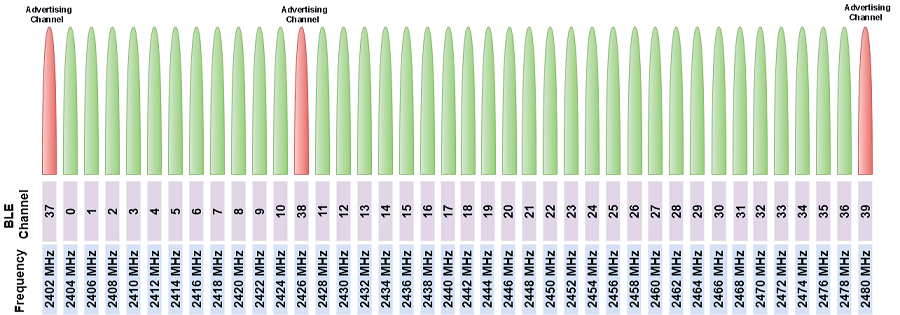
\includegraphics[width = .8\textwidth]{images/xxBLEChannels.png}
    \caption{Frequency Band Bluetooth Low Energy}
    \label{fig:freq_band_ble}
\end{figure}


\newpage
\section{Connection via Bluetooth Low Energy (BLE)}
Electric scooters use Bluetooth Low Energy (BLE) to communicate with the user's cell phone. E-scooter accomplishes this communication through Nordic Semiconductor's nRF51822 chip, which is an ultra-low power 2.4 GHz wireless system on chip 16. In figure \ref{fig:app_screen} we can see the official iOS App for the Ninebot electric scooter that can be used to retrieve information about it and manage its settings:

\begin{figure}[!htp]
    \centering
    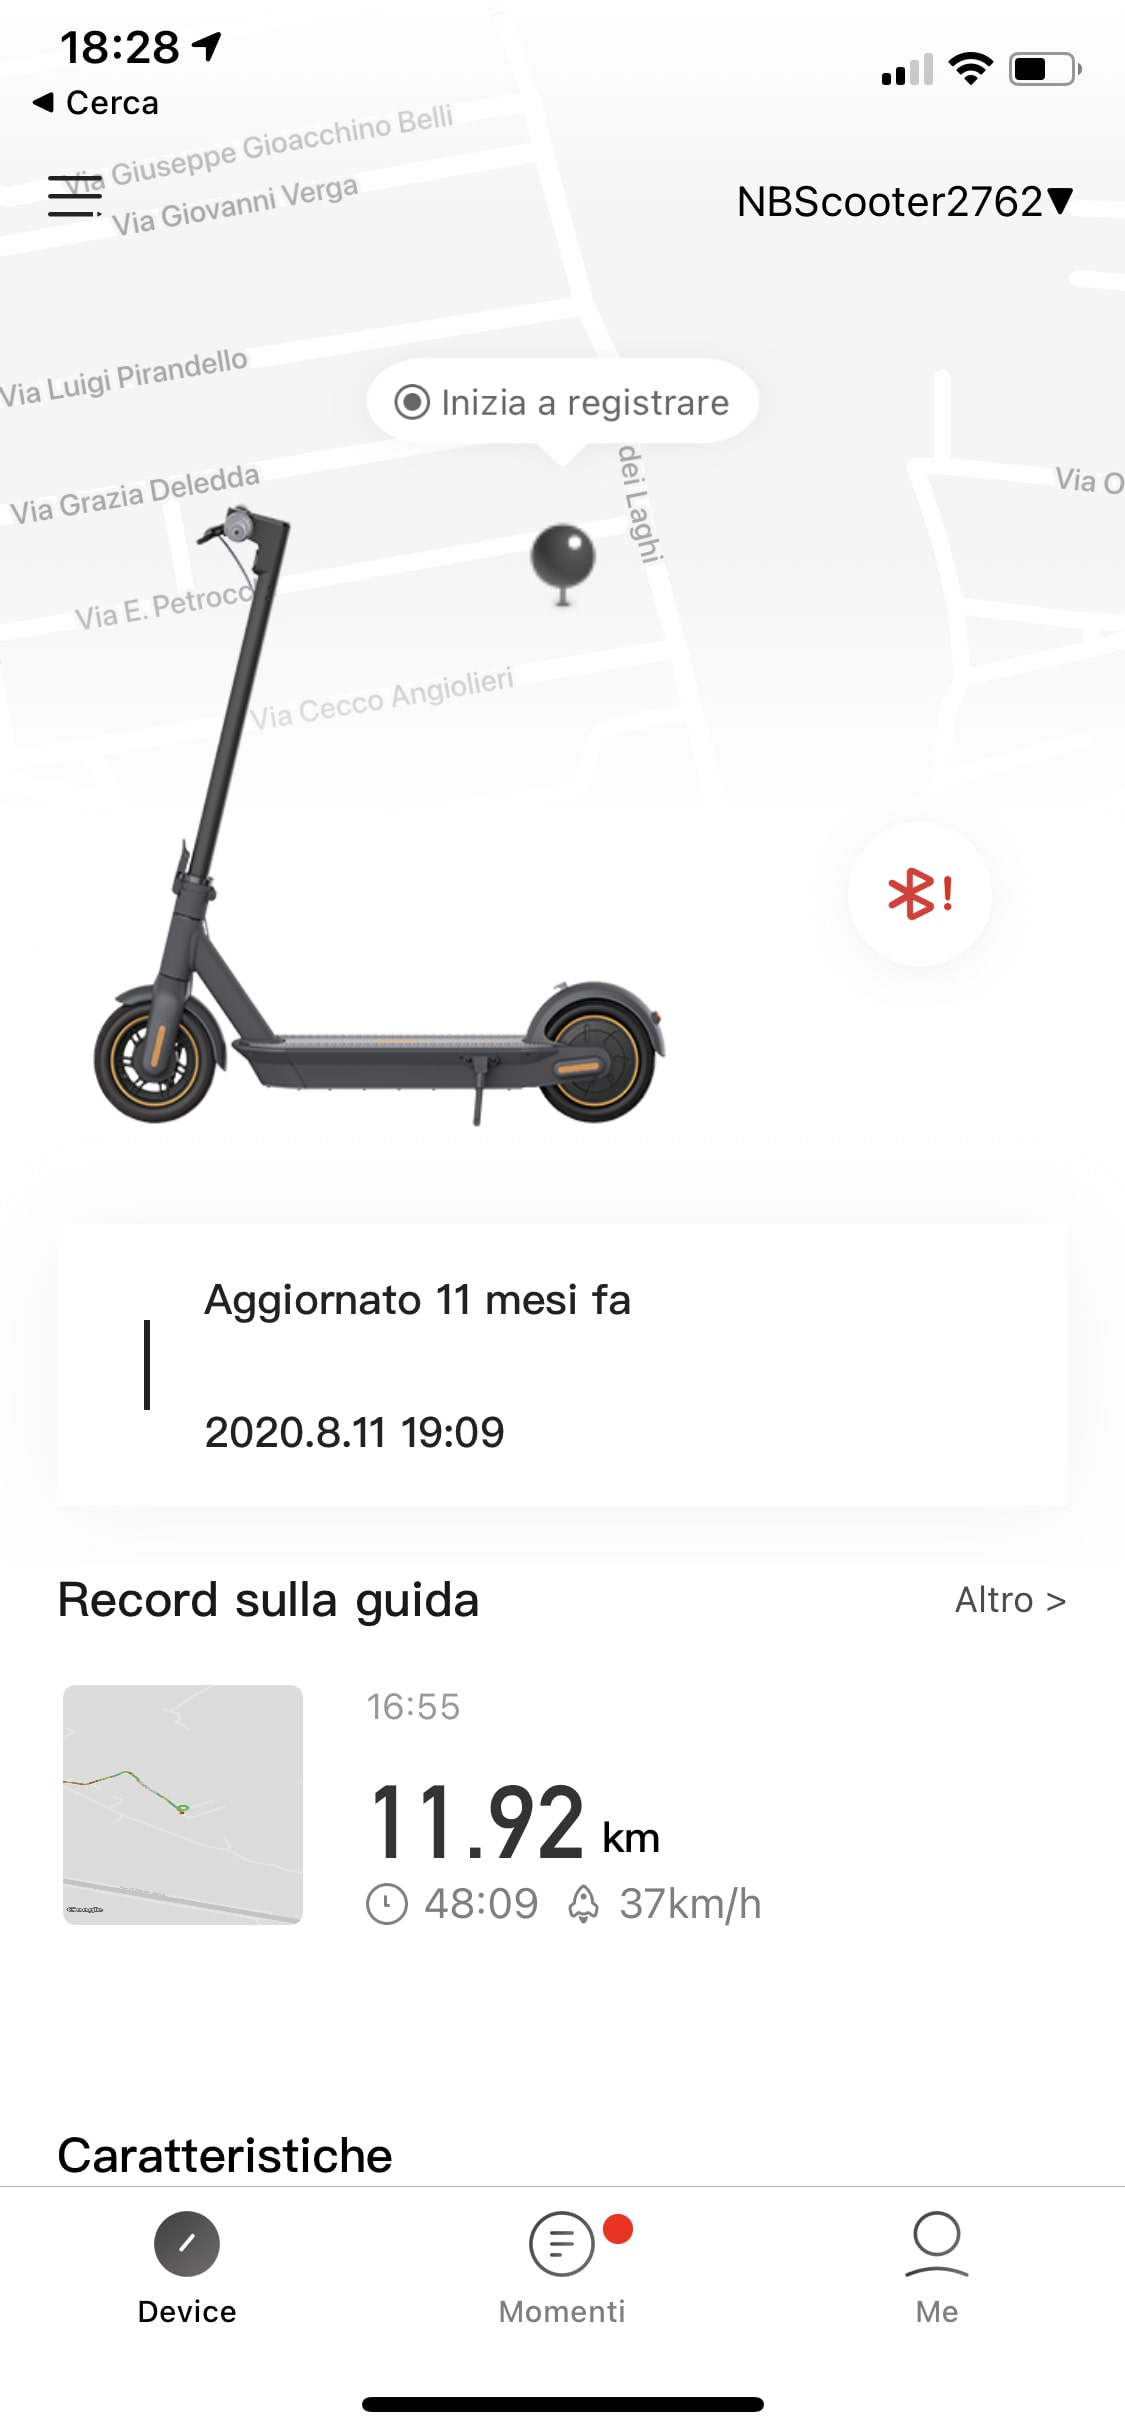
\includegraphics[width = .3\textwidth]{images/ninebot_app.jpeg}
    \caption{Ninebot iOS Application}
    \label{fig:app_screen}
\end{figure}

\noindent The electric scooter comes with pre-installed firmware, which can be updated from the manufacturer's app via Bluetooth Low Energy. The firmware runs on the e-scooter's 32-bit Cortex-M3 processor core and is compiled on the ARM-7 17 architecture. It defines many aspects related to the functionality of the electric scooter, including the internal speed limit, defines the power supplied by the battery to the motor, the speed of acceleration and more.\\

\noindent The exchange of data over Bluetooth Low Energy occurs after the pairing process between the connected devices and usually takes less time than a traditional Bluetooth connection. Both the authentication at the moment of the connection request and the encryption of the exchanged data are decided by the developers of the system used. This feature is suitable for situations where it is necessary to support a long-term connection with little data exchange between two devices.
Several tools can be used to be able to perform the BLE connection, such as \textit{hcitool}, \textit{gatttool} or \textit{BetterCAP}. Once \textit{BetterCAP} is launched, we can proceed with a Bluetooth Low Energy scan using the \lstinline[basicstyle=\ttfamily, language=bash]|ble.recon| command, which will search for BLE devices and access their advertising services. We can then stop scanning once our device is found and save its address. In figure \ref{fig:bettercpa_scan} we can see the results of the scan command with \textit{BetterCAP} tool.

\begin{figure}[!htp]
    \centering
    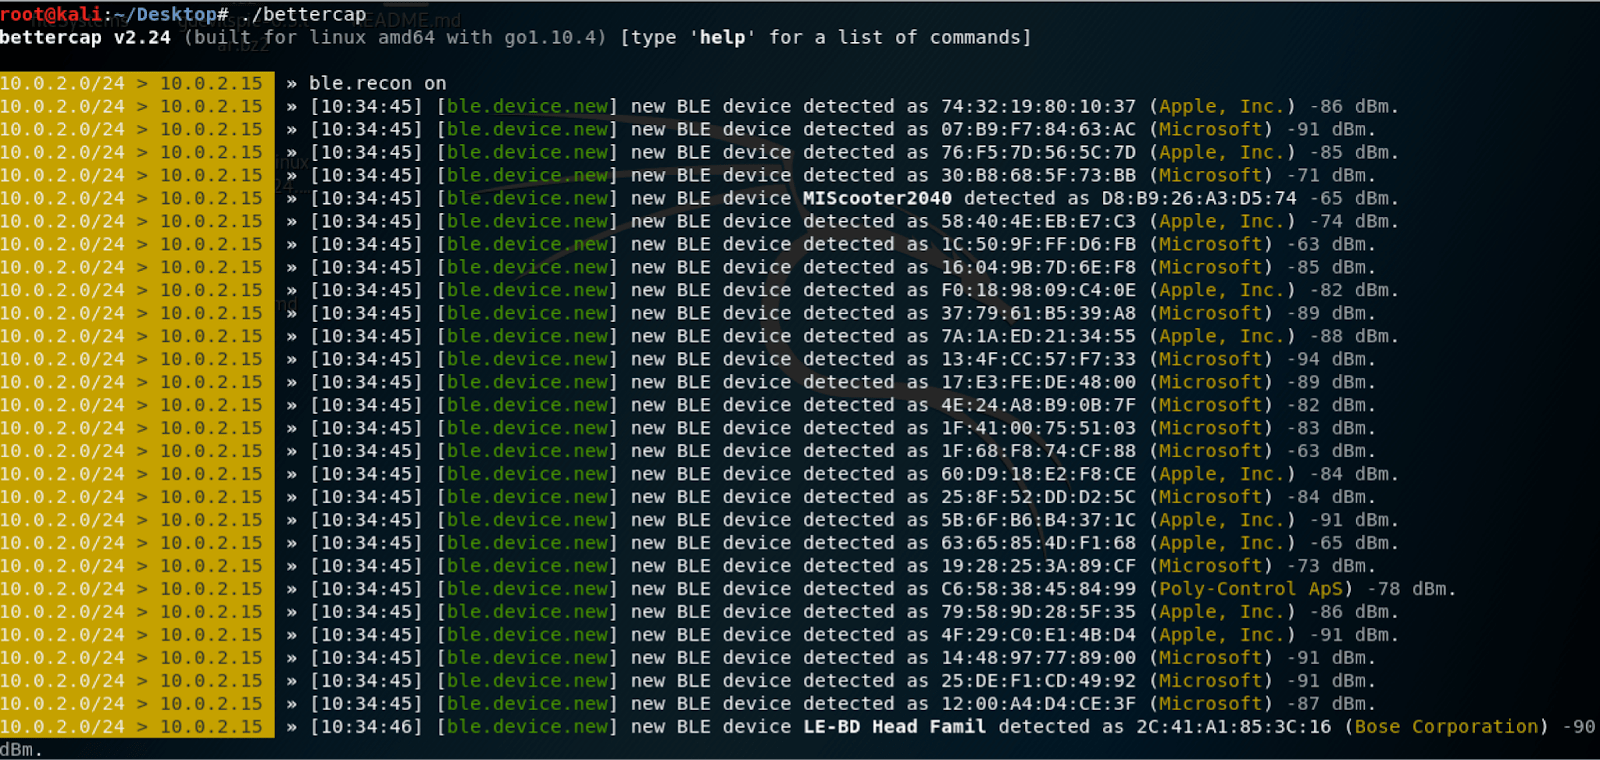
\includegraphics[width = .9\textwidth]{images/p22_7.png}
    \caption{Bluetooth scan via Bettercap}
    \label{fig:bettercpa_scan}
\end{figure}


\noindent At this point we can perform a multitude of actions on the device associated with this address. Bettercap will attempt to connect to the electric scooter first, perform the action, and disconnect immediately. We can enumerate its information using the \lstinline[basicstyle=\ttfamily, language=bash]|ble.enum|. Through the command \lstinline[basicstyle=\ttfamily, language=bash]|ble.enum MAC ADDRESS| we can also update the characteristics of the BLE firmware, values that we don't know yet and that can be found in several ways: by reverse engineering the e-scooter firmware of the mobile application or by sniffing the traffic between the electric scooter and the application. Usually the values that describe the characteristics of the device and that are written on Bluetooth Low Energy are encrypted and authenticated, however the firmware sniffed by the application and the data obtained from the server requests didn't have any kind of encryption.\\

\noindent In 2019, a cybersecurity company named Zimperium publicly released a code snippet that allows you to lock and unlock any m365 scooter. They released their exploit in the form of an iOS and Android app that allows an electric scooter to be unlocked or locked regardless of the password set by the owner, and they use the phone's Bluetooth capabilities to interact with the e-scooters to perform nefarious actions. According to Zimperium, \textit{"During our research, we determined that the password is not properly used as part of the authentication process with the electric scooter and that all commands can be executed without the password. The password is only validated on the application side, but the scooter itself does not track the authentication status."}\\

\noindent Through the use of Bettercap, we found values for the scooter's Bluetooth capabilities by performing a man-in-the-middle attack using one of the best BLE hacking software, gattacker. This allowed us to monitor traffic between a smartphone running the Ninebot or Xiaomi app and the electric scooter. We activated the lock and unlock commands on the app and took note of the data sent from the phone to discover the values used to initiate these actions in the scooter. This procedure was simply performed in an attempt to learn more about the Bluetooth Low Energy process and to obtain firmware values that would later be modified to finalize this project. Using the read command in Bettercap we were able to get more information regarding the Bluetooth Low Energy firmware of the e-scooter we are analyzing. This is shown in figure \ref{fig:m365_ble_stack}:

\begin{figure}[!htp]
\tikzstyle{freecell}=[fill=black!10,draw=black!30!black]
\tikzstyle{occupiedcell}=[fill=blue!10!orange!10,draw=blue!30!black]
\tikzstyle{padding}=[fill=yellow!20,draw=blue!30!black]
\tikzstyle{highlight}=[draw=orange!50!black,text=orange!50!black]
    \centering
\begin{drawstack}
\tikzstyle{freecell}=[fill=green!10,draw=green!30!black]
  \cell{boot}[fill=green!10,draw=green!30!black] \cellcomL{16 KB}
  \tikzstyle{freecell}=[fill=blue!10,draw=blue!30!black]
  \cell{User Data} \cellcomL{3 KB}  \cellcom{0x0003C000} 
  \padding{2}{Firmware Buffer} \cellcomL{71 KB} \cellcom{0x0003B400}  % \cellround{Yes, this one!}
  \tikzstyle{padding}=[fill=orange!20,draw=orange!30!black]
  \padding{2}{Firmware} \cellcom{0x00018000}  \cellcomL{70 KB} \cellcom{0x00029800}
  \tikzstyle{freecell}=[fill=violet!10,draw=violet!30!black]
  \cell{S110} \cellcom{0x00000000} \cellcomL{96 KB} 
  \tikzstyle{freecell}=[fill=black!10,draw=black!30!black]
\end{drawstack}

\caption{Xiaomi M365 Bluetooth Low Energy Stack}
    \label{fig:m365_ble_stack}
\end{figure}



\newpage
\section{Serial Connection}
Serial connection is a much more complex and articulated procedure compared to flashing the firmware by phone, since the latter uses only a device with Bluetooth connection. In order to connect the electric scooter to the PC via serial connection, it will be necessary to disassemble it, remove the BMS controller and once the soldering has been done on it, it will be possible to connect a ST-LINK cable to the computer and flash the firmware.\\
As shown in figure \ref{fig:conn_pins}, you must solder 3 dupont cables to the positive, negative and ground of the PCB and use the STM Utility programmer of ST-LINK that will allow you to connect to the ESC and import the binary firmware to write directly on the board.

\begin{figure}[!htp]
    \centering
    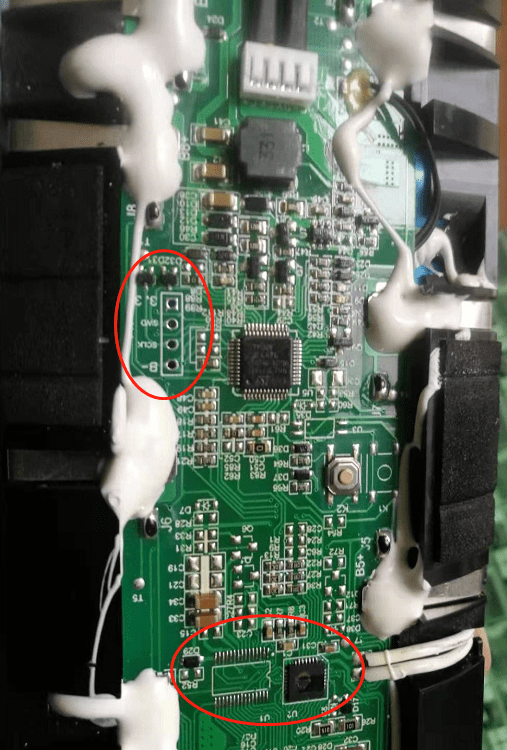
\includegraphics[width = .5\textwidth]{images/unknown-2.png}
    \caption{Ninebot Max G30 PCB connection pins}
    \label{fig:conn_pins}
\end{figure}

\noindent This section will not be discussed in detail because the custom firmware generated for this project will be flashed through a simple iOS or Android application and therefore this mode of access to the firmware of the electric scooter, although available, will not be used for the purposes of this project. It was mentioned for the sole purpose of showing the multiplicity of ways in which you can access the firmware of the e-scooter but unless specific reasons is always preferable to use the most convenient and less invasive mode.


\chapter{Electric scooter internal}
The newly purchased electric scooter comes with a pre-installed firmware that can be updated from the manufacturer's official application via BLE. This firmware, running on the e-scooter's 32-bit Cortex-M3 processor core and compiled into the ARM-7 architecture, defines many aspects of the vehicle's functionality, allowing you to set the statutory speed limits you intend to use, making changes on acceleration (e.g. quadratic or linear) or on the power supplied by the battery to the engine and many other important parameters.

\section{DRV, BMS, BLE}
To understand how the scooter firmware works, it was necessary to sniff the packets transmitted by its official application as soon as the smartphone and the electric scooter start communicating via Bluetooth. This is useful for understanding the type of information exchanged between the two parties and what is contained within the firmware binary file. From this operation we were able to understand that the e-scooter uses 3 different firmwares, each of them used to allow communication between the various mechanical parts. 
\begin{itemize}
    \item \textbf{BLE}: is the acronym for Bluetooth Low Energy, that is the wireless connection system that our electric scooter has. In the vast majority of e-scooters the Bluetooth Low Energy board is located on the handlebars. This type of firmware is responsible for "talking" with the ESC (i.e., Electronic Speed Controller) and also reads all the data from the brake lever and accelerator. It is also responsible for managing the 3 driving modes that most electric vehicles have (eco, drive and sport), as well as controlling the power button and the light.
    
    \newpage
    \begin{figure}[!htp]
    \centering
    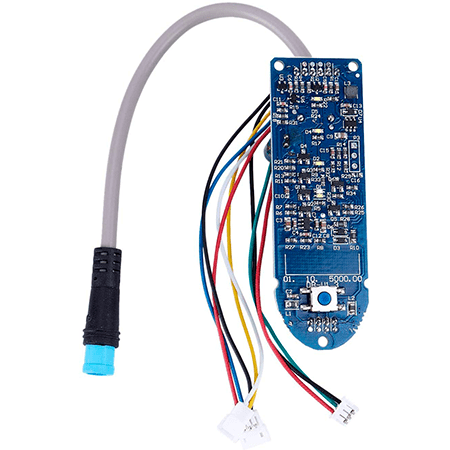
\includegraphics[width = .5\textwidth]{images/dashboard.png}
    \caption{Xiaomi M365 BLE hardware components}
    \label{fig:my_label}
    \end{figure}

    \item \textbf{ESC} (or DRV): it is the abbreviation for Electronic Speed Controller. It is the controller that handles everything related to speed control to the motor. It is important because to control a brushless DC motor it is necessary to use a particular firmware that manages the electronic controller.
    
    \item \textbf{BMS}: stands for Battery Management System. The BMS is a board that manages the batteries and their cells, thanks to this controller we can have all the cells well balanced and know the status of each of them by managing the power delivered by the motor with respect to the available charge and also manipulating the charging phases. and battery discharge.
\end{itemize}

\noindent To find out the version number of each of the 3 firmwares just use the manufacturer's native application or one of the third-party applications available on AppStore and PlayStore, like M365Tools.

\section{DRV Parameters}
The firmware that we are interested in modifying is the DRV, in fact we want to bring some precautions to increase the safety of the guided electric scooter in combination with a wheelchair for the disabled and possibly also modulate the performance of the e-scooter trying to reach a good compromise between the power delivered and battery charge. As mentioned above the firmware allows to manipulate a very high number of parameters. Below we will show some parameters of interest that were used during the project:
\begin{itemize}
    \item \underline{Wheel speed multiplier}: Allows to show on the display the correct speed according to the type of tires mounted on the electric scooter. For example Xiaomi M365 mounts 8.5 inch wheels by default, in this case the value is 345. We focus on this parameter because in order to ensure greater driving comfort to a disabled person, it was decided to mount tubeless tires with a larger diameter of 10 inches and therefore not a full tires. In this case the wheel speed multiplier is 315. 
    \item \underline{Cruise control}: The automatic speed control option has been "borrowed" from cars. Most scooters (but also electric scooters) make use of a similar algorithm to cars for constant speed. Cruise control leverages data received from 3 sensors regarding: engine Rotation-Per-Minute, battery voltage and power used. The electric scooter's control unit uses the signals received from the sensors as input and is able to control the power of the motor. If the sensors detect that the required speed is constant, they keep the motor power constant (i.e., flat road), while if they detect that the speed is decreasing, they increase the motor power until the required speed is reached and kept constant (i.e., uphill road). \\ 
    It represents a great advantage especially on long journeys, especially on a straight road, because it can make driving more comfortable and avoid hand fatigue, avoiding having to press the acceleration knob continuously. This function is very convenient if the driver is a normal person, but it could represent a danger in case of a disabled person, as maintaining the speed even when going downhill does not guarantee the user a safe driving. This aspect must be taken into consideration and therefore modulated to avoid causing damage to the person using the electric scooter.
    
    \item \underline{KERS}: Kinetic Energy Recovery System is an electromechanical device that transforms kinetic energy into mechanical or electrical energy during braking, allowing a partial recovery of energy. This system is generally made up of a motor/dynamo, an energy accumulator (electrical or mechanical) and a control system.
    
    \begin{figure}[!htp]
    \centering
    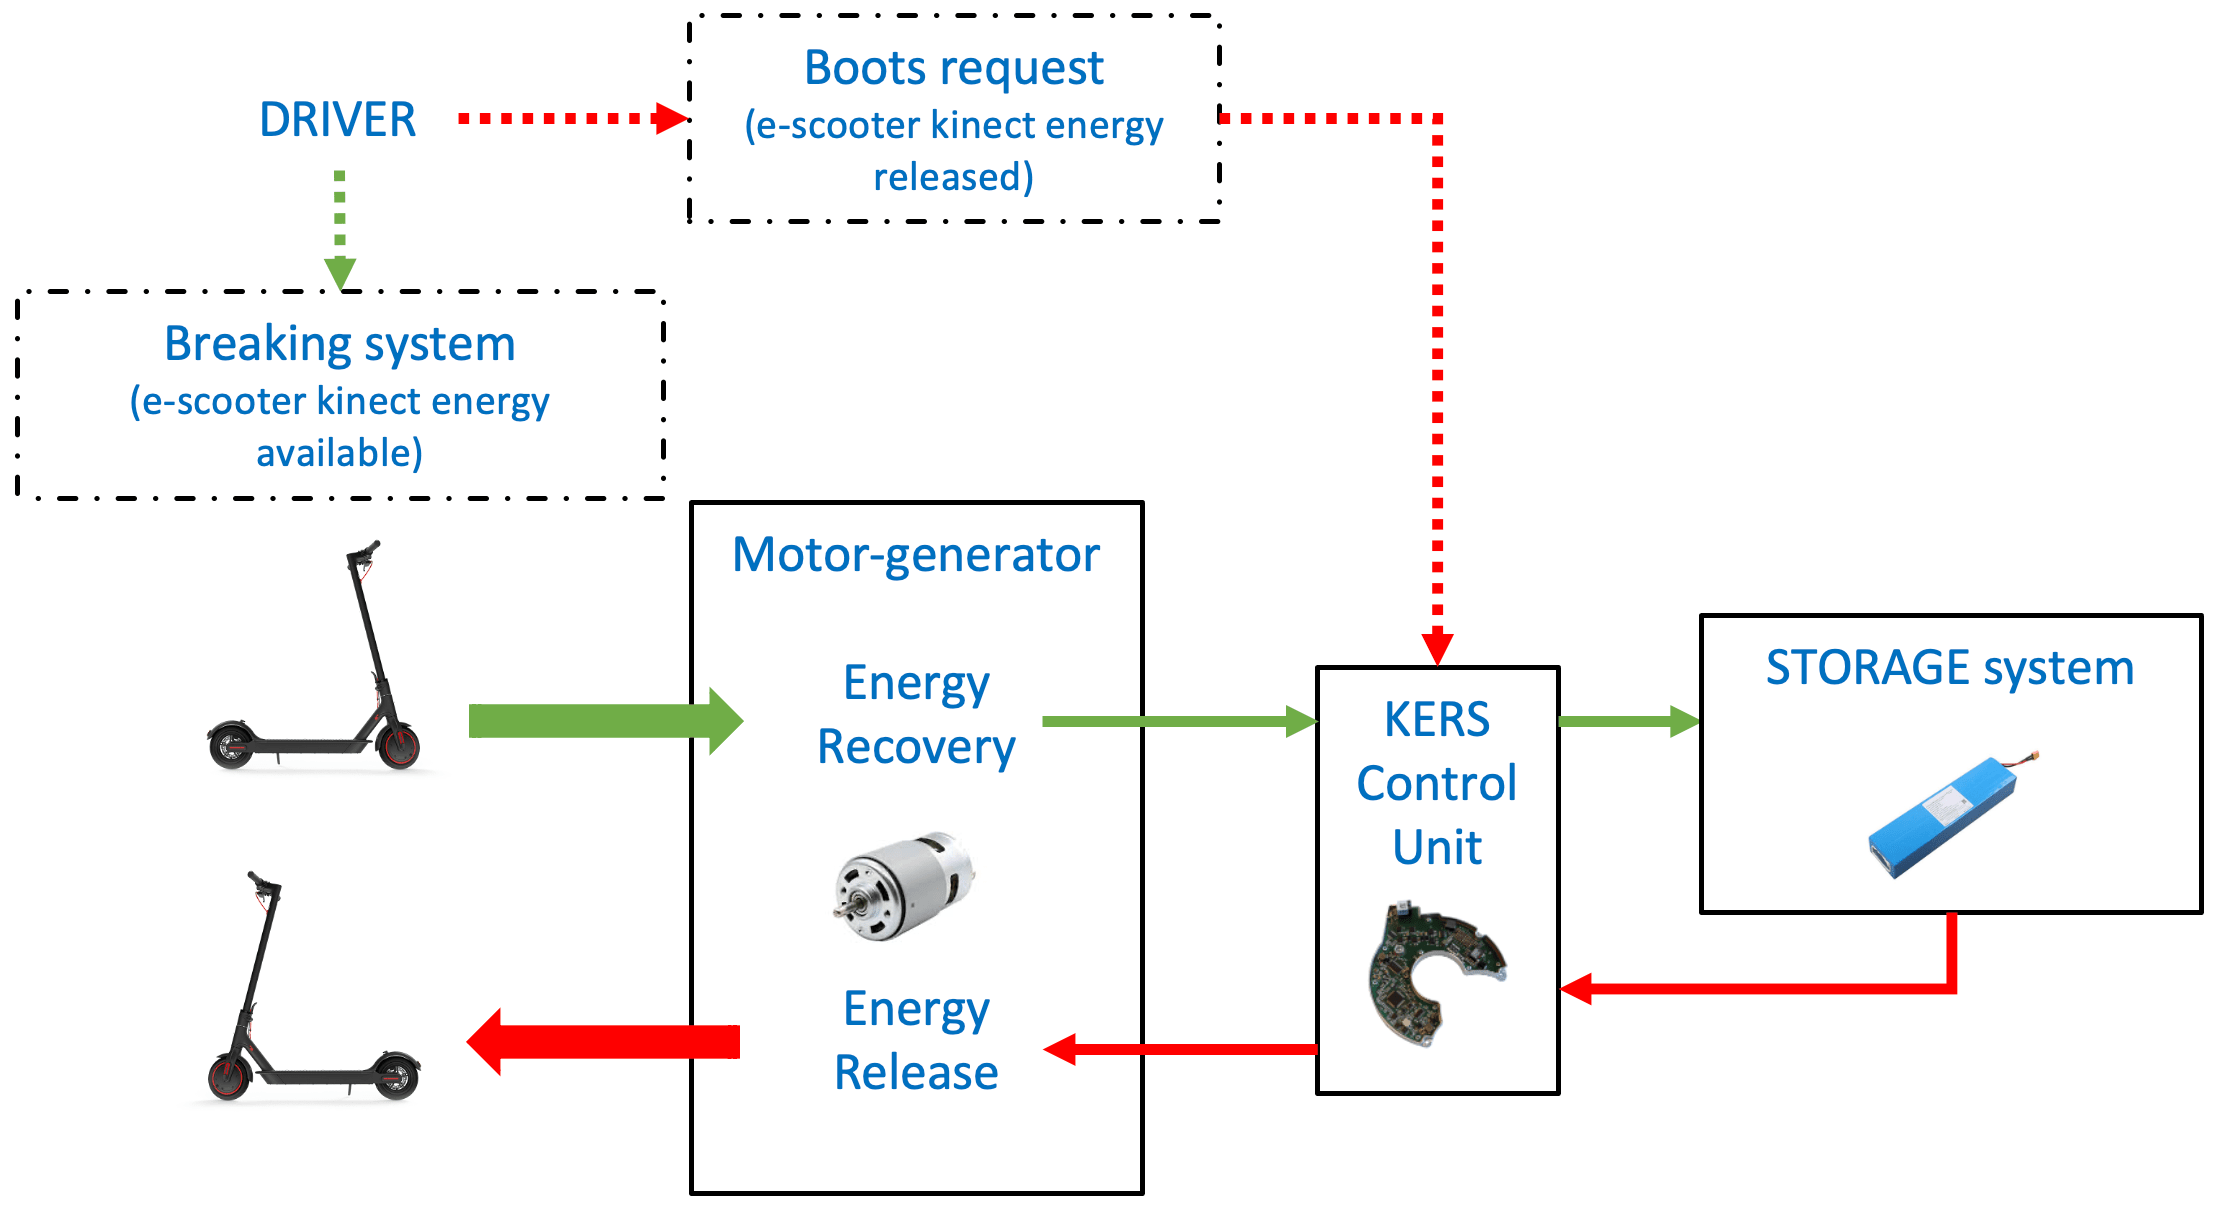
\includegraphics[width = .9\textwidth]{images/kers.png}
    \caption{KERS functioning}
    \label{fig:my_label}
    \end{figure}
    
    \noindent In the  apps that allow the management of electric scooters with stock firmware via Bluetooth, the energy recovery is often customizable on 2 or 3 levels, namely low, medium and high. It acts in two phases, when you release the accelerator and when you brake. The first one recovers energy when you release the accelerator, the second one integrates the braking of the main brake with the one produced by the engine brake (for example on Ninebot it brakes electronically at the rear when you activate the drum brake at the front). With the stock firmware the first is deactivable and the second is not.\\ 
    KERS is an element that not only recovers energy during braking and deceleration but also protects the circuits from the so-called "over voltage" even if many users keep it deactivated without problems. \\
    The KERS is inversely proportional to the "motor power constant" and bound to it. In fact, at low engine power constants, braking will be abrupt and the same applies to when you leave the accelerator; setting a high value for the engine power constant instead, braking will be less abrupt and therefore softer.\\
    \noindent However, the KERS has a downside, that is, on the stock firmware it constantly acts, both in braking and in deceleration and it is not possible to disable it as most electric scooters are not equipped with both braking modes: electric brake and drum brake. Precisely for this reason it was decided to make a hardware change to the e-scooter by mounting an electric brake as an “accessory” that acts as a lever to manually operate the KERS. This change was made because the sum of the weight obtained by the wheelchair and the electric scooter is considerable and braking with the drum brake alone would increase the braking distance, thus decreasing driving safety.
    
    \begin{figure}[!htp]
    \centering
    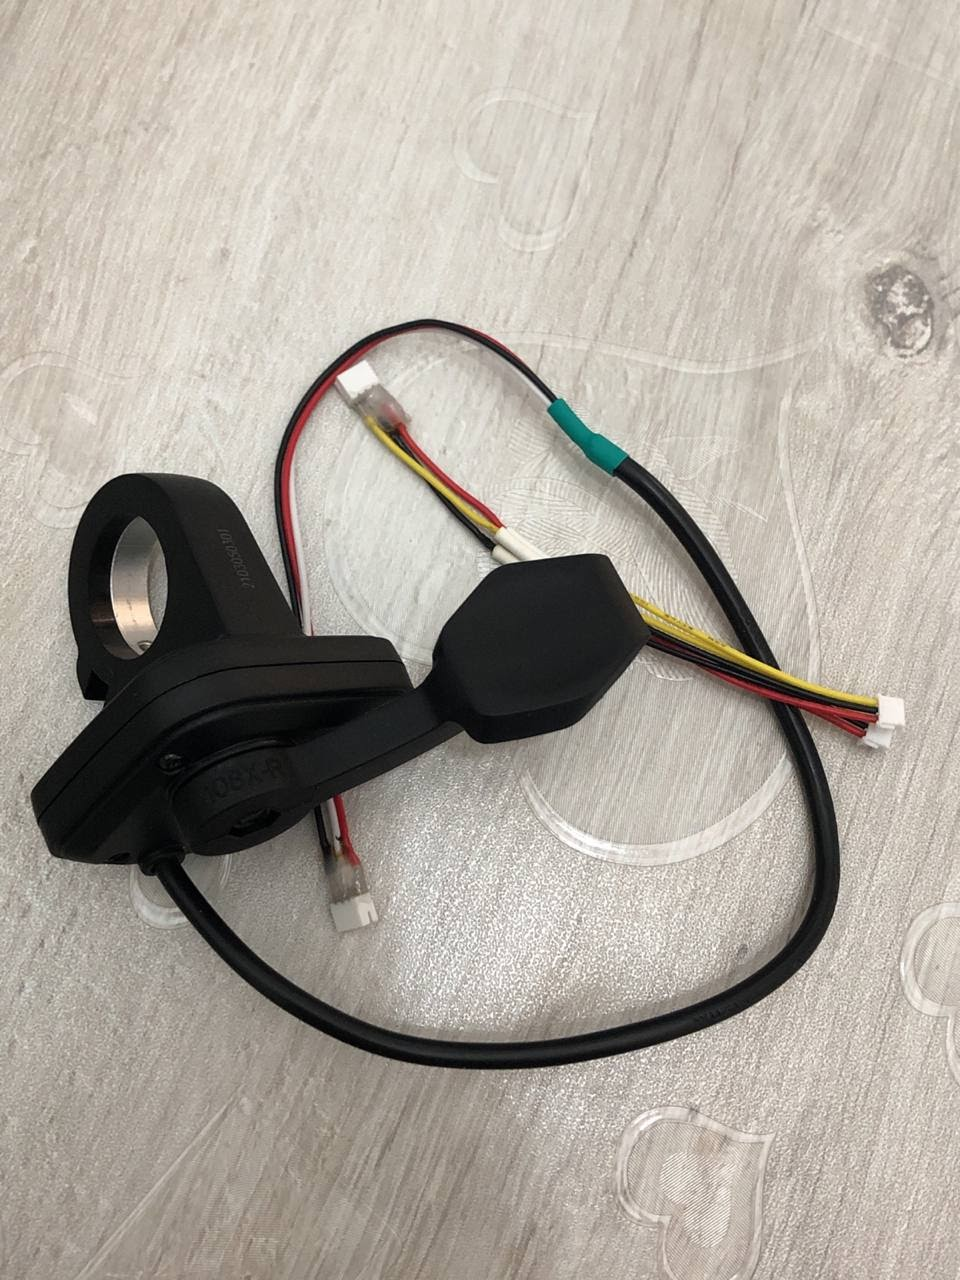
\includegraphics[width = .5\textwidth]{images/leva_freno.jpeg}
    \caption{Additional brake lever}
    \label{fig:my_label}
    \end{figure}
    
    \noindent In this way it is possible firmware side to disable the automatic KERS and enable it in manual mode to prevent abrupt driver braking.
    
    \newpage
    \begin{figure}[!htp]
    \centering
    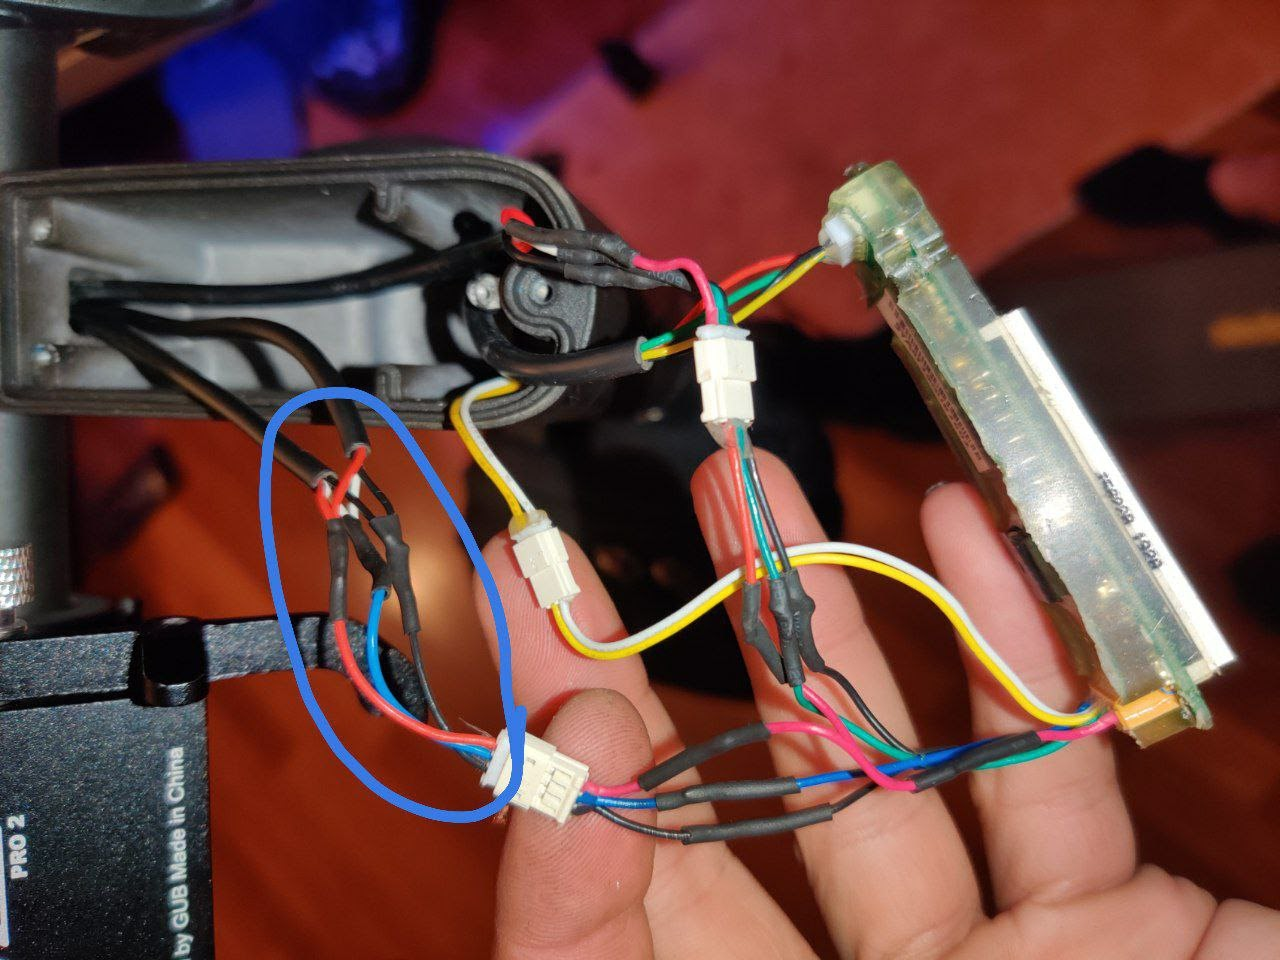
\includegraphics[width = .7\textwidth]{images/collegamenti_leva.jpeg}
    \caption{Brake lever connections}
    \label{fig:my_label}
    \end{figure}
    
    \item \underline{Motor Power Constant}: Motor Power Constant and KERS parameters are two elements related to each other and necessary when it comes to use custom firmware to modify the power or speed of electric scooters. Speaking in purely theoretical terms, Motor Power Constant represents the ability of the motor to convert the power of electricity into mechanical power. The motor constant is given by:
    \begin{equation}
        k_m = \frac{T}{\sqrt{P}}
    \end{equation}
    where: \begin{itemize}
        \item $K_m$ = constant of the motor $(Nm/\sqrt{Watt}) $
        \item $T$ = torque ( $Nm$ )
        \item $P$ = resistive power losses (also known as $I^2 \times R$ losses ) ($W$)    
    \end{itemize}
    The Motor Power Constant is a value that increases the power output inversely proportional to the number set, i.e., the lower the number, the higher the power.\\
    This parameter will have to be decreased to guarantee a greater thrust to the electric scooter when towing the wheelchair.\\
    Increasing this value will reduce the acceleration and power of the engine, obtaining much more autonomy, while decreasing it you will get an increase in thrust and power, but paying for autonomy. This parameter can assume values in a range between 25000 and 50000.\\
    After various performance and stability tests it was decided to apply a lower limit of 45000, a value below which it is necessary not to go down.
\end{itemize}

\noindent In the following we will analyze further parameters and the optimal values identified for them:
\begin{itemize}
    \item \underline{Motor Start Speed}: Electric scooters need a minimum push to start moving. Through this parameter it is possible to decrease the activation speed of the vehicle. By default this value is set to 5 km/h. This starting speed has been deactivated to allow starting from standstill and to allow towing the wheelchair. 
    \item \underline{Current Raising}: this value determines the speed with which the control unit passes from one current level to another (acceleration). For the standard 36v battery, a value of this parameter between 1200-1500 mA/step is recommended for rapid acceleration. If in the future you decide to upgrade the battery to 48V, this value can be set to 2500-3000 mA/step for an even more aggressive acceleration.
    \item\underline{DPC Curve}: this is one of the most important parameters to modify when the electric scooter is driven by a person in a wheelchair. Stock e-scooters use an acceleration algorithm called "Speed Based Throttle" that makes each position on our throttle correspond to an expected speed. For example a 20\% rotation of the accelerator will bring the scooter to 20\% of its maximum speed, 50\% to 50\% until you reach 100\% where the scooter will take you to the maximum possible speed. In practice the electric scooter will force the motor to run at high power until it reaches its intended speed (e.g., 20 km/h), then stop, and then again at the power needed to maintain a constant speed. This process is perceived by the driver as jerky movements, which results in a not perfectly smooth ride. Full power will be delivered only when necessary, e.g., a standing start or a climb.\\
    With the speed-based algorithm, the acceleration curve is linear and proportional, as shown in figure \ref{fig:linear_curve}.
    
    \begin{figure}[!htp]
    \centering
    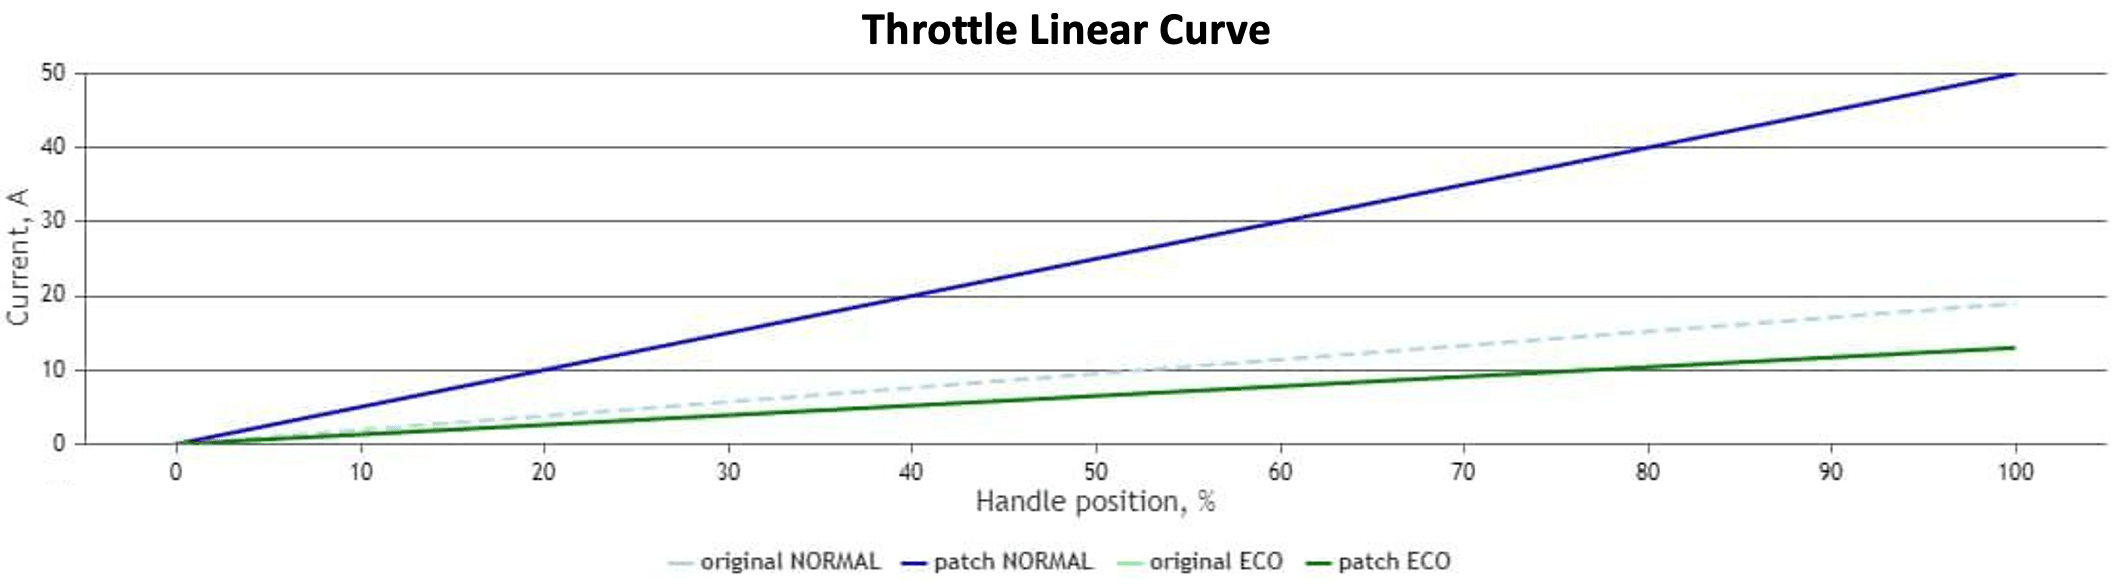
\includegraphics[width = .9\textwidth]{images/linear.png}
    \caption{Throttle Linear Curve}
    \label{fig:linear_curve}
    \end{figure}
    \noindent "Current Based Throttle Algorithms" is a type of algorithm according to which a given rotation of the accelerator corresponds to a total power output in terms of Watts and not to a speed as in the standard firmware of the electric scooter.  For example, a half-turned throttle will correspond to a delivery of half the total power of the e-scooter in terms of Watts and keeps it constant. This allows for a much smoother ride because it represents the same principle as any heat engine we have ever dealt with. For example the car, to a total amount of pressure administered to the pedal corresponds an amount of power delivered and not a predefined speed. With 100\% throttle with a current based protocol the electric scooter will give the motor maximum power up to the maximum rotation speed then limited by the battery voltage.\\
    With the current-based algorithm, the output power works in logarithmic scale, so the power will be sweet in the low end and then go up on the final. The acceleration curve is shown in the figure \ref{fig:quad_curve}.
    
    \begin{figure}[!htp]
    \centering
    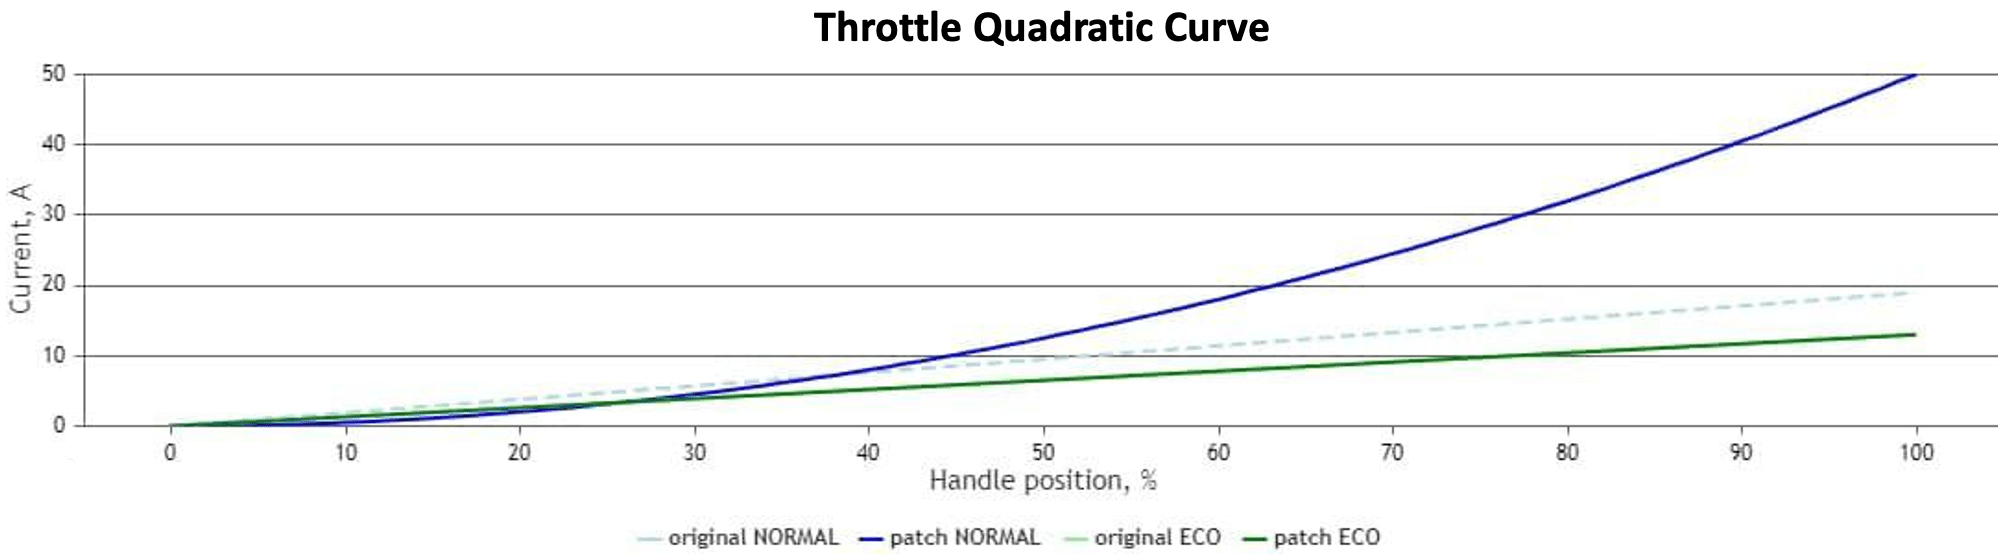
\includegraphics[width = .9\textwidth]{images/quadratic.png}
    \caption{Throttle Quadratic Curve}
    \label{fig:quad_curve}
    \end{figure}
    
    \item \underline{Max Speed}:  The title is already quite clear, this item allows you to set the maximum speed in a given mode (Eco, Drive and Sport). This value will have to be decreased to limit the maximum speed of the electric scooter driven by a disabled person.
    
    \item\underline{Version Spoofing}: This parameter allows you to trick the official app into believing it has an already updated version, so the user will be able to use the original app that won't offer the official update that would inevitably make the user lose the changes made.

\end{itemize}

\section{Electric Scooter Communication Protocol}
\noindent Before analyzing the components that allow you to interface the electric scooter with devices such as computers or smartphones, it is necessary to know the communication protocols used by the main manufacturers of electric scooters, namely Ninebot and Xiaomi.

% Define block styles
\tikzstyle{decision} = [diamond, draw, fill=blue!20,
    text width=4.5em, text badly centered, node distance=2.5cm, inner sep=0pt]
\tikzstyle{block} = [rectangle, draw, fill=blue!20,
    text width=7em, text centered, rounded corners, minimum height=4em]
\tikzstyle{line} = [draw, very thick, color=black!50, -latex']
\tikzstyle{cloud} = [draw, ellipse,fill=red!20, node distance=4cm,
    minimum height=2em]
    


\begin{figure}[!htp]
    \centering
    \begin{tikzpicture}[thick,scale=0.7, every node/.style={scale=0.7},node distance = 2.6cm, auto]
        % Place nodes
        \node [block] (init) {Bluetooth LE};
        \node [cloud, left of=init] (Phone) {Phone};
        \node [block, below of=init] (3) {Single wire half-duplex UART 115200 8n1};
        \node [block, below of=3] (4) {ESC};
        \node [block, below left of=4] (51) {Two wire UART 115200 8n1};
        \node [block, below right of=4] (52) {BMS};
        
        \path [line,dashed] (Phone) -- (init);
        \path [line] (init) -> (3);
        \path [line] (3) -> (4);
        \path [line] (4) -> (51);
        \path [line] (4) -> (52);
    \end{tikzpicture}
    \caption{Xiaomi/Ninebot Protocol}
    \label{fig:protocol_1}
\end{figure}

\noindent 
The protocol illustrated in the figure \ref{fig:protocol_1} defines the general format with which the Ninebot and Xiaomi electronic control system realizes the multi-node communication through physical serial ports and Bluetooth serial ports. To use the serial port communication it is necessary to use a baud rate of 115200, 8 byte words, without verification and with 1 stop bit. Information retrieval, control and parameter modification can be accomplished through a read-write operation on the "memory control table" which is stored in the controller. The basic storage unit of the memory control table is 2 bytes of signed (short) integer data.\\
All data longer than 1 byte is subject to the low-priority transmission and storage form.\\
Xiaomi and Ninebot use the same communication protocol but they exchange packets of different values and size. More precisely, in the instruction packet that reads and writes the memory control table and in the read response packet, data index indicates the offset address of the data accessed in the table; in the response packet (command word 0x05) with the response write operation, the data index 0 indicates a successful write. Other values are defined as follows:
\begin{itemize}[noitemsep, topsep=1pt]
    \item 0x01: No write permission for the write-in address.
    \item 0x02: The control table is under operation, and no write-in is allowed.
    \item 0x03: Write-in data is out of scope.
    \item 0x04: Write-in data is in wrong form.
\end{itemize}

\noindent During the firmware download, data index indicates the number of the data packet under continuous data download. When the firmware downloads related instruction response packets, data index 0 indicates download successful. Other values are defined as follows:
\begin{itemize}[noitemsep, topsep=1pt]
    \item 0x01: Firmware is over-sized
    \item 0x02: Erase Flash failed
    \item 0x03: Write Flash failed
    \item 0x04: Scooter is unlocked or firmware can be updated
    \item 0x05: Data index error
    \item 0x06: IAP is busy (such as writing in Flash)
    \item 0x07: Data format error (length of the data sent is not an integer multiple of 8)
    \item 0x08: Data verification failure
    \item 0x09: Other errors
\end{itemize}
The error values are very useful in case of firmware flashing as they immediately trace the cause of the problem and we can easily understand if the error generated is caused by a problem in the coding of our firmware or by other factors that do not derive from the firmware itself.

\subsection{Serial port reads memory control table}
If the computer wants to read current temperature of the electric scooter, as the index address of scooter temperature in the memory control table is (0x3E), instruction type shall be "read instruction", namely 0x01 and the data index is 0x3E. As the basic unit of the memory control table is a 16-bit integer data, the read length is 2 bytes. Data segment has only one byte with the value of 2 and the frame length is 1. Source ID is ID of the upper computer, 0x3D. Target ID is main control panel ID of the electric scooter, 0x20. Instruction packet sent by the upper computer is:
\begin{equation*}
    \text{5A \ A5 \ 01 \ \textcolor{red}{3D \ 20 \ 01 \ 3E \ 02} \ 60 \ FF}
\end{equation*}
Upon receiving the data packet, the electric scooter will return current body temperature value. The main control panel will return data to the upper computer according to the source ID of the packet. Therefore, the target ID is the upper computer ID, 0x3D and source ID is main control panel ID of the electric scooter, 0x20. Instruction type is 0x05 (read response) and data index is 0x3E (body temperature). Date segment is the body temperature, as it is a 16-bit data, the data segment has two bytes with the low order in front. Assume current body temperature is 31.8°C, as the temperature unit is 0.1°C, the value read is 318, namely 0x13E in the hexadecimal system. Therefore, two bytes of the data segment are 36  with the frame length of 2. The response packet returned by the electric scooter is as follows:
\begin{equation*}
    \text{5A \ A5 \ 02 \ \textcolor{red}{20 \ 3D \ 04 \ 3E \ 36\ 01 \ } 27 \ FF}
\end{equation*}
In practical application, in order to save communication bandwidth, multi-data can be read in one time, such as to read 14-byte electric scooter serial number in one time. Start address of the serial number in the memory table is 0x10, with a size of 14 byte, from 0x10 to 0x16. During reading, data index of the instruction packet is set as 0x10 and the read length (namely data segment) is set as 14, the electric scooter will return continuous 14 byte data segment, namely scooter serial number. Instruction packet sent by the upper computer is:
\begin{equation*}
    \text{5A \ A5 \ 01 \textcolor{red}{3D \ 20 \ 01 \ 10 \ 0E } 82 \ FF}    
\end{equation*}


\subsection{Serial port writes memory control table}
When data is about to be written to the memory control table, instruction type of the instruction packet shall be set as "write instruction", namely 0x02 (write instruction with response) or 0x03 (write instruction without response). 
\begin{itemize}[noitemsep, topsep=0pt]
    \item For "write instruction with response", the lower computer will return a response instruction indicating successful write after receiving the "write instruction".
    \item For "write instruction without response", the lower computer will not return such instruction, whether receiving the instruction or not.
\end{itemize}
The first type of write is used for write-in of some important data and the upper computer needs to confirm whether the lower computer receives the data or not, such as write-in of electric scooter speed limit value; the latter is used for the occasion having high requirement on real-time performance but paying less attention to the write-in, such as write-in of remote control target speed value under remote control mode.\\
For example: write electric scooter speed limit value 10 km/h under the speed limit mode with response. Index of the speed limit value is 0x74 with the unit of O.1km/h. So, the value written is 100, namely 0x0064 in the hexadecimal system. As the basic unit of the memory control table is a 16 bit integer data with the low order in front during writing, the data segment to be written is 0x64 0x00, and the whole instruction packet is:
\begin{equation*}
    \text{5A \ A5 \ 02 \ \textcolor{red}{3D \ 20 \ 03 \ 74 \ 64 \ 00 }\ C5 \ FE}
\end{equation*}
In case of successful writing, the response packet returned by the lower computer is as follows:
\begin{equation*}
    \text{5A \ A5 \ 01 \textcolor{red}{20 \ 3D \ 05 \ 74 \ 01 }\ 27 \ FF}
\end{equation*}
Like read operation, multi-data can also be written in the write operation, such as writing of Bluetooth pairing code 123456:
\begin{equation*}
    5A \ A5 \ 06 \ \textcolor{red}{3D \ 20 \ 03 \ 17 \ 01 \ 02 \ 03 \ 04 \ 05 \ 06 \ } 6D \ FF 
\end{equation*}

\chapter{Modify firmware parameters}
Electric scooters communicate with the smartphone app using established and prevalent technologies such as the Bluetooth Low Energy. However, the use of such communication channels also opens the door to too many attacks, some of which may be particularly easy and effective on electric scooters. 

\section{Sniffing Packets}
To obtain the original firmware of the electric scooter used for this project, a Man in the Middle attack was performed by "sniffing" the communication between the two entities. 
Sniffing can be defined as a process that refers to the investigation of something hidden to find confidential information. From an information security perspective, sniffing refers to intercepting traffic or routing traffic to a target where it can be captured, analyzed and monitored. It is mainly performed to analyze network usage, troubleshoot network problems, session monitoring for development and testing purposes.
Network packets or TCP/IP packets contain information required for two network interfaces to communicate with each other. It contains fields that are source and destination IP addresses, ports, sequence numbers, and protocol type. All these fields are vital for the proper functioning of the various network layers, especially for the Layer 7 application that uses the received data.\\
Thor HTTP Sniffer/Capture is one of the best network packet analyzers for iOS, it is an application that monitors traffic data to and from a computer network connection. It serves to analyze packets with the purpose of presenting captured packet data in the most detailed way possible by intercepting binary traffic by converting it into readable format, making it easy to identify what kind of traffic is going through the network, how much and how often.\\
After installing the application, clicking on the single button on the main screen sets up a DevTunnel session through which Thor will be able to capture packets crossing the network to analyze them later. Now just turn on the electric scooter and start the official application (Ninebot) to allow communication between the two entities.

\section{Analyzing sniffed packets}
Once the traffic has been monitored, it is enough to close the DevTunnel session and export the archive in .har format to carry out a careful analysis on the computer using Wireshark. 
Through this sniffing tool we were able to reconstruct a scheme that describes the type of communication that the electric scooter makes while communicating with the cloud server of the parent company. In figure \ref{fig:threat_model} we can see how the communication works among the various actor involved in it.
\begin{figure}[!htp]
    \centering
    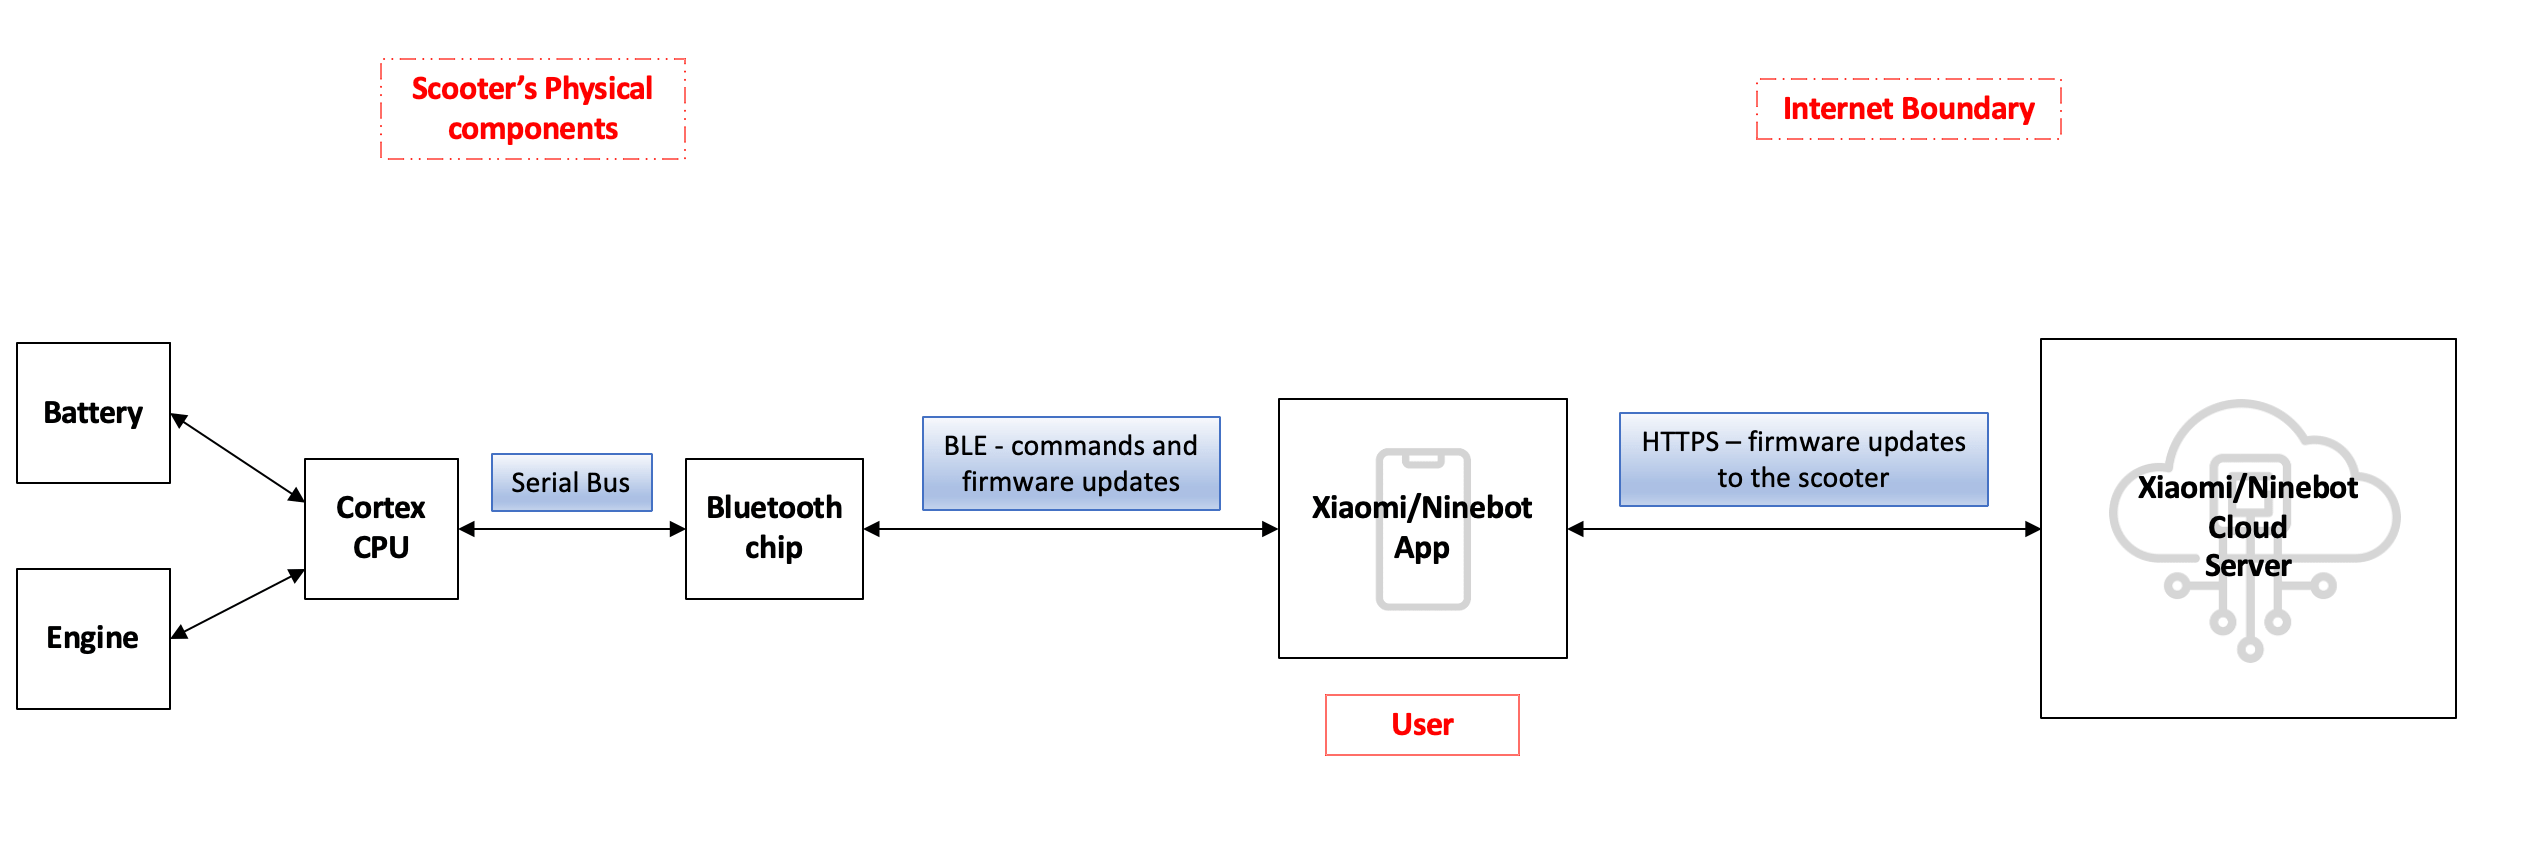
\includegraphics[width = .9\textwidth]{images/sniffing_diagram.png}
    \caption{Scooter-App Communication Diagram}
    \label{fig:threat_model}
\end{figure}

\noindent Analyzing the various HTTP requests and responses we find in clear text an endpoint that provides through simple GET/POST the firmware of the electric scooter previously connected to the application. To obtain the binary file of the firmware a Python program has been created that using three simple functions performs the same operations of the official application saving the result locally. The figures below show the result obtained from the execution of the program:
\begin{figure}[!htp]
    \centering
    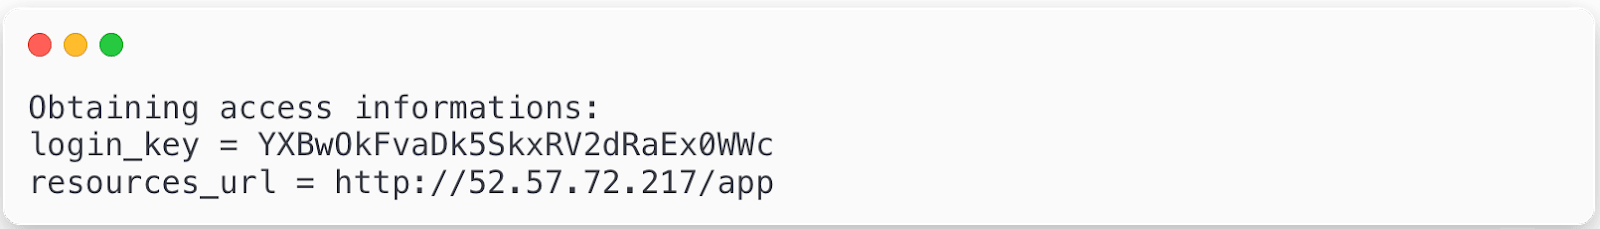
\includegraphics[width = .9\textwidth]{images/sniff1.png}
    \caption{Access Informations}
    \label{fig:my_label}
\end{figure}


\begin{figure}[!htp]
    \centering
    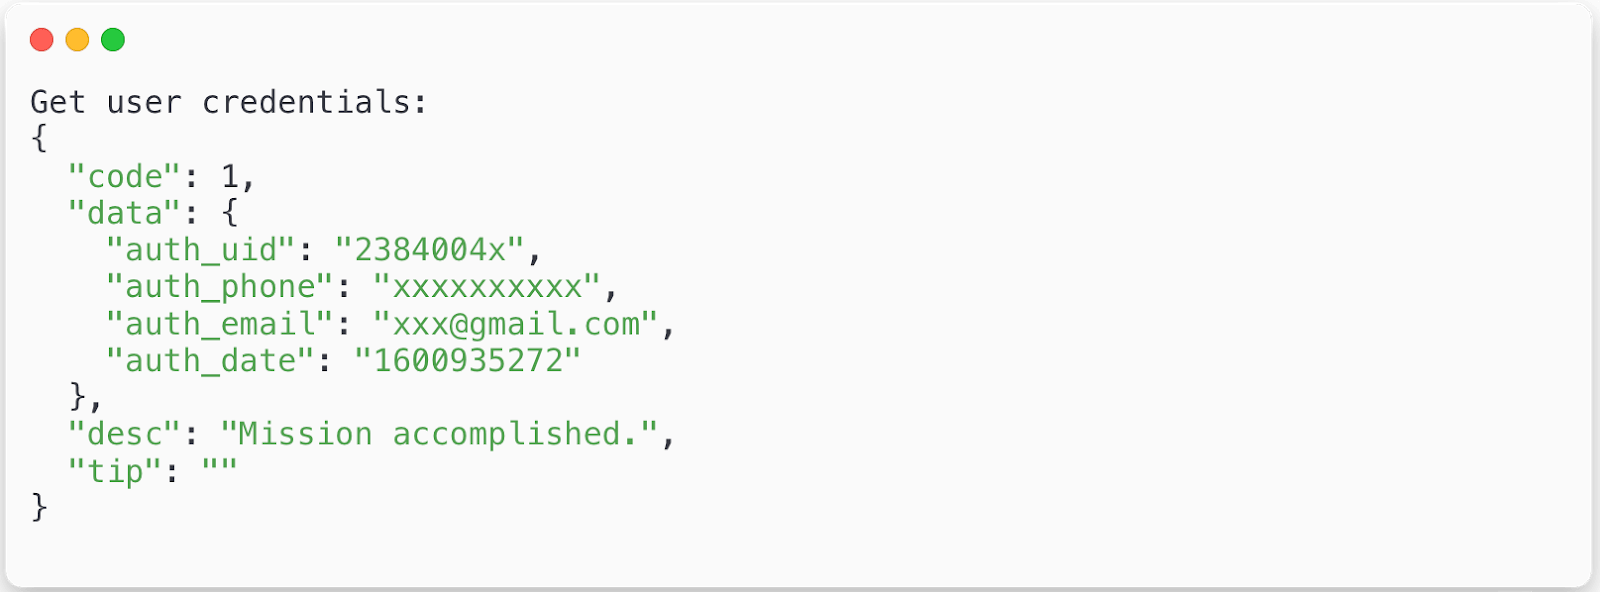
\includegraphics[width = .9\textwidth]{images/sniff2.png}
    \caption{User Informations}
    \label{fig:my_label}
\end{figure}

\begin{figure}[!htp]
    \centering
    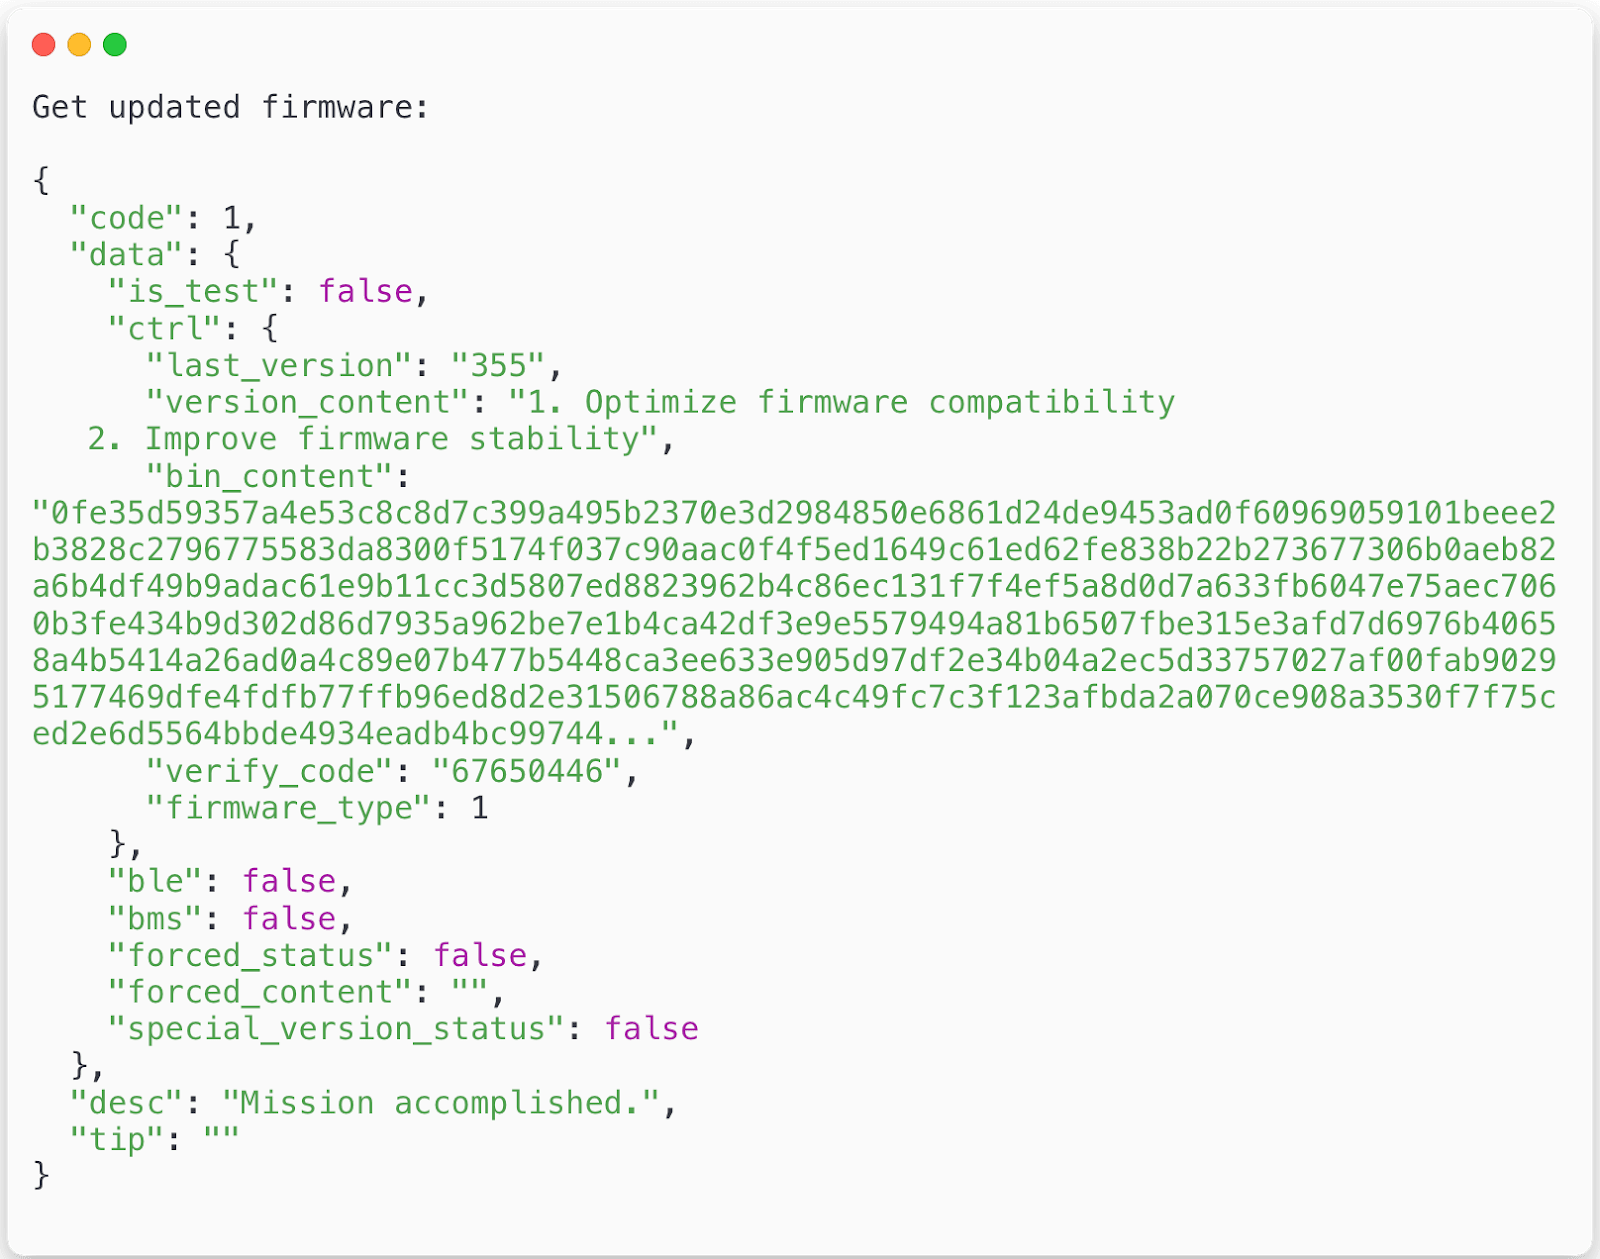
\includegraphics[width = .9\textwidth]{images/sniff3.png}
    \caption{Getting last firmware}
    \label{fig:my_label}
\end{figure}

\noindent Going to analyze the last request to the server we can see that the json key "bin\_content" returns in clear the binary file that will be used as source for the parameter modification operation.

\section{Edit stock firmware}
A first careful analysis of the binary file obtained by sniffing packets from the original application was performed with a decompiler that transforms this data structure into a readable assembly and then into a python data structure (\textit{bytearray}) that automates through various functions this process. The software used for this task is Ghidra, a tool developed by NSA that contains a set of reverse engineering tools. Through the decompilation of the firmware using this software we were able to identify the parts of the code that store the internal variables related to the parameters previously described, thus reproducing the modification of some of them through a Python program. \\
Once obtained the firmware binary file from the last request we must decrypt it and then proceed with the modification of the same. Through the \textit{"EncDec"} class we have implemented functions to encode and decode the Xiaomi and Ninebot firmware binary files. This class extends functions originally implemented by a user in a Russian forum that were used only to encrypt/decrypt Xiaomi firmware. Since the electric scooter in question is from another manufacturer (Ninebot), they have been modified and extended to make them compatible with this type of electric scooter. This class takes as input the binary file "sniffed" by the Ninebot/Xiaomi application and returns as output the decrypted file for subsequent parameter modification. These functions can also be used to encrypt the decrypted file by adding additional parameters for later flashing to the electric scooter. In listing \ref{dec_enc}, we can briefly see the code of the encrypt and decrypt method used in the project. \\

\begin{lstlisting}[language=iPython, label=dec_enc, firstnumber=26]
# With this module you can easily encode or decode Xiaomi-Ninebot firmware files or make ZIP archives
# It takes as input the binary file sniffed by the Ninebot / Xiaomi application and returns the decrypted file for the subsequent modification of the parameters.

# We can use the same module to encrypt the previously modified and decrypted file

	def encrypt(self, data):
		data = self.Binary_Utilities_OBJ.pad(data)
		assert len(data) % 8 == 0, 'data must be 8 byte aligned!'
		res = bytearray()
		for i in range(0, len(data), 8):
			ct = self.Binary_Utilities_OBJ.ecb_enc(self.Binary_Utilities_OBJ.xor(self.iv, data[i:i+8]), self.key)
			res += ct
			self.iv = ct
			self.offset += 8
			if (self.offset % 1024) == 0:	self.update_key()
		return res

    def decrypt(self, data):
    	assert len(data) % 8 == 0, 'data must be 8 byte aligned!'
    	res = bytearray()
    	for i in range(0, len(data), 8):
    		ct = data[i:i+8]
    		res += self.Binary_Utilities_OBJ.xor(self.iv, self.Binary_Utilities_OBJ.ecb_dec(ct, self.key))
    		self.iv = ct
    		self.offset += 8
    		if (self.offset % 1024) == 0:	self.update_key()
    	return self.Binary_Utilities_OBJ.unpad(res)
\end{lstlisting}
\captionof{lstlisting}{Main methods for encryption/decryption}

\newpage
\noindent To proceed with the actual modification of the parameters of interest in the firmware this logical scheme has been followed:

\tikzstyle{startstop} = [rectangle, rounded corners, minimum width=3cm, minimum height=1cm,text centered, draw=black, fill=red!30]
\tikzstyle{io} = [trapezium, trapezium left angle=70, trapezium right angle=110, minimum width=3cm, minimum height=1cm, text centered, draw=black, fill=blue!30]
\tikzstyle{process} = [rectangle, minimum width=3cm, minimum height=1cm, text centered, draw=black, fill=orange!30]
\tikzstyle{decision} = [diamond, minimum width=3cm, minimum height=1cm, text centered, draw=black, fill=green!30]
\tikzstyle{arrow} = [->,>=stealth]

\begin{center}
    \begin{tikzpicture}[thick,scale=0.6, every node/.style={scale=0.6},node distance=2.5cm]
    \node (1) [startstop] {Original Binary File};
    \node (2) [decision, below of=1] {Decryption};
    
    \tikzstyle{startstop} = [rectangle, rounded corners, minimum width=3cm, minimum height=1cm,text centered, draw=black, fill=blue!30]
    
    \node (3) [startstop, below of=2] {Bynary \textit{.enc} file};
    \node (4) [decision, below of=3] {Edit Params};
    
    \tikzstyle{startstop} = [rectangle, rounded corners, minimum width=3cm, minimum height=1cm,text centered, draw=black, fill=yellow!30]
    
    \node (5) [startstop, below of=4] {Modified \textit{.enc} file};
    \node (6) [decision, below of=5] {Encryption};
    
    \tikzstyle{startstop} = [rectangle, rounded corners, minimum width=3cm, minimum height=1cm,text centered, draw=black, fill=red!30]
    \node (7) [startstop, below of=6] {Modified Binary File};
    
    \node (8) [decision, below of=7] {Flashing};
    
    \draw [arrow](1) -- (2);
    \draw [arrow](2) -- (3);
    \draw [arrow](3) -- (4);
    \draw [arrow](4) -- (5);
    \draw [arrow](5) -- (6);
    \draw [arrow](6) -- (7);
    \draw [arrow](7) -- (8);
    \end{tikzpicture}
\end{center}

\noindent To modify the decrypted firmware three classes have been implemented: \textit{Make\_Firmware}, \textit{Firmware\_Utilities} and \textit{Binary\_Utilities} .
The \textit{Make\_Firmware} class is the main class and implements several methods that allow to modify single firmware parameters such as maximum speed, KERS, Acceleration, Motor Power Constant, and so on. For each of these parameters we need to obtain the pattern in the binary structure of the data to modify using the \textit{GetPattern} function. It takes as input the binary file converted into a \textit{bitearray} and performs a search in this data structure returning in output the index to be used to modify the desired value. \\

\begin{lstlisting}[language=iPython, firstnumber=39]
# To find the pattern
def GetPattern(self, data, signature, mask=None, start=None, maxit=None):
	sig_len = len(signature)

	if start is None:	start = 0
	stop = len(data)

	if maxit is not None:	stop = start + maxit

	if mask:
		assert sig_len == len(mask), 'mask must be as long as the signature!'
		for i in range(sig_len):
			if signature[i] is not None:	signature[i] &= mask[i]

	for i in range(start, stop):
		matches = 0
		while signature[matches] is None or signature[matches] == (data[i + matches]
		    \ & (mask[matches] if mask else 0xFF)):
			matches += 1
			if matches == sig_len:	return i

	raise SgnException('Pattern not found!')
\end{lstlisting}
\captionof{lstlisting}{Get pattern function}

\vspace{15pt}
Each function designed to modify the single parameters of a firmware is described in the \textit{make\_firmware.py} file and some of the methods that the class implements are shown below.

\begin{lstlisting}[language=iPython, firstnumber=35]
# This type of algorithm replace the linear throttle curve with a quadratic one.
# With the quadratic curve, the power delivery works on a logarithmic scale, 
# sweet at the low end and then soaring on the final.
def throttle_alg(self):
    sig = [0xF0, 0xB5, 0x25, 0x4A, 0x00, 0x24, 0xA2, 0xF8, 0xEC, 0x40, 0x24, 0x49]
    ofs = self.Firmware_Utils_OBJ.GetPattern(self.data, sig) + 4
    pre, post = self.data[ofs:ofs + 1], bytearray((0x01, 0x24))
    self.data[ofs:ofs + 2] = post
    return [(ofs, pre, post)]
\end{lstlisting}
\captionof{lstlisting}{Throttle Algorithm function}

\begin{lstlisting}[language=iPython, firstnumber=62]
# Motor start speed
def motor_start_speed(self, kmh):
    ret = []
    val = int(kmh * 390)
    val = val - (val % 16)
    assert val.bit_length() <= 12, 'bit length overflow'
    sig = [0x4B, 0x01, None, None, 0x48, 0x00, None, None, None, 0xB6, 0xF5, 0xC5, 0x6F, 0x0D, 0xDB]
    ofs = self.Firmware_Utils_OBJ.GetPattern(self.data, sig) + 9
    pre = self.data[ofs:ofs + 4]
    post = bytes(self.ks.asm('CMP.W R6, #{:n}'.format(val))[0])
    self.data[ofs:ofs + 4] = post
    ret.append((ofs, pre, post))
    ofs += 4

    pre, post = self.data[ofs:ofs + 1], bytearray((0x0D, 0xDB))
    self.data[ofs:ofs + 2] = post
    ret.append((ofs, pre, post))
    return ret
\end{lstlisting}
\captionof{lstlisting}{Motor Start Speed function}

\newpage
\begin{lstlisting}[language=iPython, firstnumber=53]
# Minimum speed below which the kers is activated
def kers_min_speed(self, kmh):
    val = struct.pack('<H', int(kmh * 390))
    sig = [0x25, 0x68, 0x40, 0xF6, 0x24, *[None]*2, 0x42]
    ofs = self.Firmware_Utils_OBJ.GetPattern(self.data, sig) + 2
    pre, post = self.Firmware_Utils_OBJ.Patch(self.data, ofs, 4, val, MOVW_T3_IMM)
    return [(ofs, pre, post)]
\end{lstlisting}
\captionof{lstlisting}{KERS minimum speed function}

\newpage
\section{Flashing new firmware}
To facilitate and try to automate the phase of modifying the firmware of the electric scooter has been created a tool that with the help of a graphical interface allows the creation of the modified firmware through the simple click of a button.

\begin{figure}[!htp]
\centering
\begin{minipage}{.5\textwidth}
  \centering
  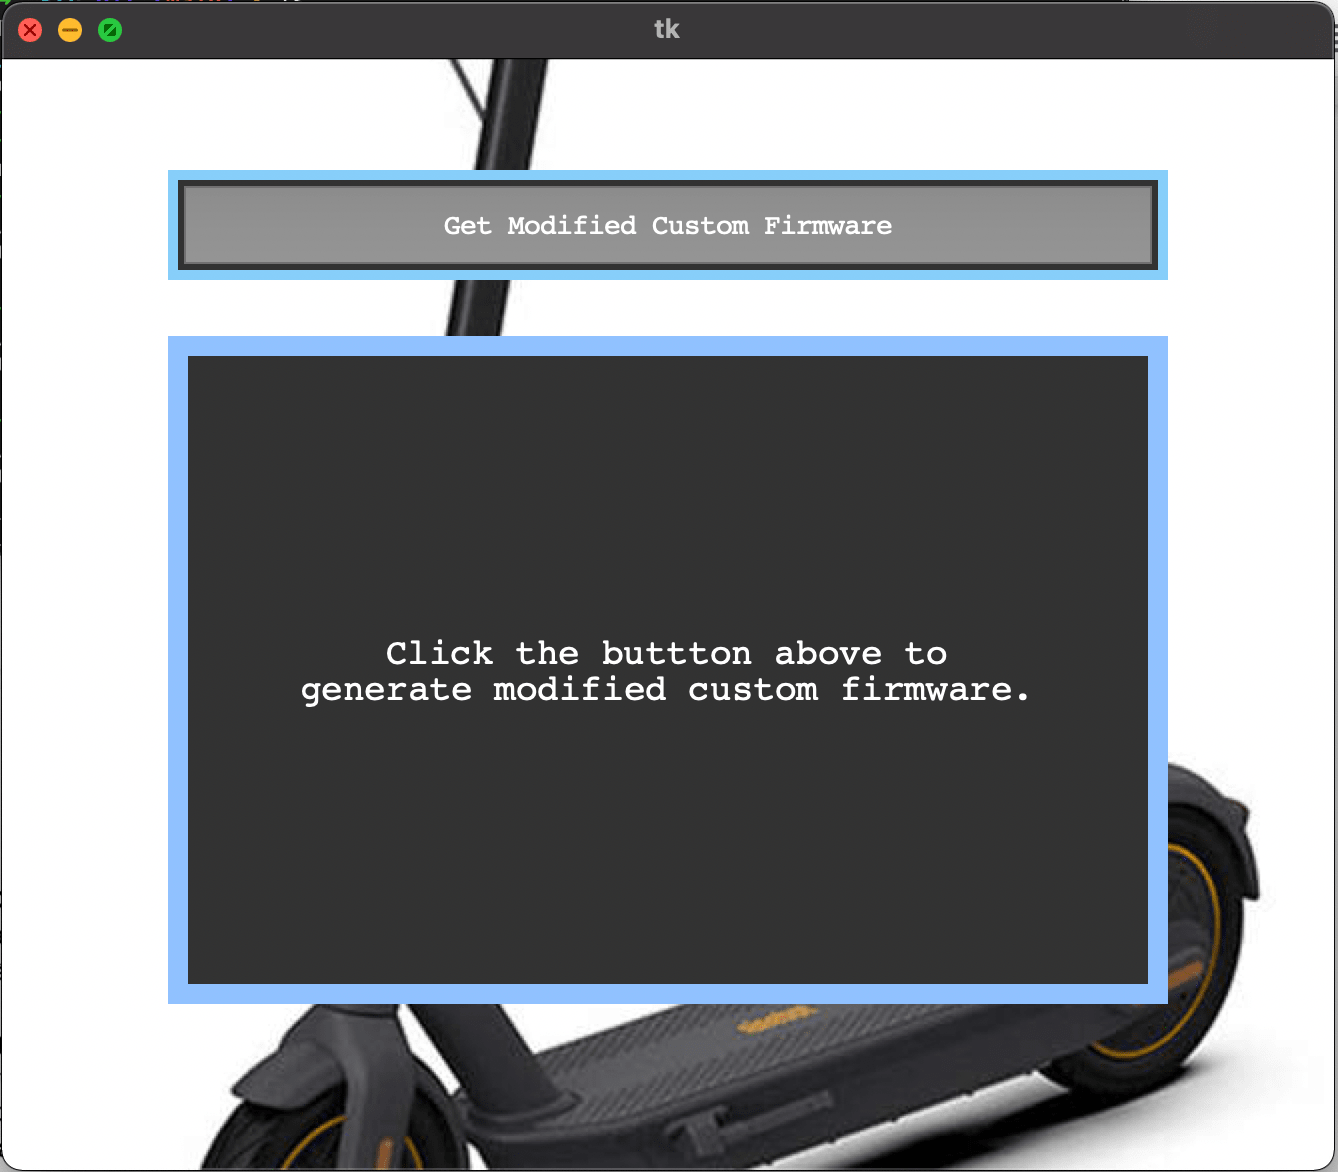
\includegraphics[width=.9\linewidth]{images/gui1.png}
\end{minipage}%
\begin{minipage}{.5\textwidth}
  \centering
  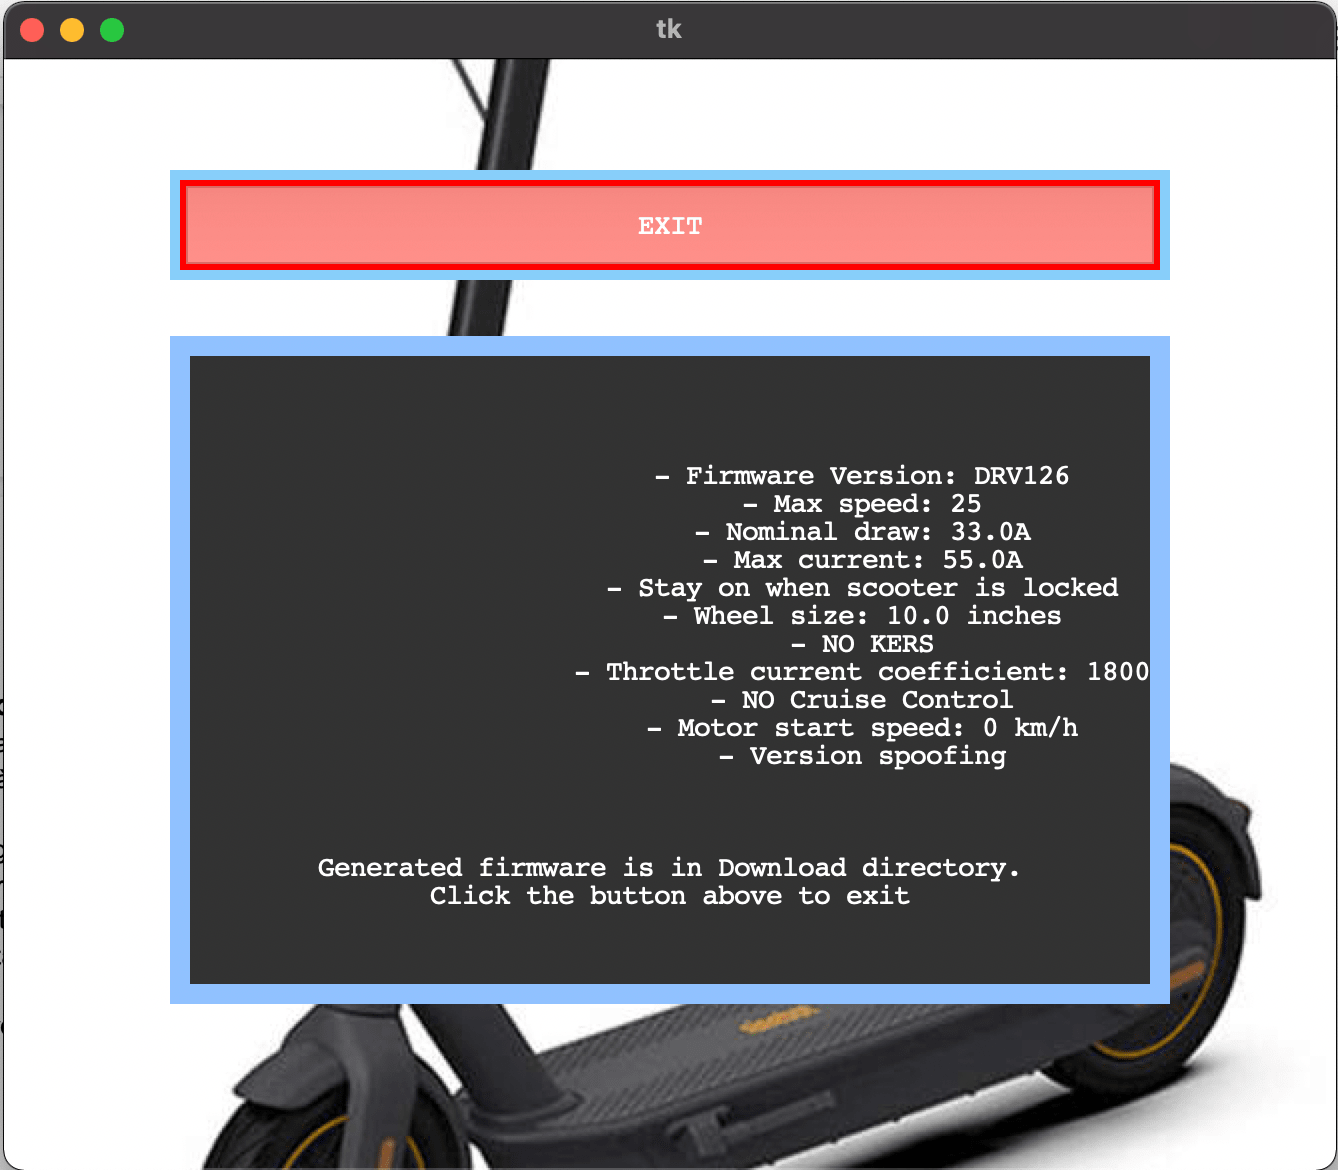
\includegraphics[width=.9\linewidth]{images/gui2.png}
\end{minipage}
\label{fig:test2}
\captionof{figure}{Graphical interface of the firmware generator}
\end{figure}

\noindent At the end of the guided firmware generation process, by clicking on the "EXIT" button the firmware will be saved in the download folder in .zip format. This archive will contain the firmware binary file to be flashed and a text file describing the modified parameters.\\
\noindent To flash the firmware on the electric scooter, just use one of the third party software available on AppStore or PlayStore and start the test. In our case, an iOS app still under development called Scooter Companion was used. In figure \ref{fig:scooter_comp_app}, a screenshot of the app is shown.
\begin{figure}[!htp]
    \centering
    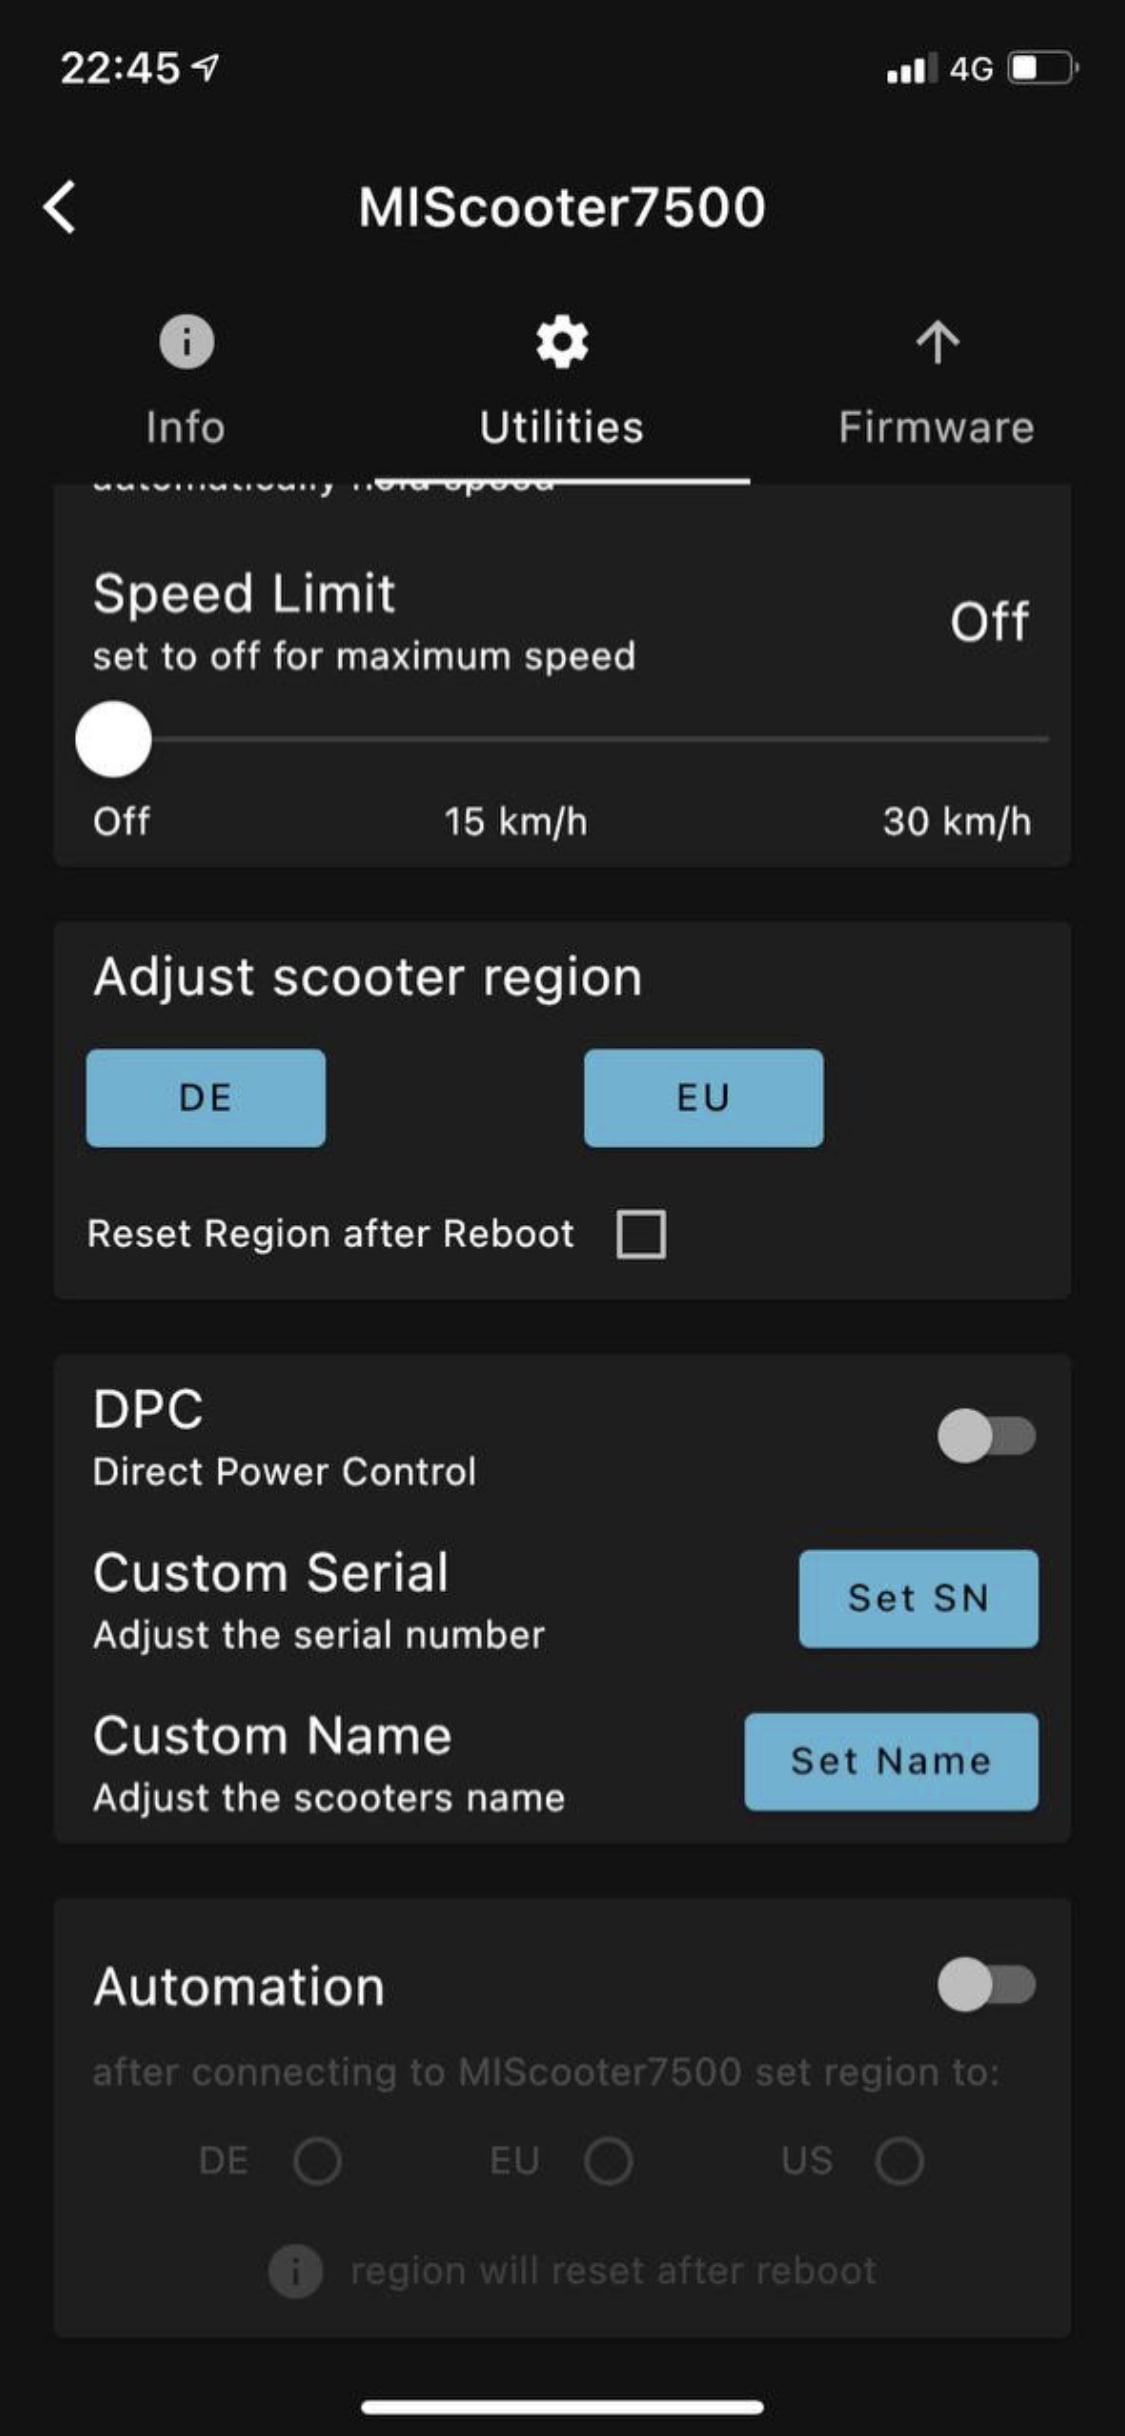
\includegraphics[width = .26\textwidth]{images/scooter_companion.jpeg}
    \caption{Scooter Companion Application}
    \label{fig:scooter_comp_app}
\end{figure}

\chapter{First Assembly and Experimental Results}
In this chapter we will show the various ways in which the mechanical coupling between the two parts has been provided, ie between the wheelchair and the electric scooter. Specifically, two main ways of interconnecting the parts have been identified, but each of them has advantages and disadvantages that we will also illustrate through images showing the type of assembly. In both cases, the support that allows the connection between the two parts is the same therefore the use of one mode over another does not affect the components and is at the discretion of the end user. More specifically, a support has been created to be installed at the base of the wheelchair structure near the rear wheels, thus becoming an integral part of the wheelchair structure. A movable component is added to this support which, by means of a knob, allows the electric scooter to be fixed to the aforementioned support.\\
Specifically, three knobs were used connected to three respective threaded rods and three 3D printed nylon anti-vibration pads. The threaded bars have been cut to size and, through a joint in the part that connects them to the anti-vibration mounts, allows any type of electric scooter to be kept firmly on the support with respect to the longitudinal and lateral movements produced by acceleration, braking and steering phenomena. Furthermore, the knob placed in a horizontal position with respect to the ground allows to raise the position of the front wheels of the wheelchair which, in both assembly modes, would create problems of a kinematic nature. In this sense they are "disabled" in their functionality and therefore the movement of the wheelchair will be subject only to the traction and steering imposed by the electric scooter. In addition, by means of a steel hinge, the mobile part connected to the support allows the electric scooter to enter under the wheelchair without it having to be lifted or moved. In the following, images relating to the various parts of the coupling and the components used will be shown.

\newpage
\begin{figure}[!htp]
    \centering
    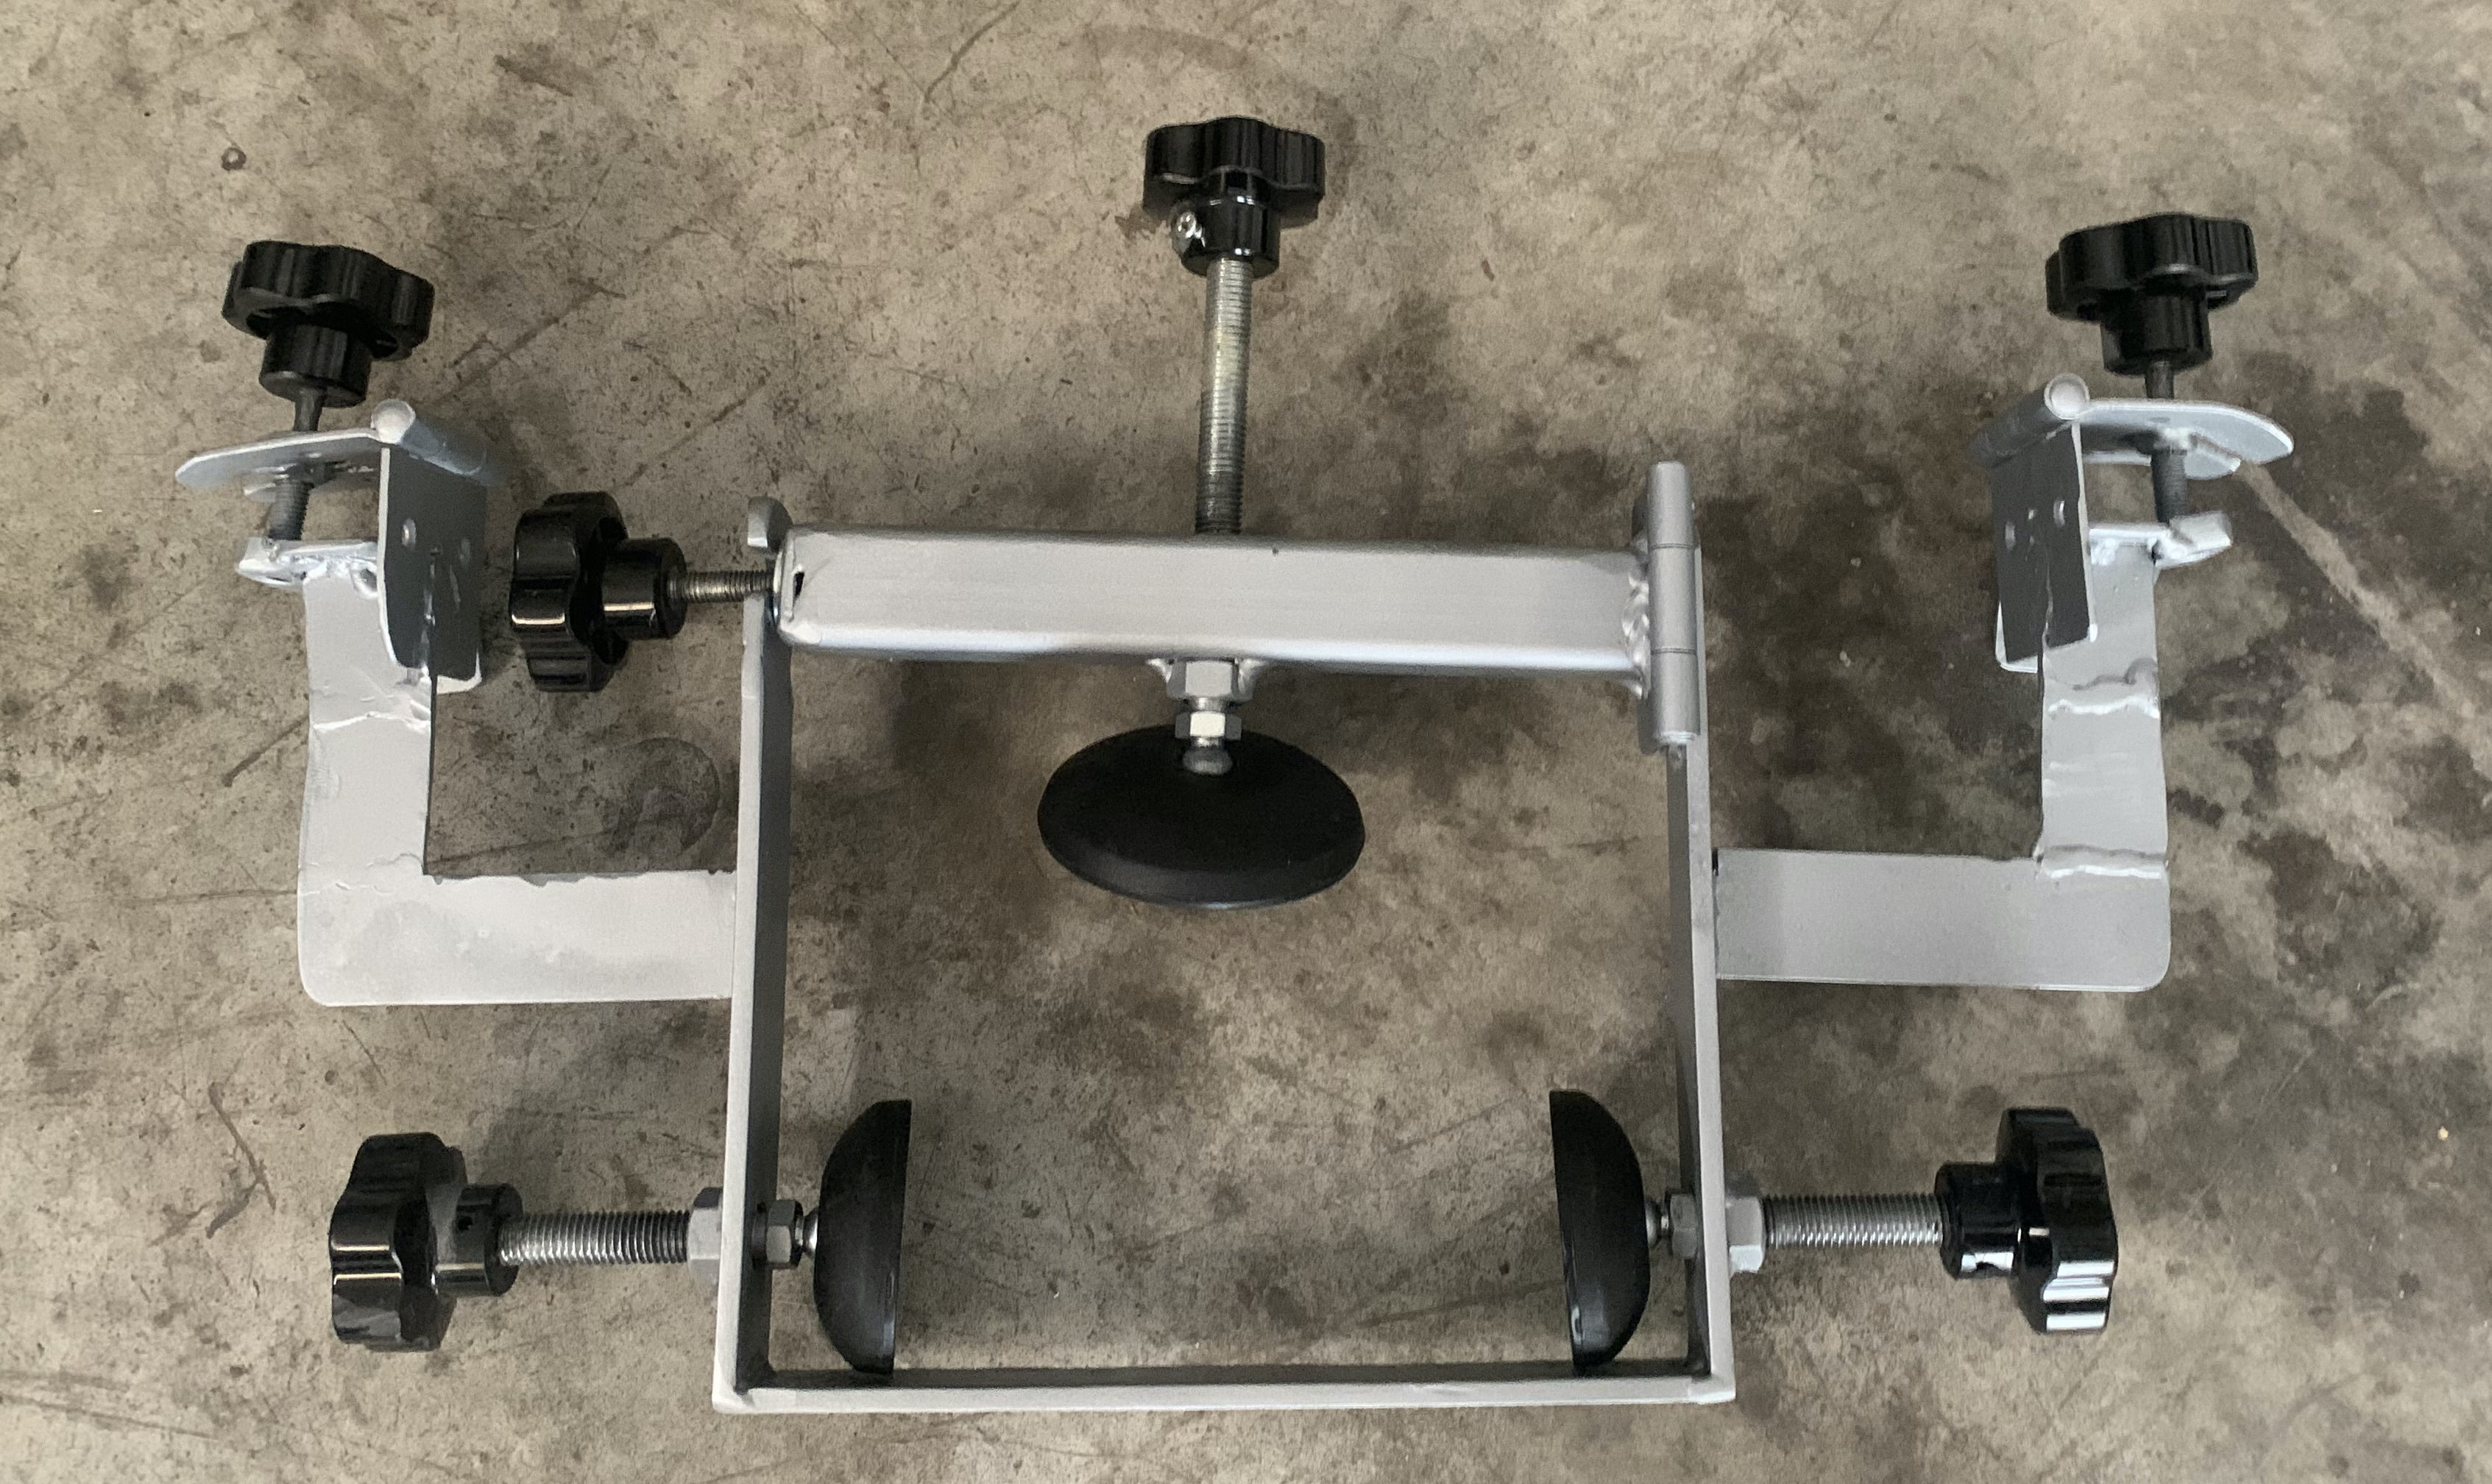
\includegraphics[width=\textwidth]{images/finished_project/IMG_3684.jpg}
    % \caption{Latest bracket prototype}
    % \label{fig:latest_bracket_prototype}
\end{figure}

\begin{figure}[!htp]
    \begin{minipage}[t]{.5\textwidth}
    \centering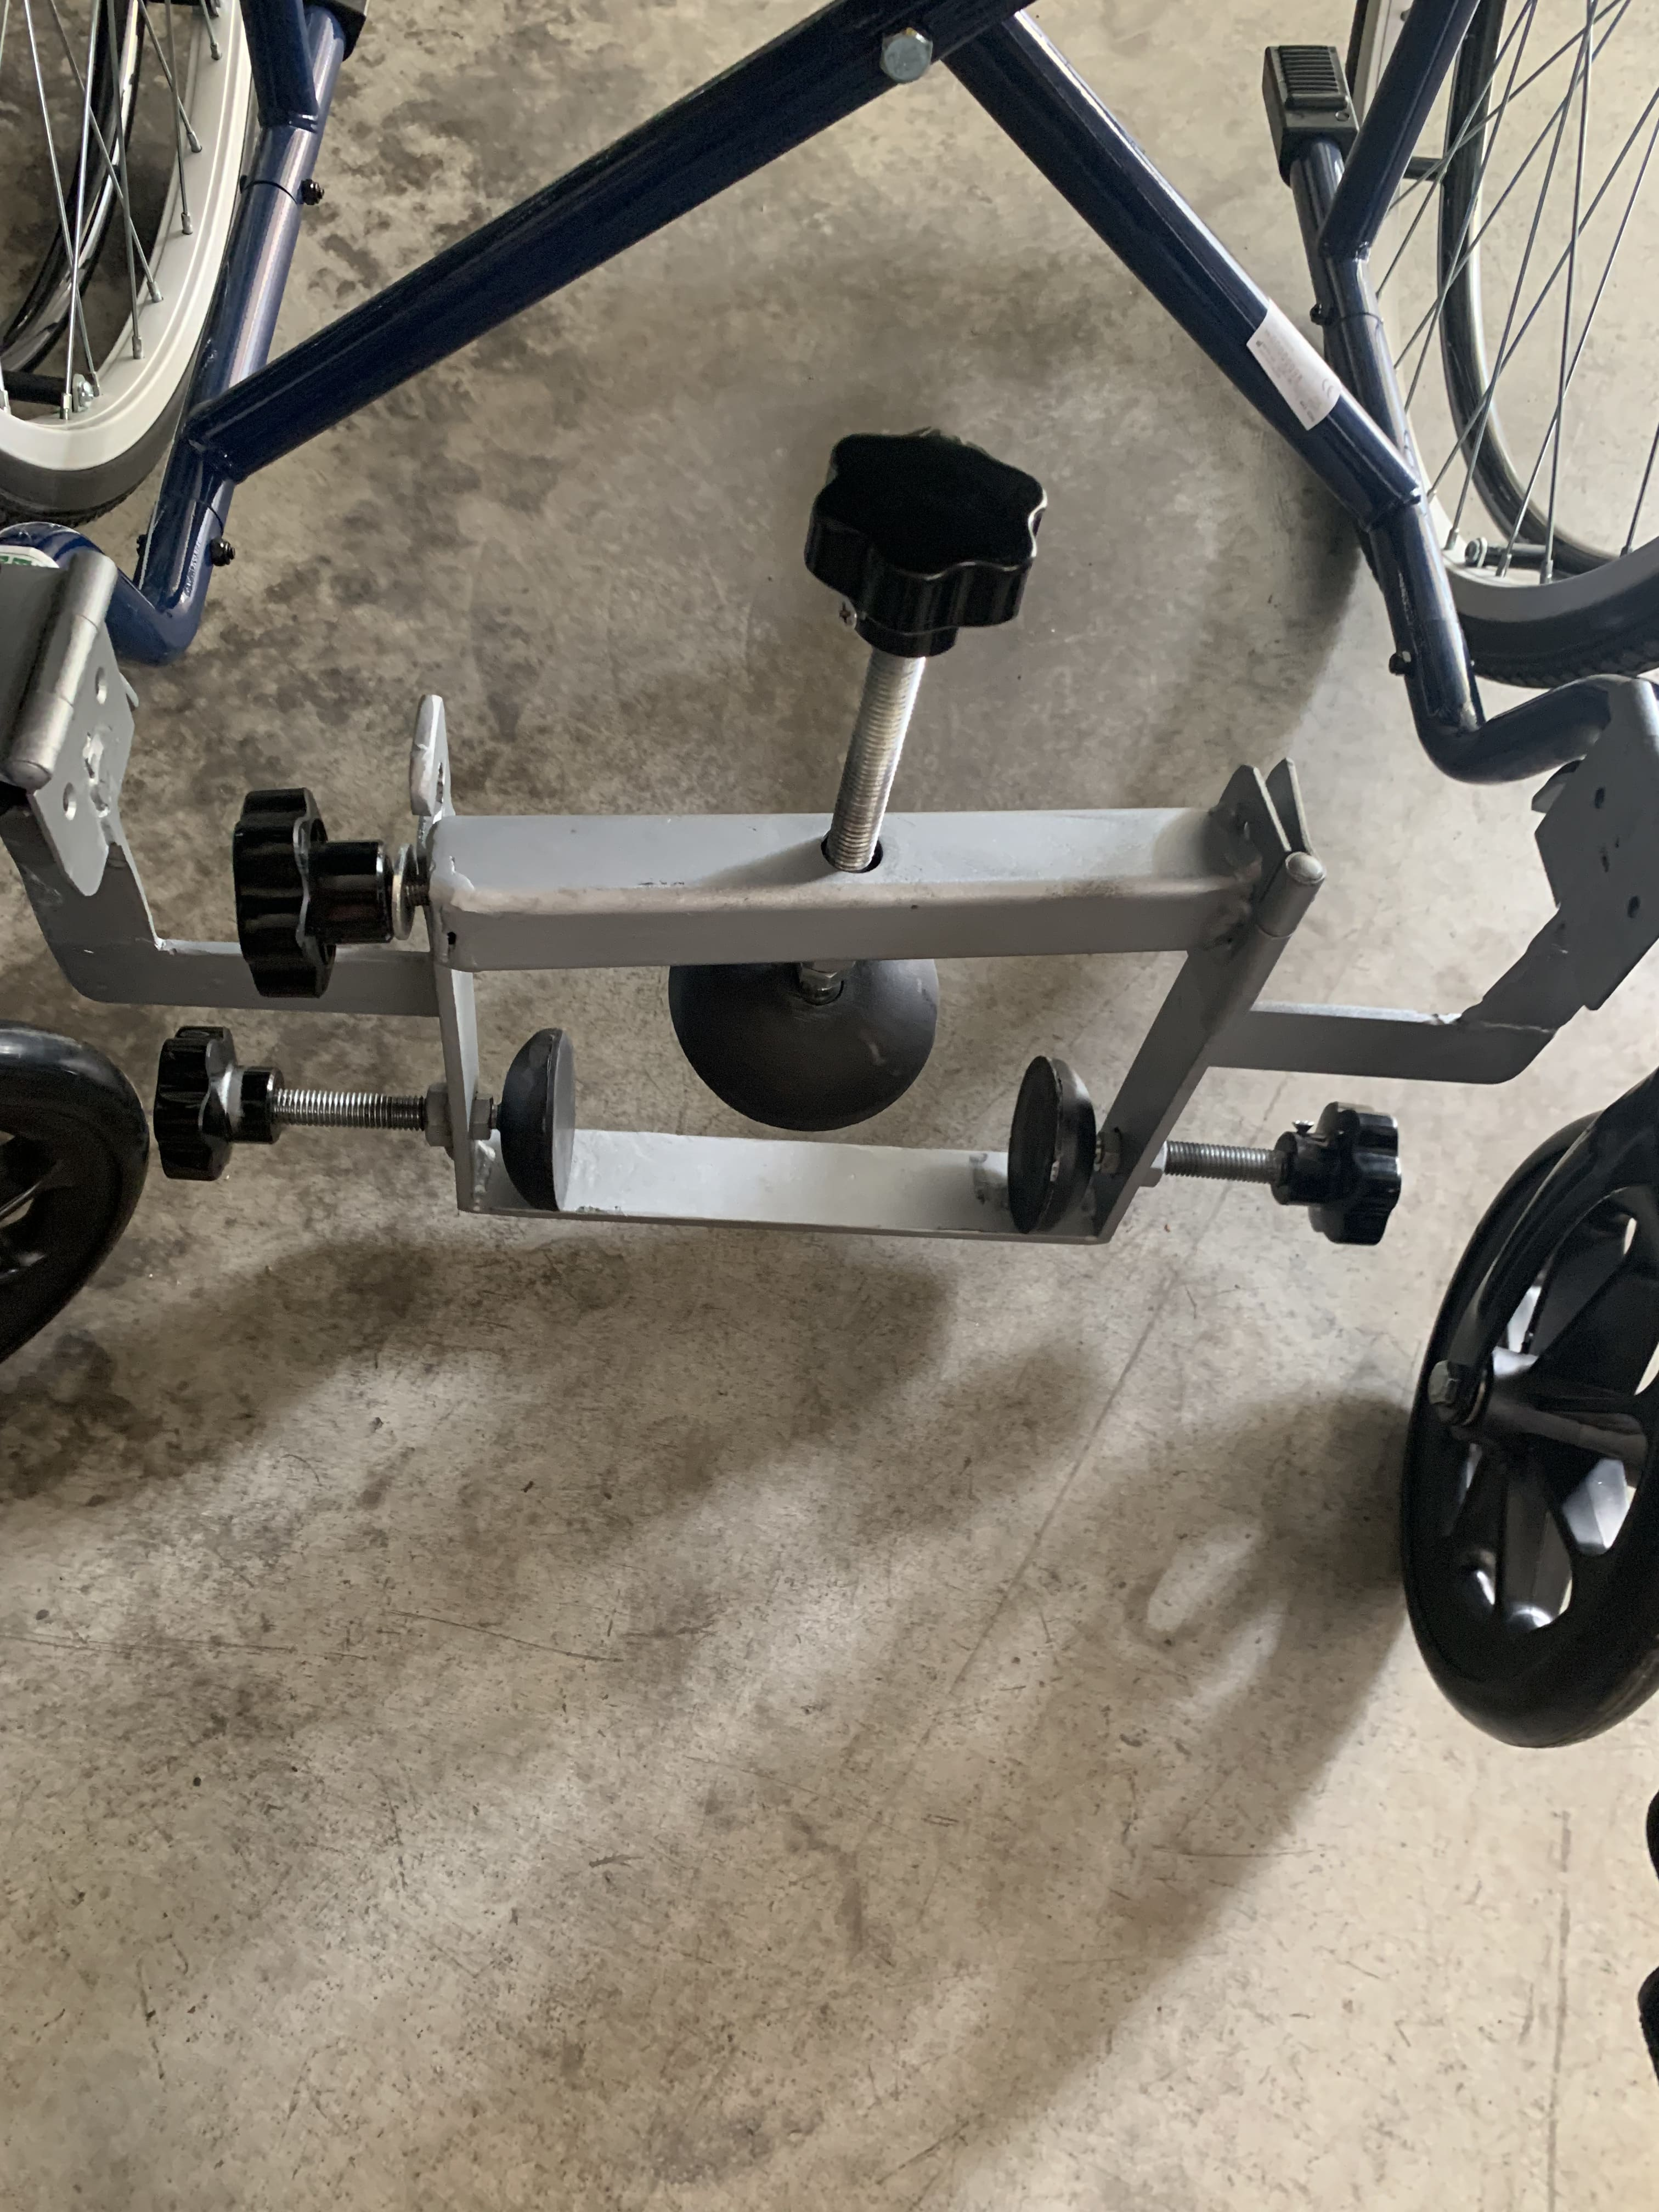
\includegraphics[width=.95\textwidth]{images/finished_project/IMG_3766.jpg}
    \end{minipage}
    \begin{minipage}[t]{.5\textwidth}
    \centering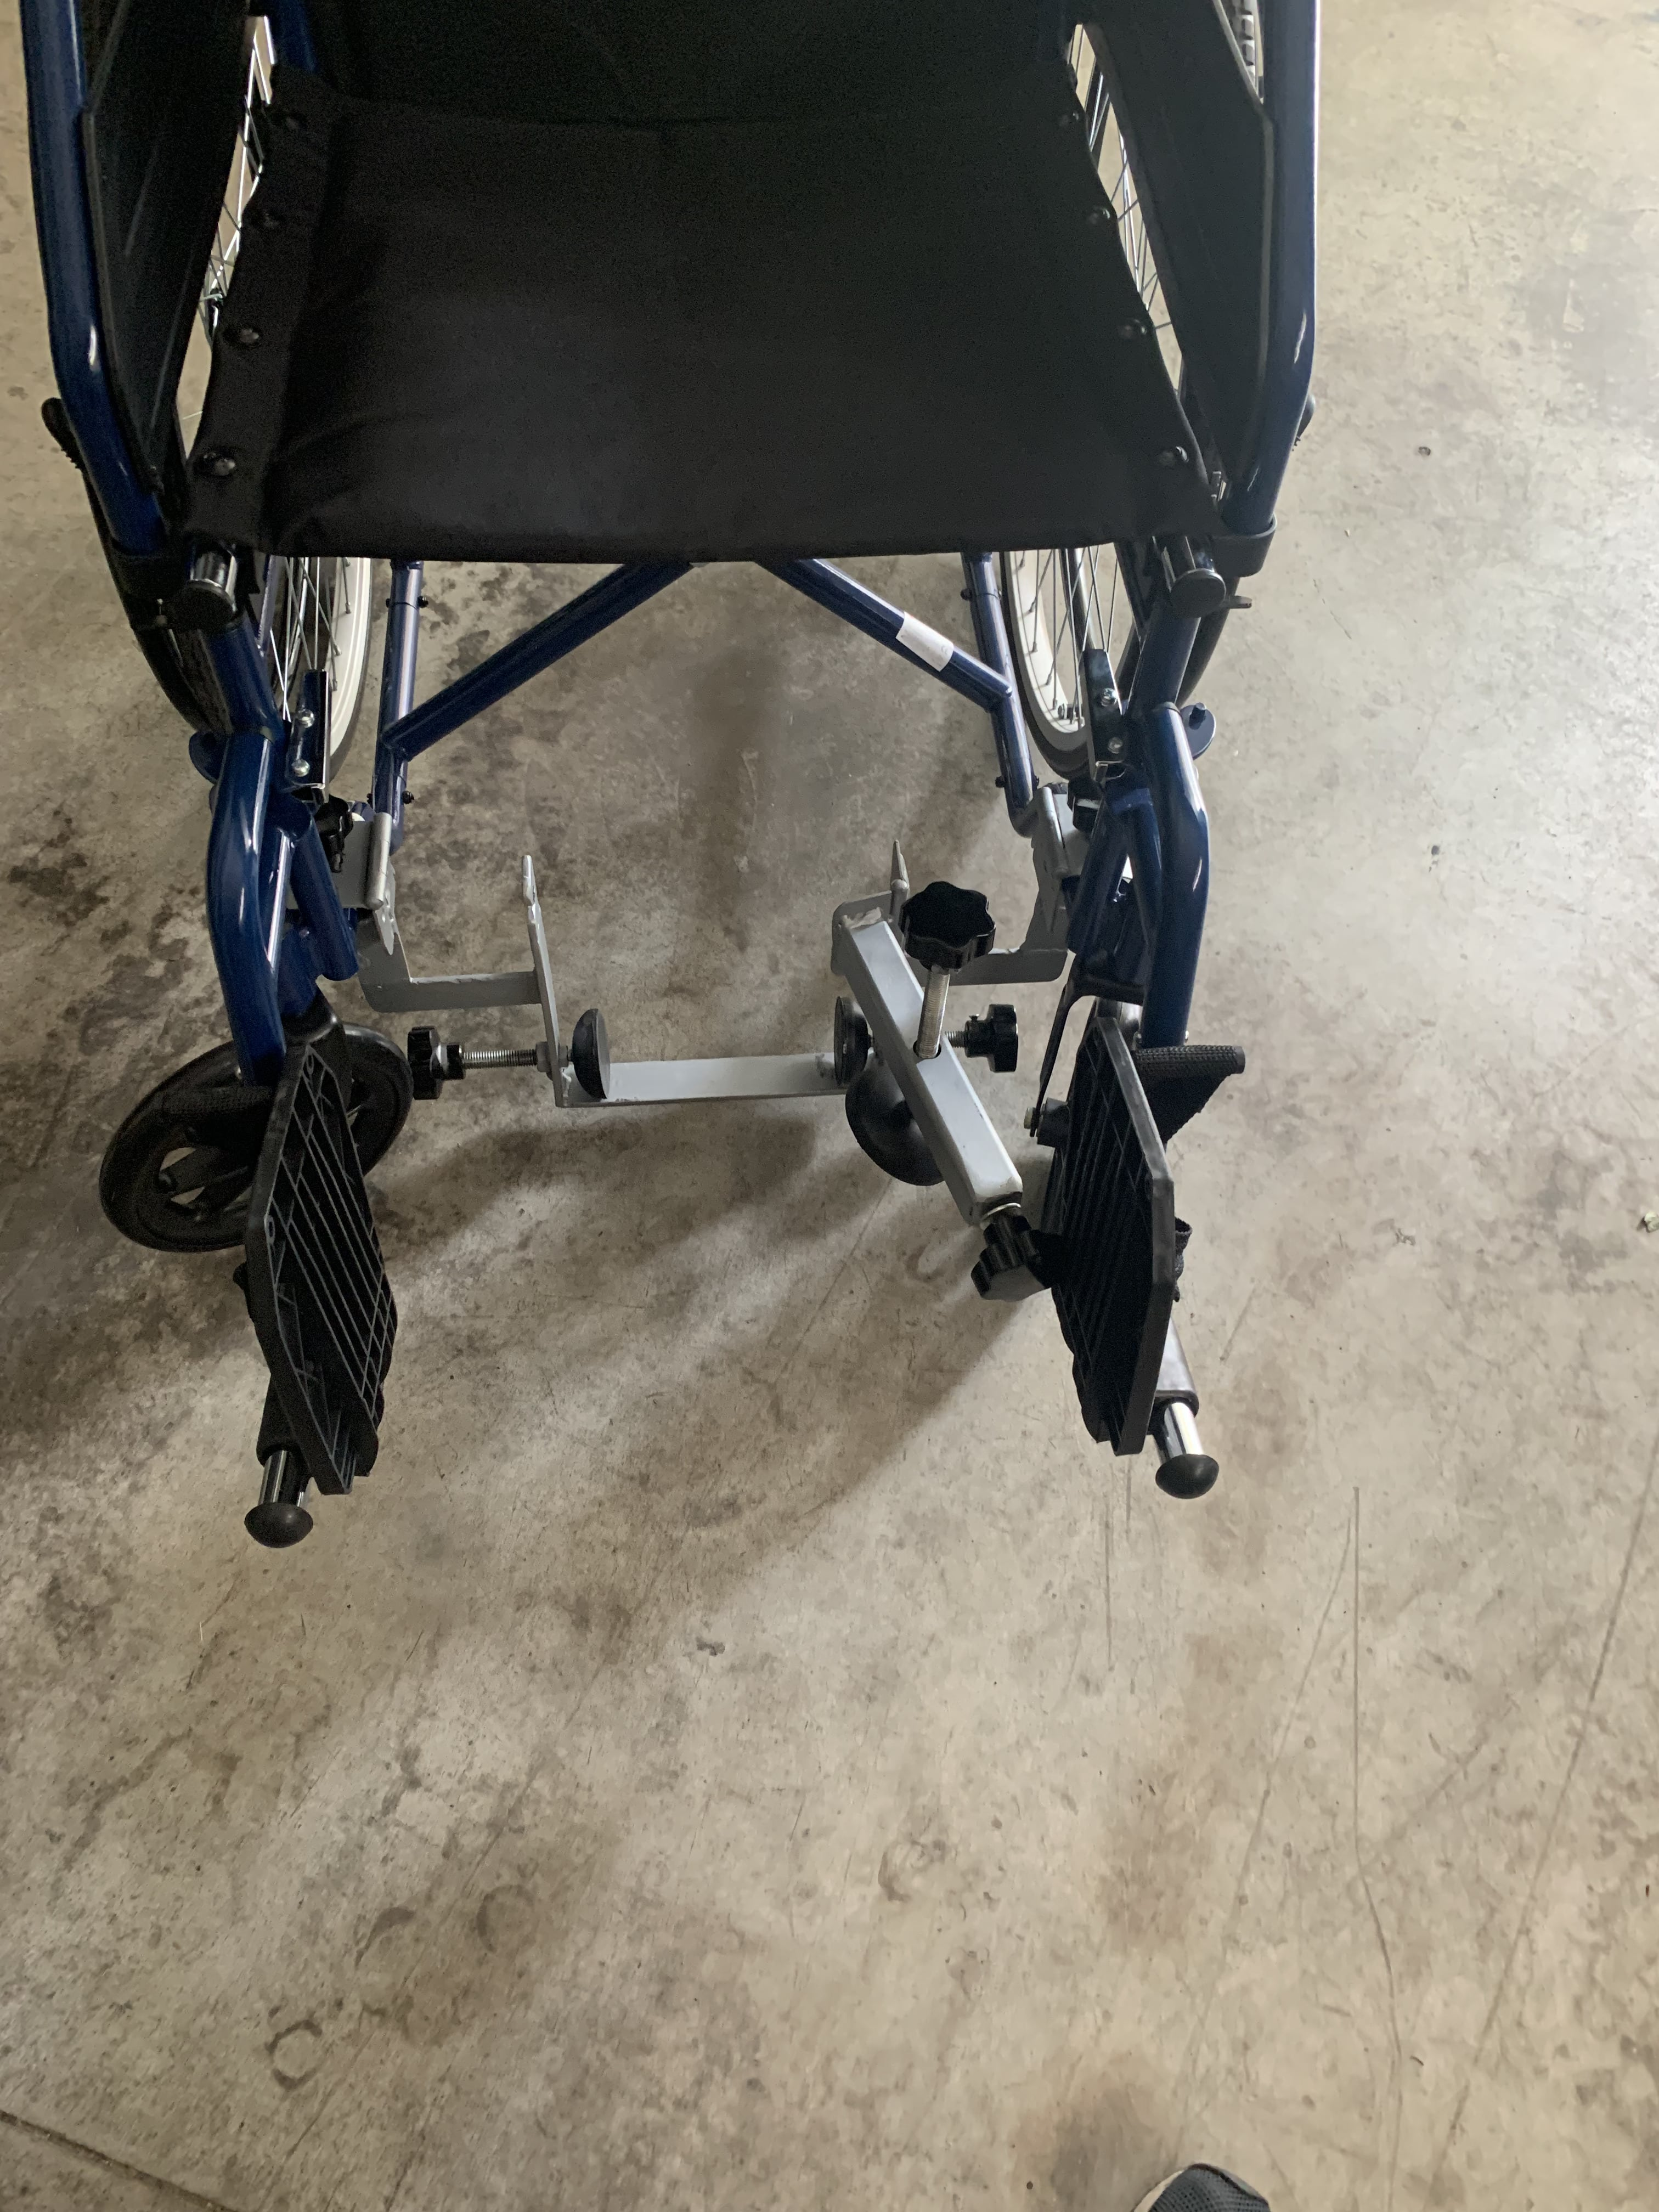
\includegraphics[width=.95\textwidth]{images/finished_project/IMG_3765.jpg}
    \end{minipage}
    \caption{Bracket mounted on the wheelchair}
    \label{fig:brack_mounted}
\end{figure}

% \begin{center}
% Fai un progetto autocad con le misure precise e metti qui il pdf
% \end{center}
Furthermore, since electric scooters do not have reverse gear at the level of the electric motor, it is necessary to ensure that this is still done even by those with disabilities.In this sense, the structure we have built does not interfere in any way with the user's ability to go backwards as he would have done with a wheelchair not equipped with the scooter. Specifically, by acting on the rear wheels of the wheelchair and making the steering using the handlebar of the electric scooter, it is possible to reverse without any effort without the e-scooter being an obstacle in carrying out these actions.

\section{First assembly method}
The first assembly method requires that the rear wheel of the electric scooter is located before the "x" structure, that is the one that allows the wheelchair to be folded. The use of this mode requires that the steering wheel of the electric scooter is folded because otherwise it would be too far from the wheelchair seat. In this sense, the use of the folded steering allows the user to enjoy a wide view and at the same time to carry out steering maneuvers easily and without fatigue. On the other hand, however, the turning radius is considerably reduced, ie by about 20\% of the steering wheel of the electric scooter, which in fact reduces the steering capacity of the electric scooter. Some images related to this assembly method and its use will be shown below.

\begin{figure}[!htp]
    \centering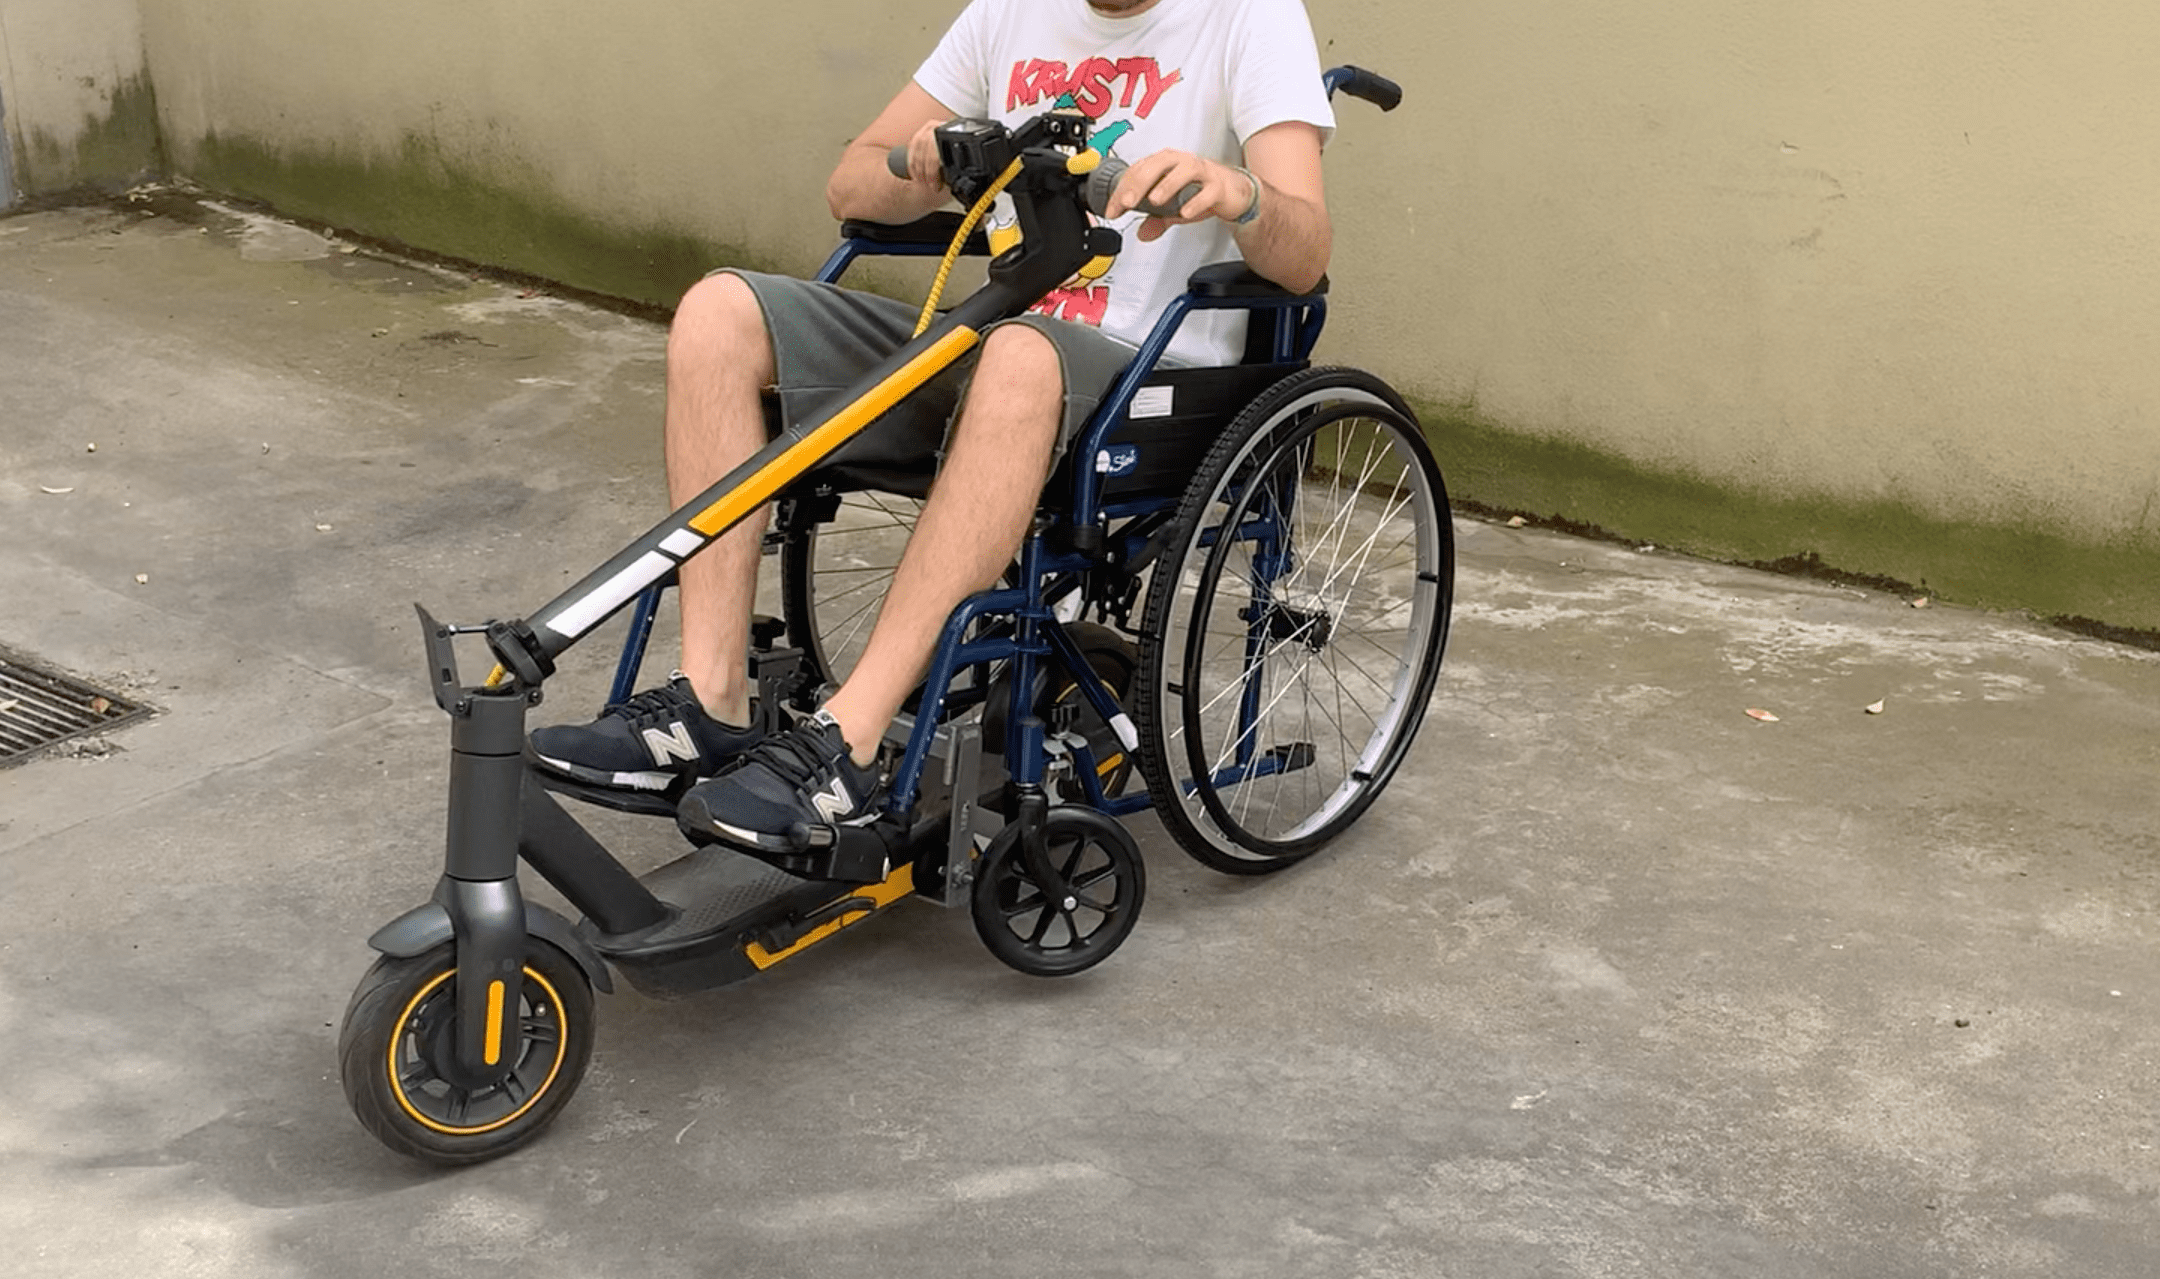
\includegraphics[width=.9\textwidth]{images/finished_project/IMG_2332-2.png}
    % \newpage
    \centering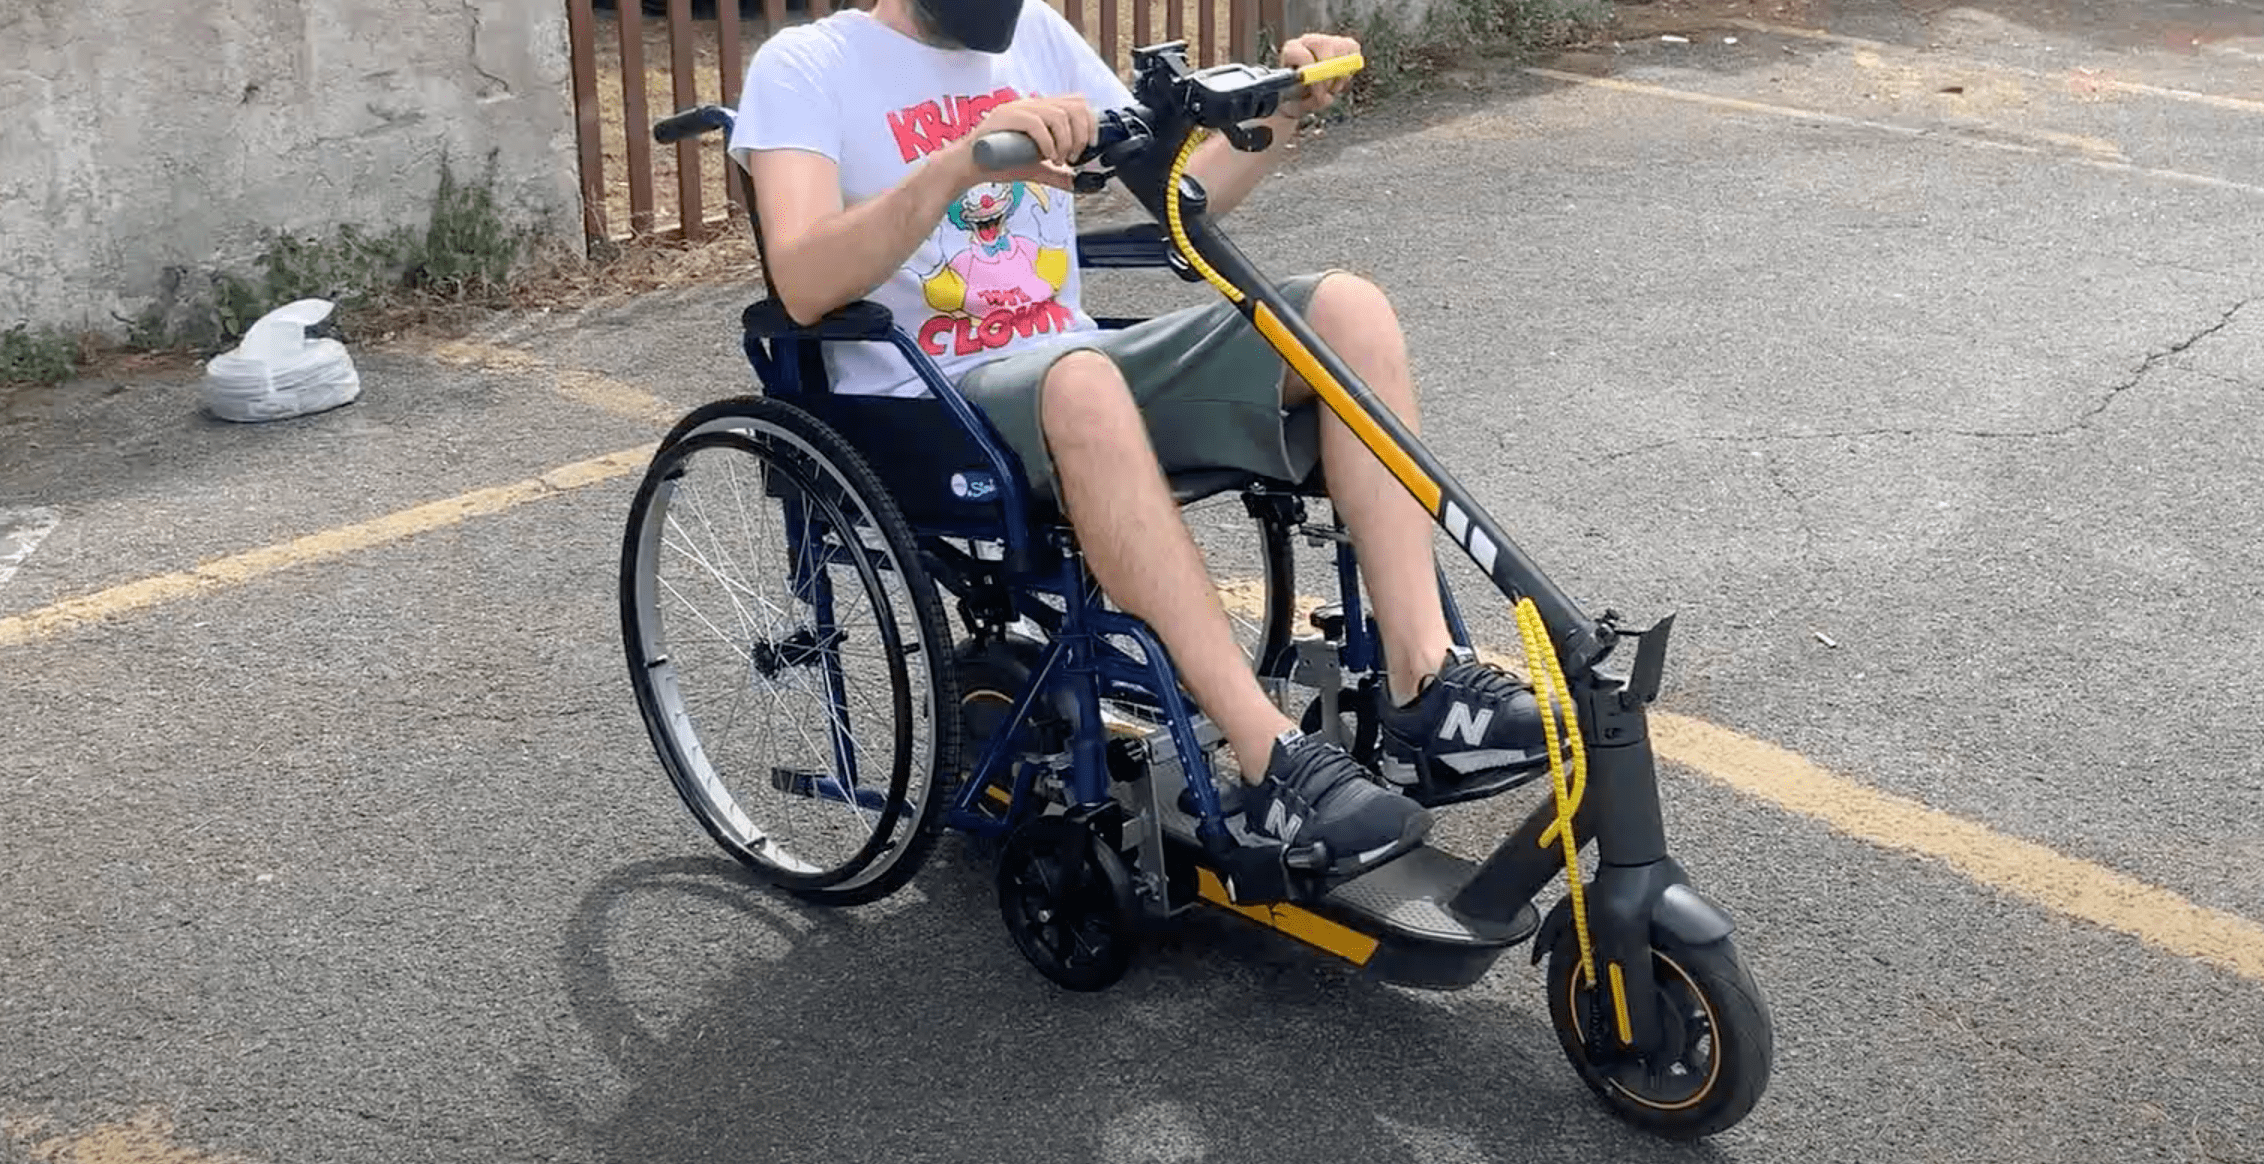
\includegraphics[width=.9\textwidth]{images/finished_project/IMG_2334-2.png}
    \caption{First assembly method}
    \label{fig:first_ass}
\end{figure}

\noindent In light of this problem, a further method of assembly has therefore been envisaged, although this is the one that has the most advantages at the current stage of development.

\section{Second assembly method}
The second assembly method foresees that the position of the rear wheel is located before the “x” structure of the wheelchair described above. In this case, unlike the previous driving mode, the handlebar is located much closer to the user so it is not necessary to use it folded and this allows you to take full advantage of the turning radius of the electric scooter. On the other hand, however, this configuration reduces the end user's field of vision since the steering will be located at a higher height than the user's shoulders. This is because the electric scooter is designed to be used in an upright position. Obviously this problem would be solved when using an electric scooter with telescopic steering, therefore able to support different heights for the steering.\\

\noindent Some images related to this assembly method and its use will be shown below.

\begin{figure}[!htp]
    \begin{minipage}[t]{.5\textwidth}
    \centering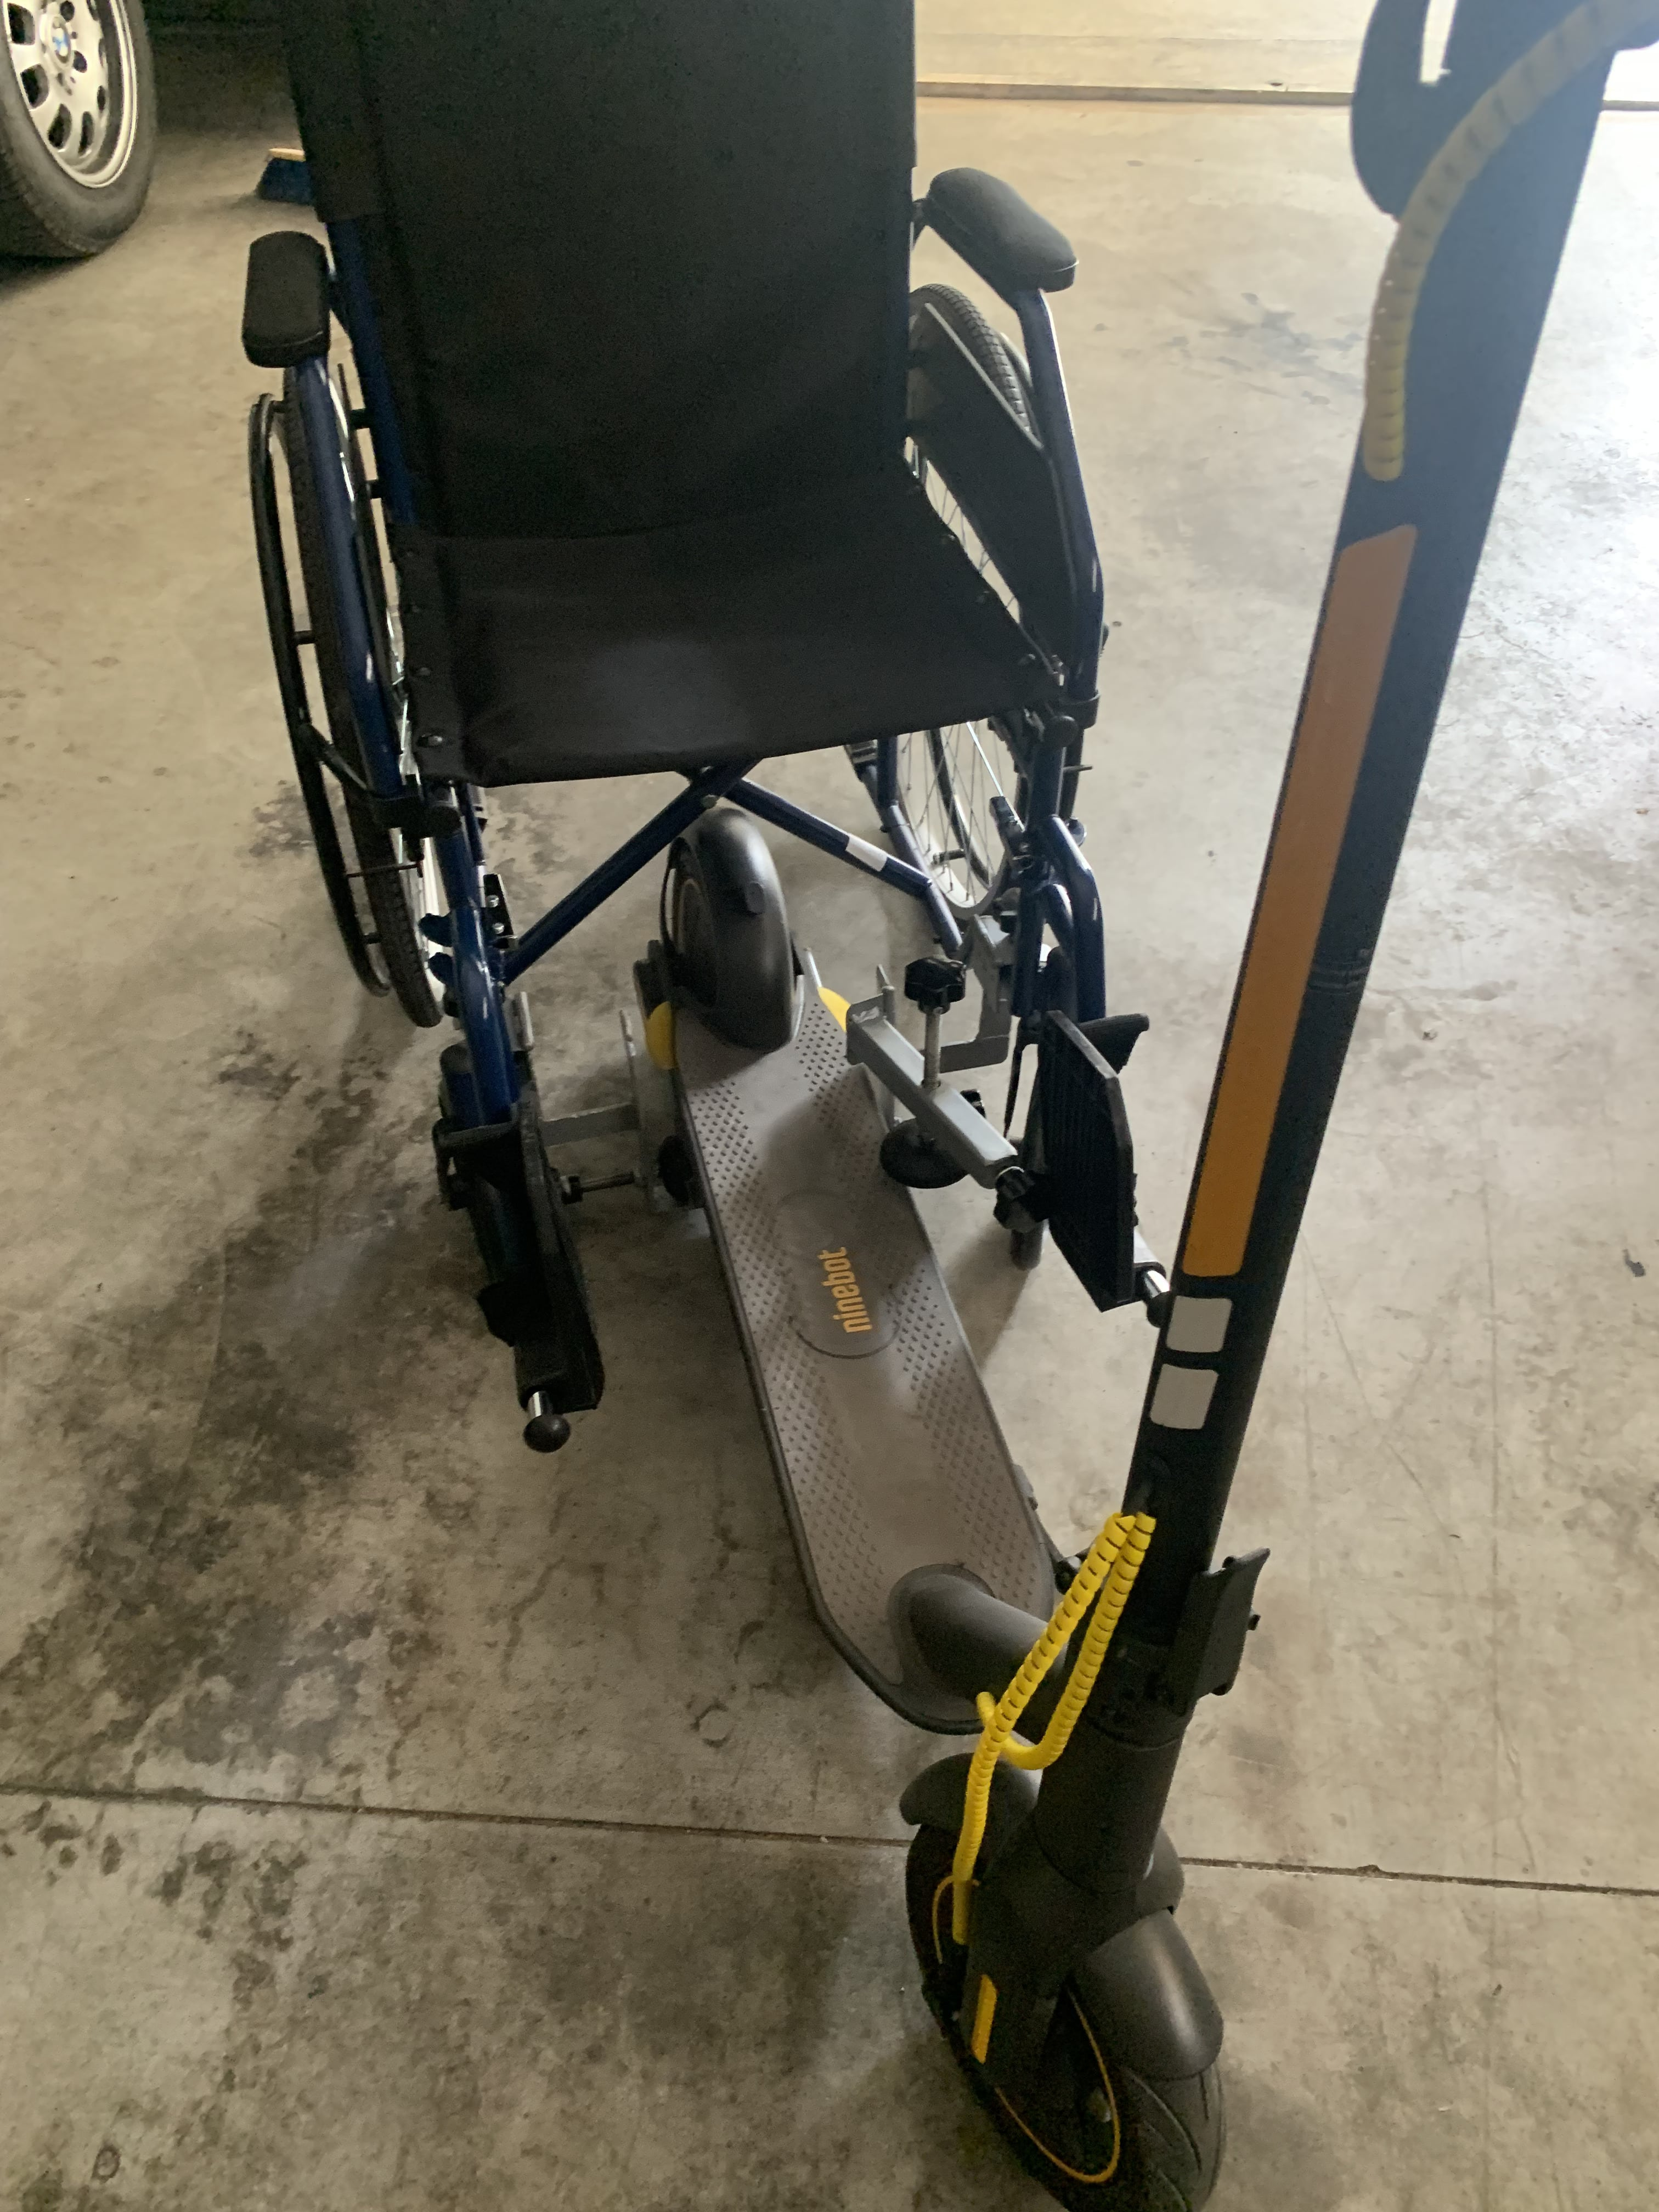
\includegraphics[width=.95\textwidth]{images/finished_project/IMG_3762.jpg}
    \end{minipage}
    \begin{minipage}[t]{.5\textwidth}
    \centering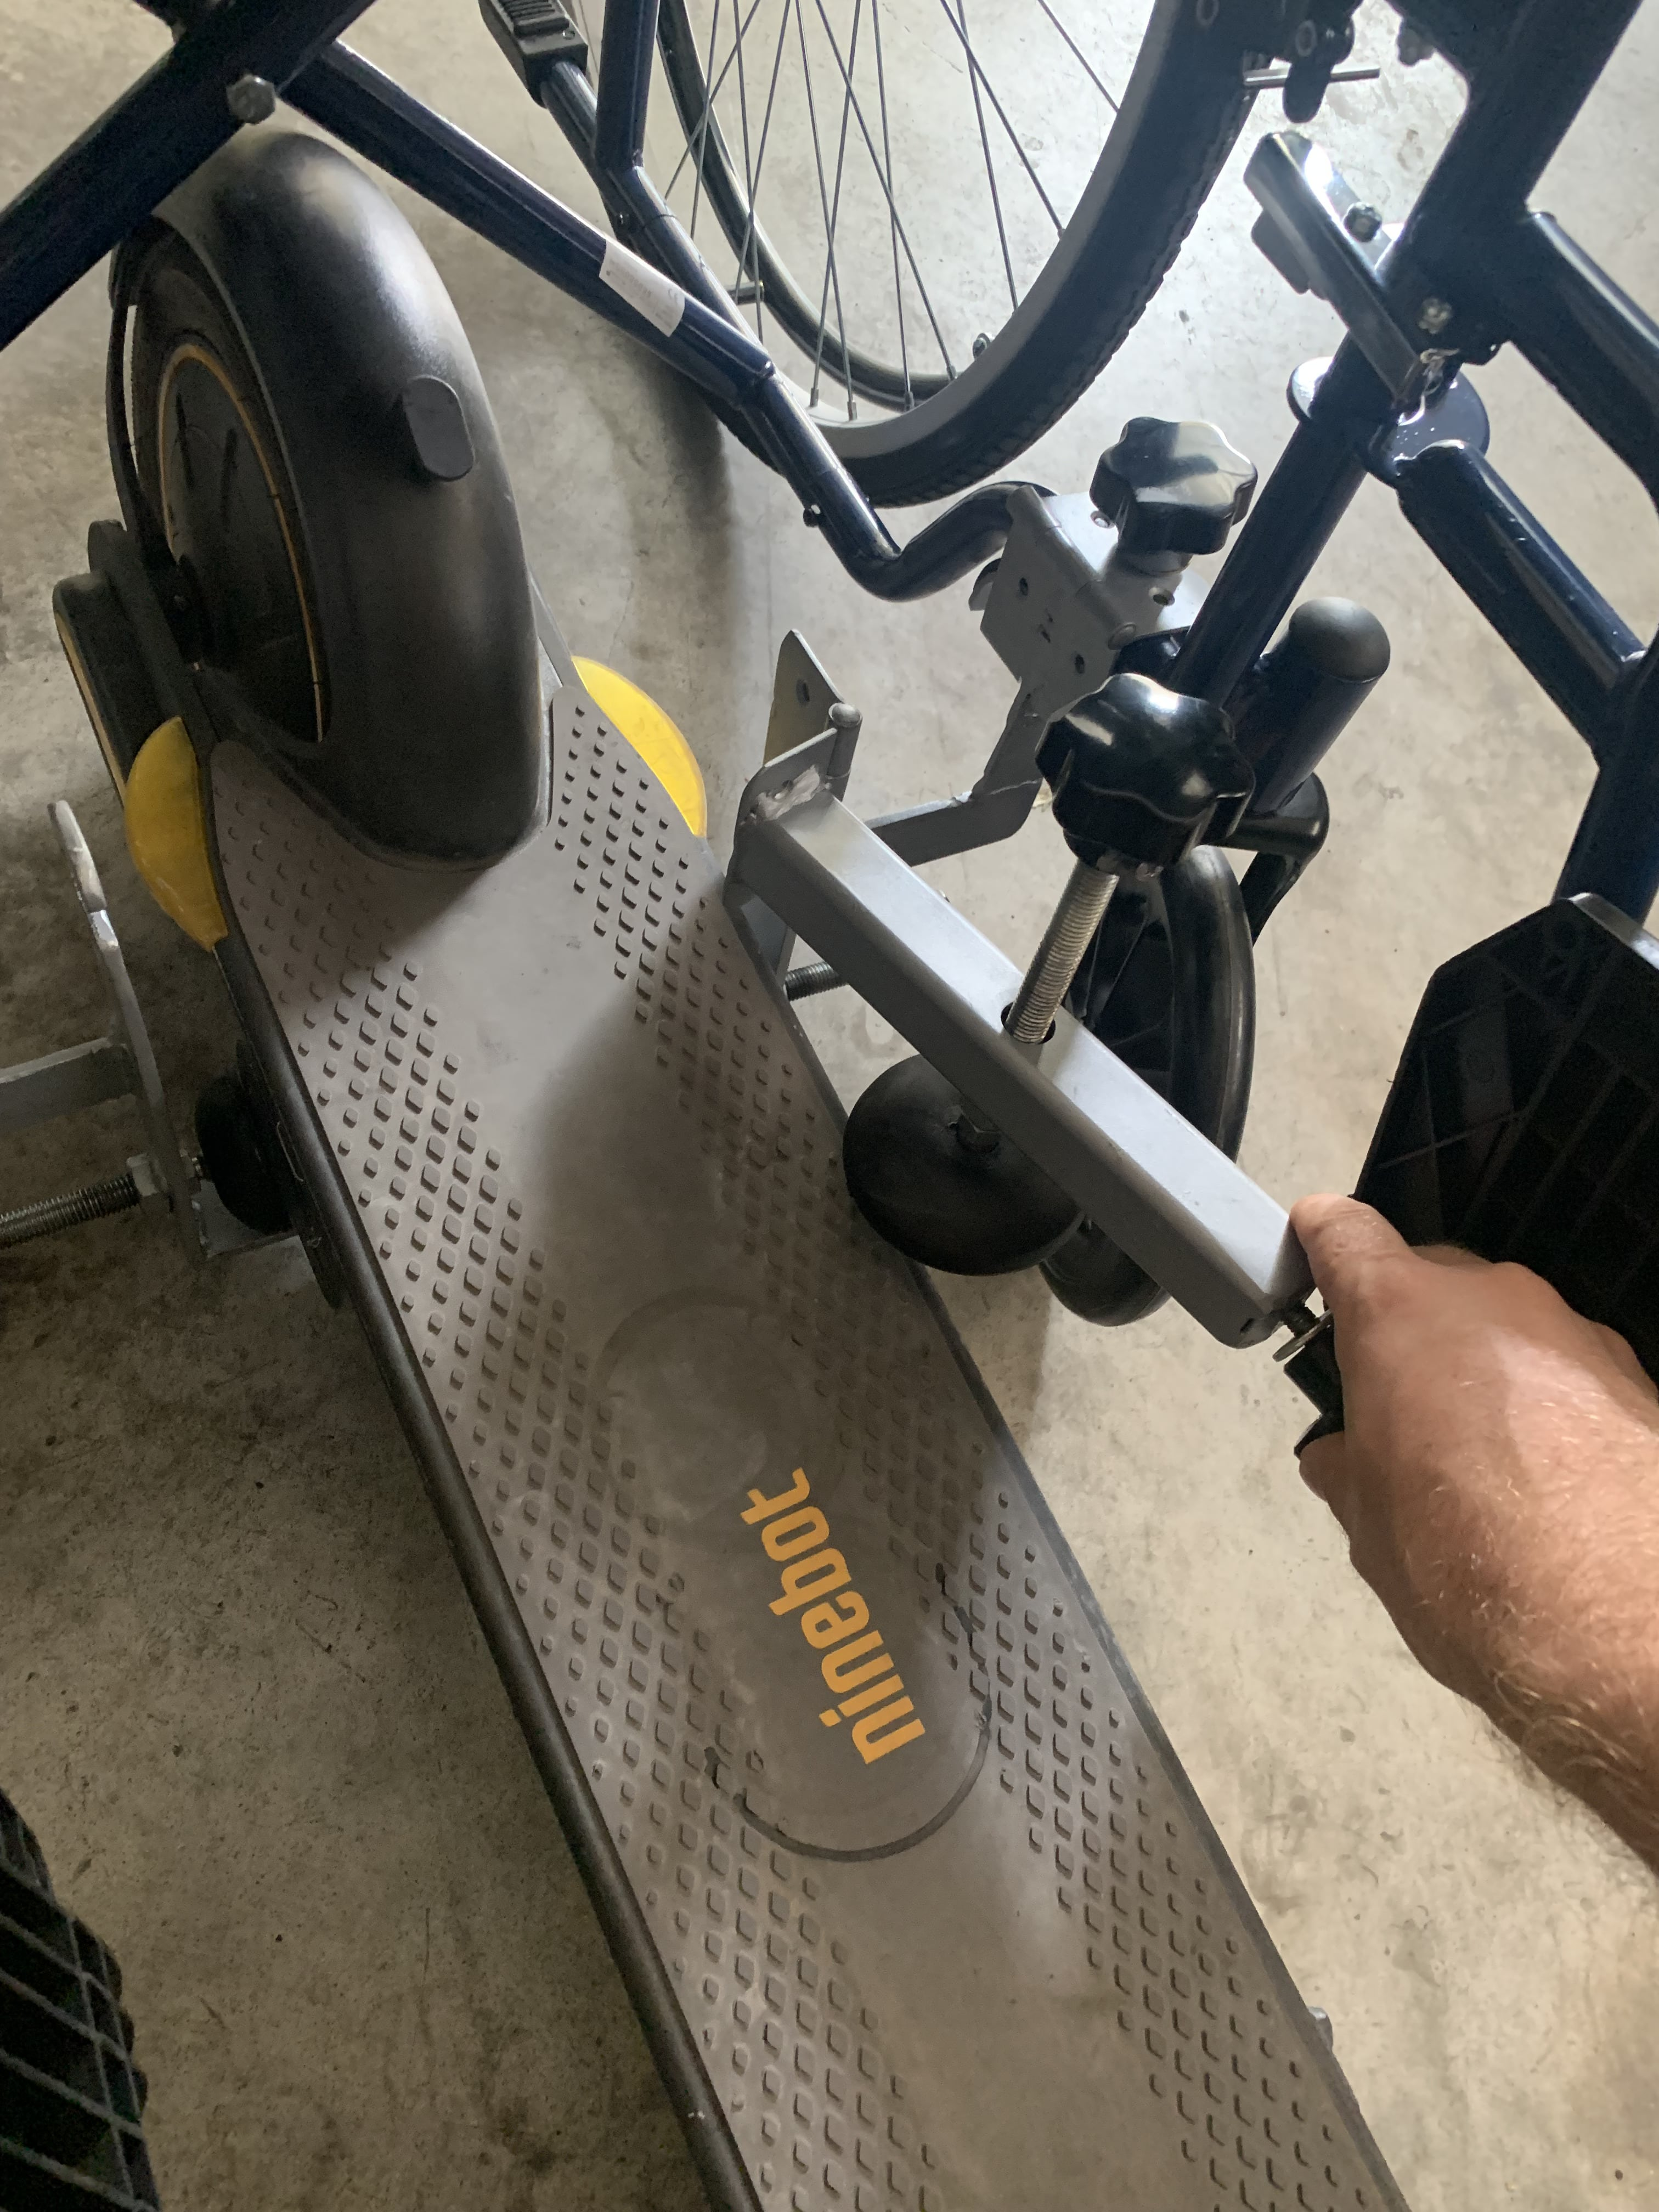
\includegraphics[width=.95\textwidth]{images/finished_project/IMG_3763.jpg}
    \end{minipage}
    % \caption{Bracket mounted on the wheelchair}
    % \label{fig:second_ass_method1}
\end{figure}

\newpage
\begin{figure}[!htp]
    \centering
    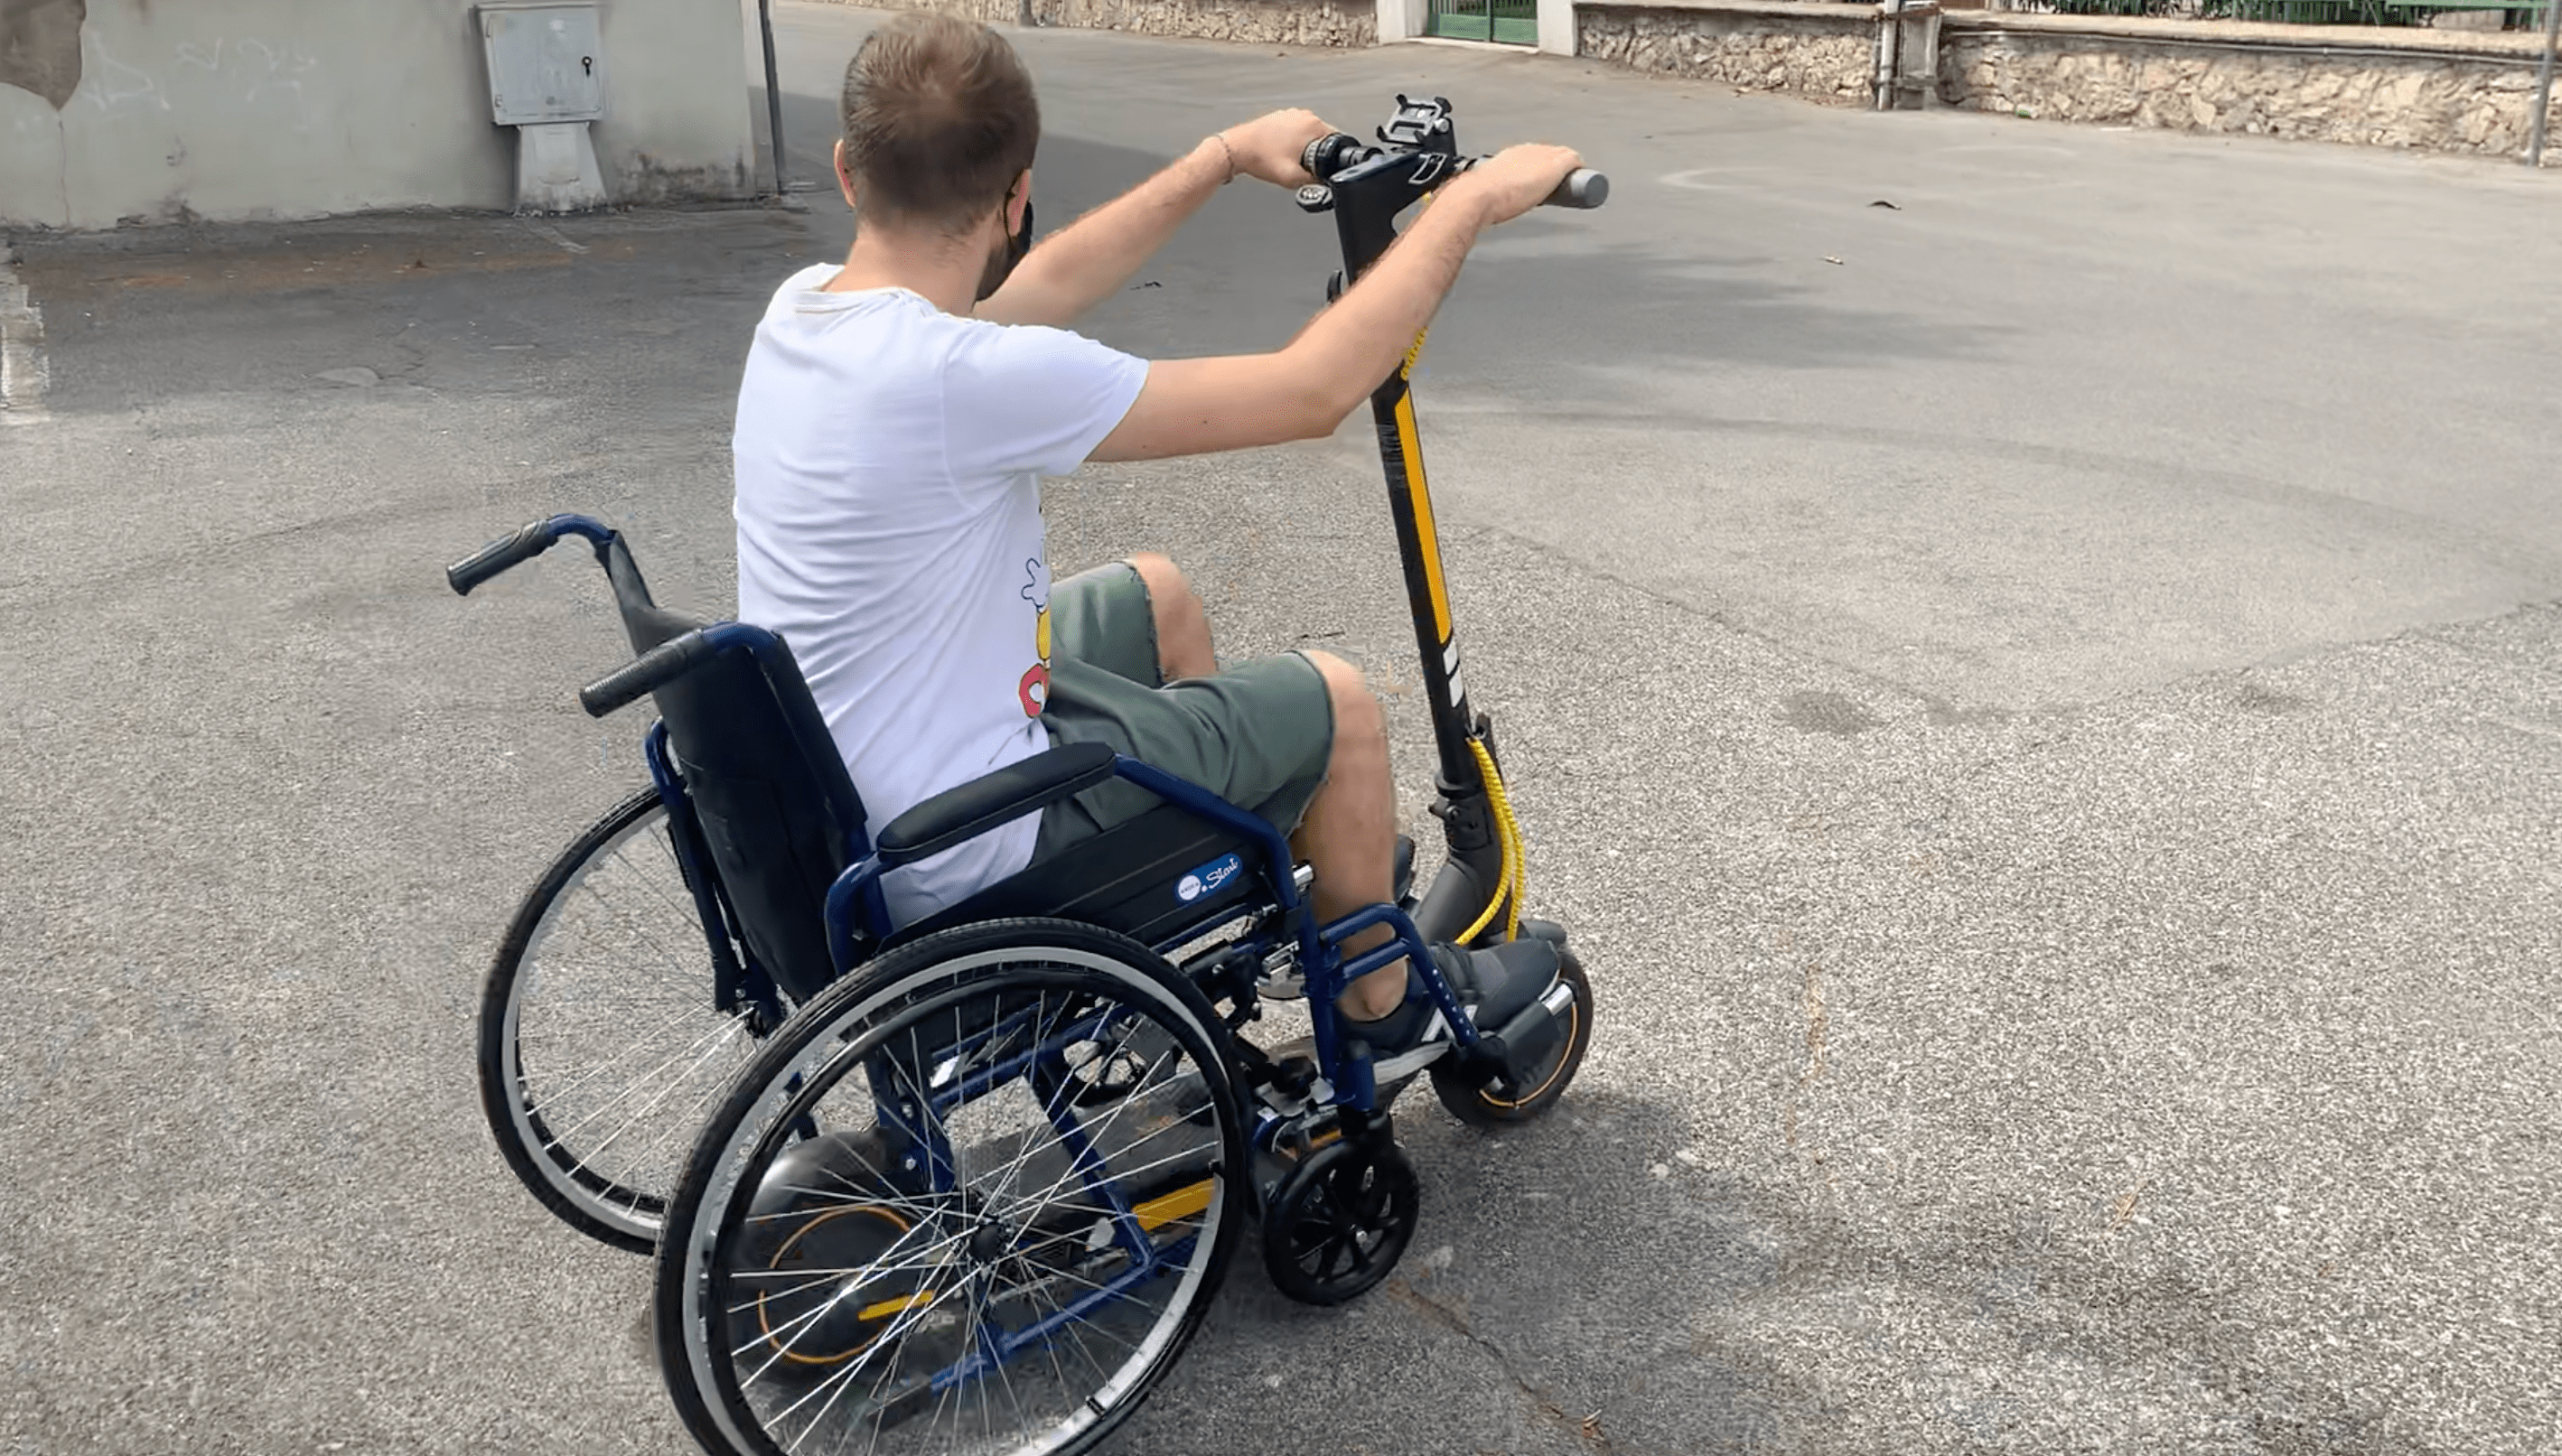
\includegraphics[width=.9\textwidth]{images/finished_project/IMG_2333.png}
    \caption{Second assembly method}
    \label{fig:second_ass_method2}
\end{figure}

\section{Experimental results}
Below we will illustrate numerous graphs aimed at showing the performance of the scooter with the standard firmware, driven without a wheelchair, and with the custom firmware created in this thesis, coupled to the wheelchair. Specifically, the graphs relating to current, battery discharge, temperature, residual distance, voltage and power supplied by the motor will be shown.

\begin{figure}[!htp]
\centering
    \begin{minipage}[t]{.45\textwidth}
    \centering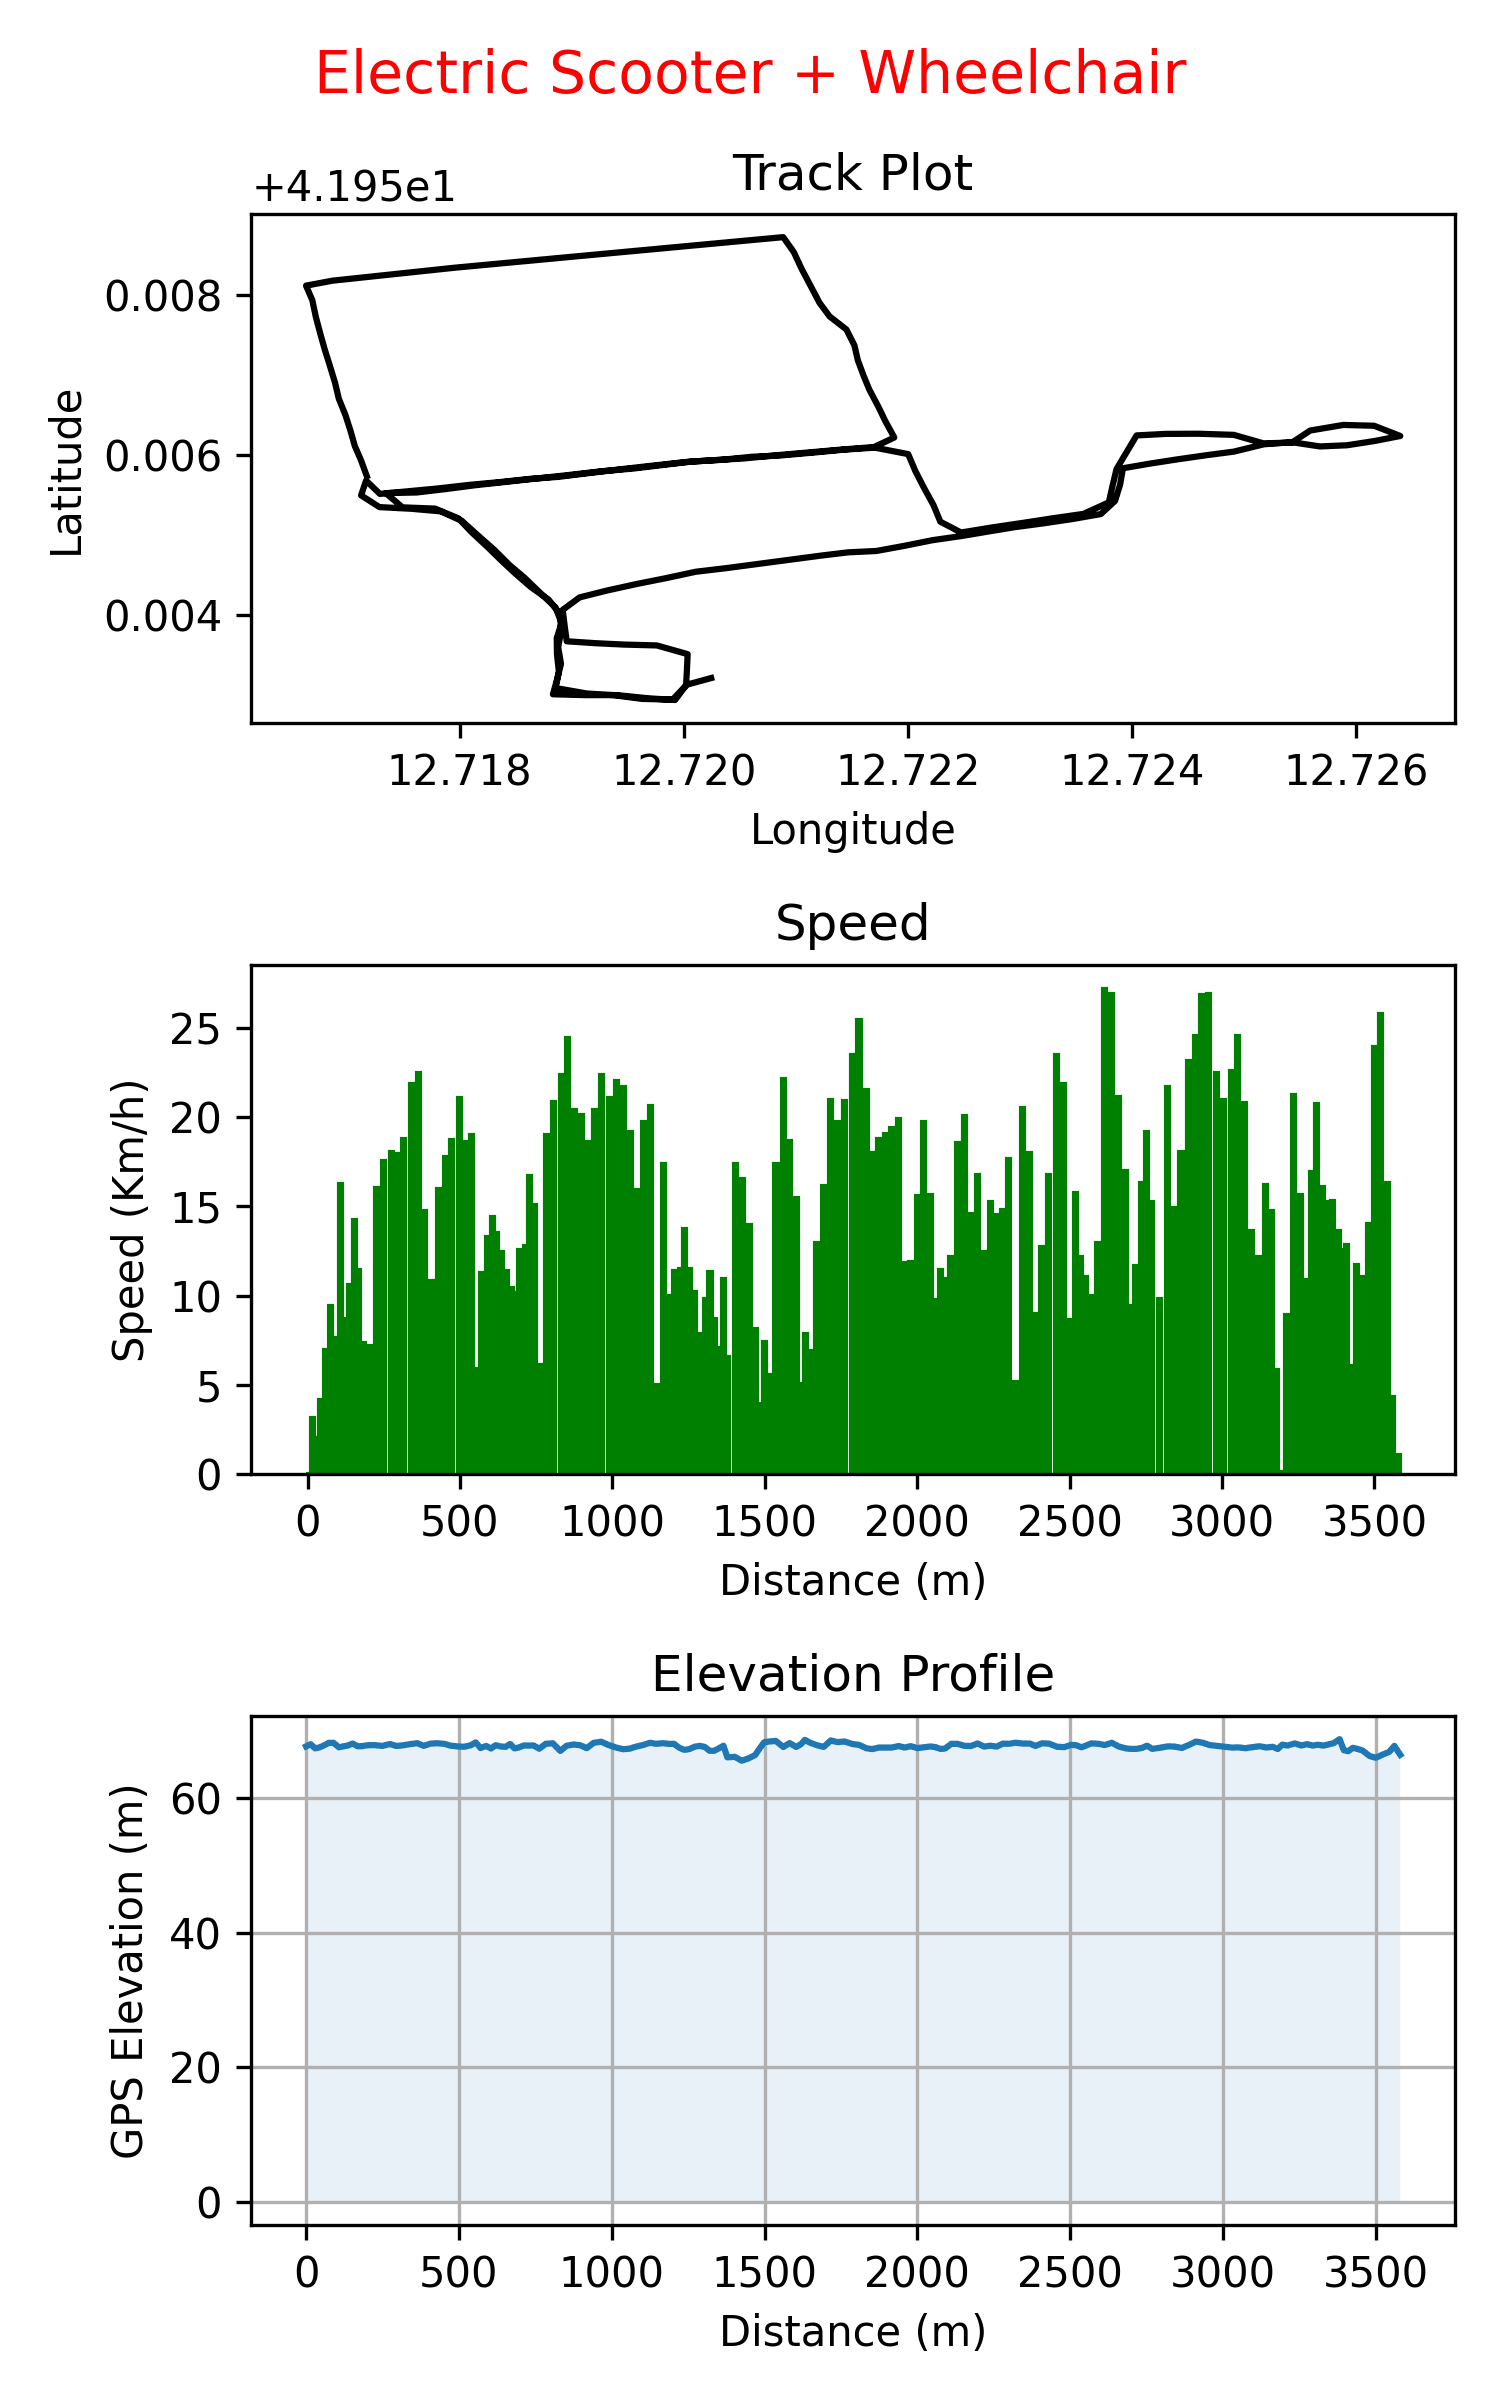
\includegraphics[width=.87\textwidth]{images/graphs/gpx1.png}
    \end{minipage}
    \begin{minipage}[t]{.45\textwidth}
    \centering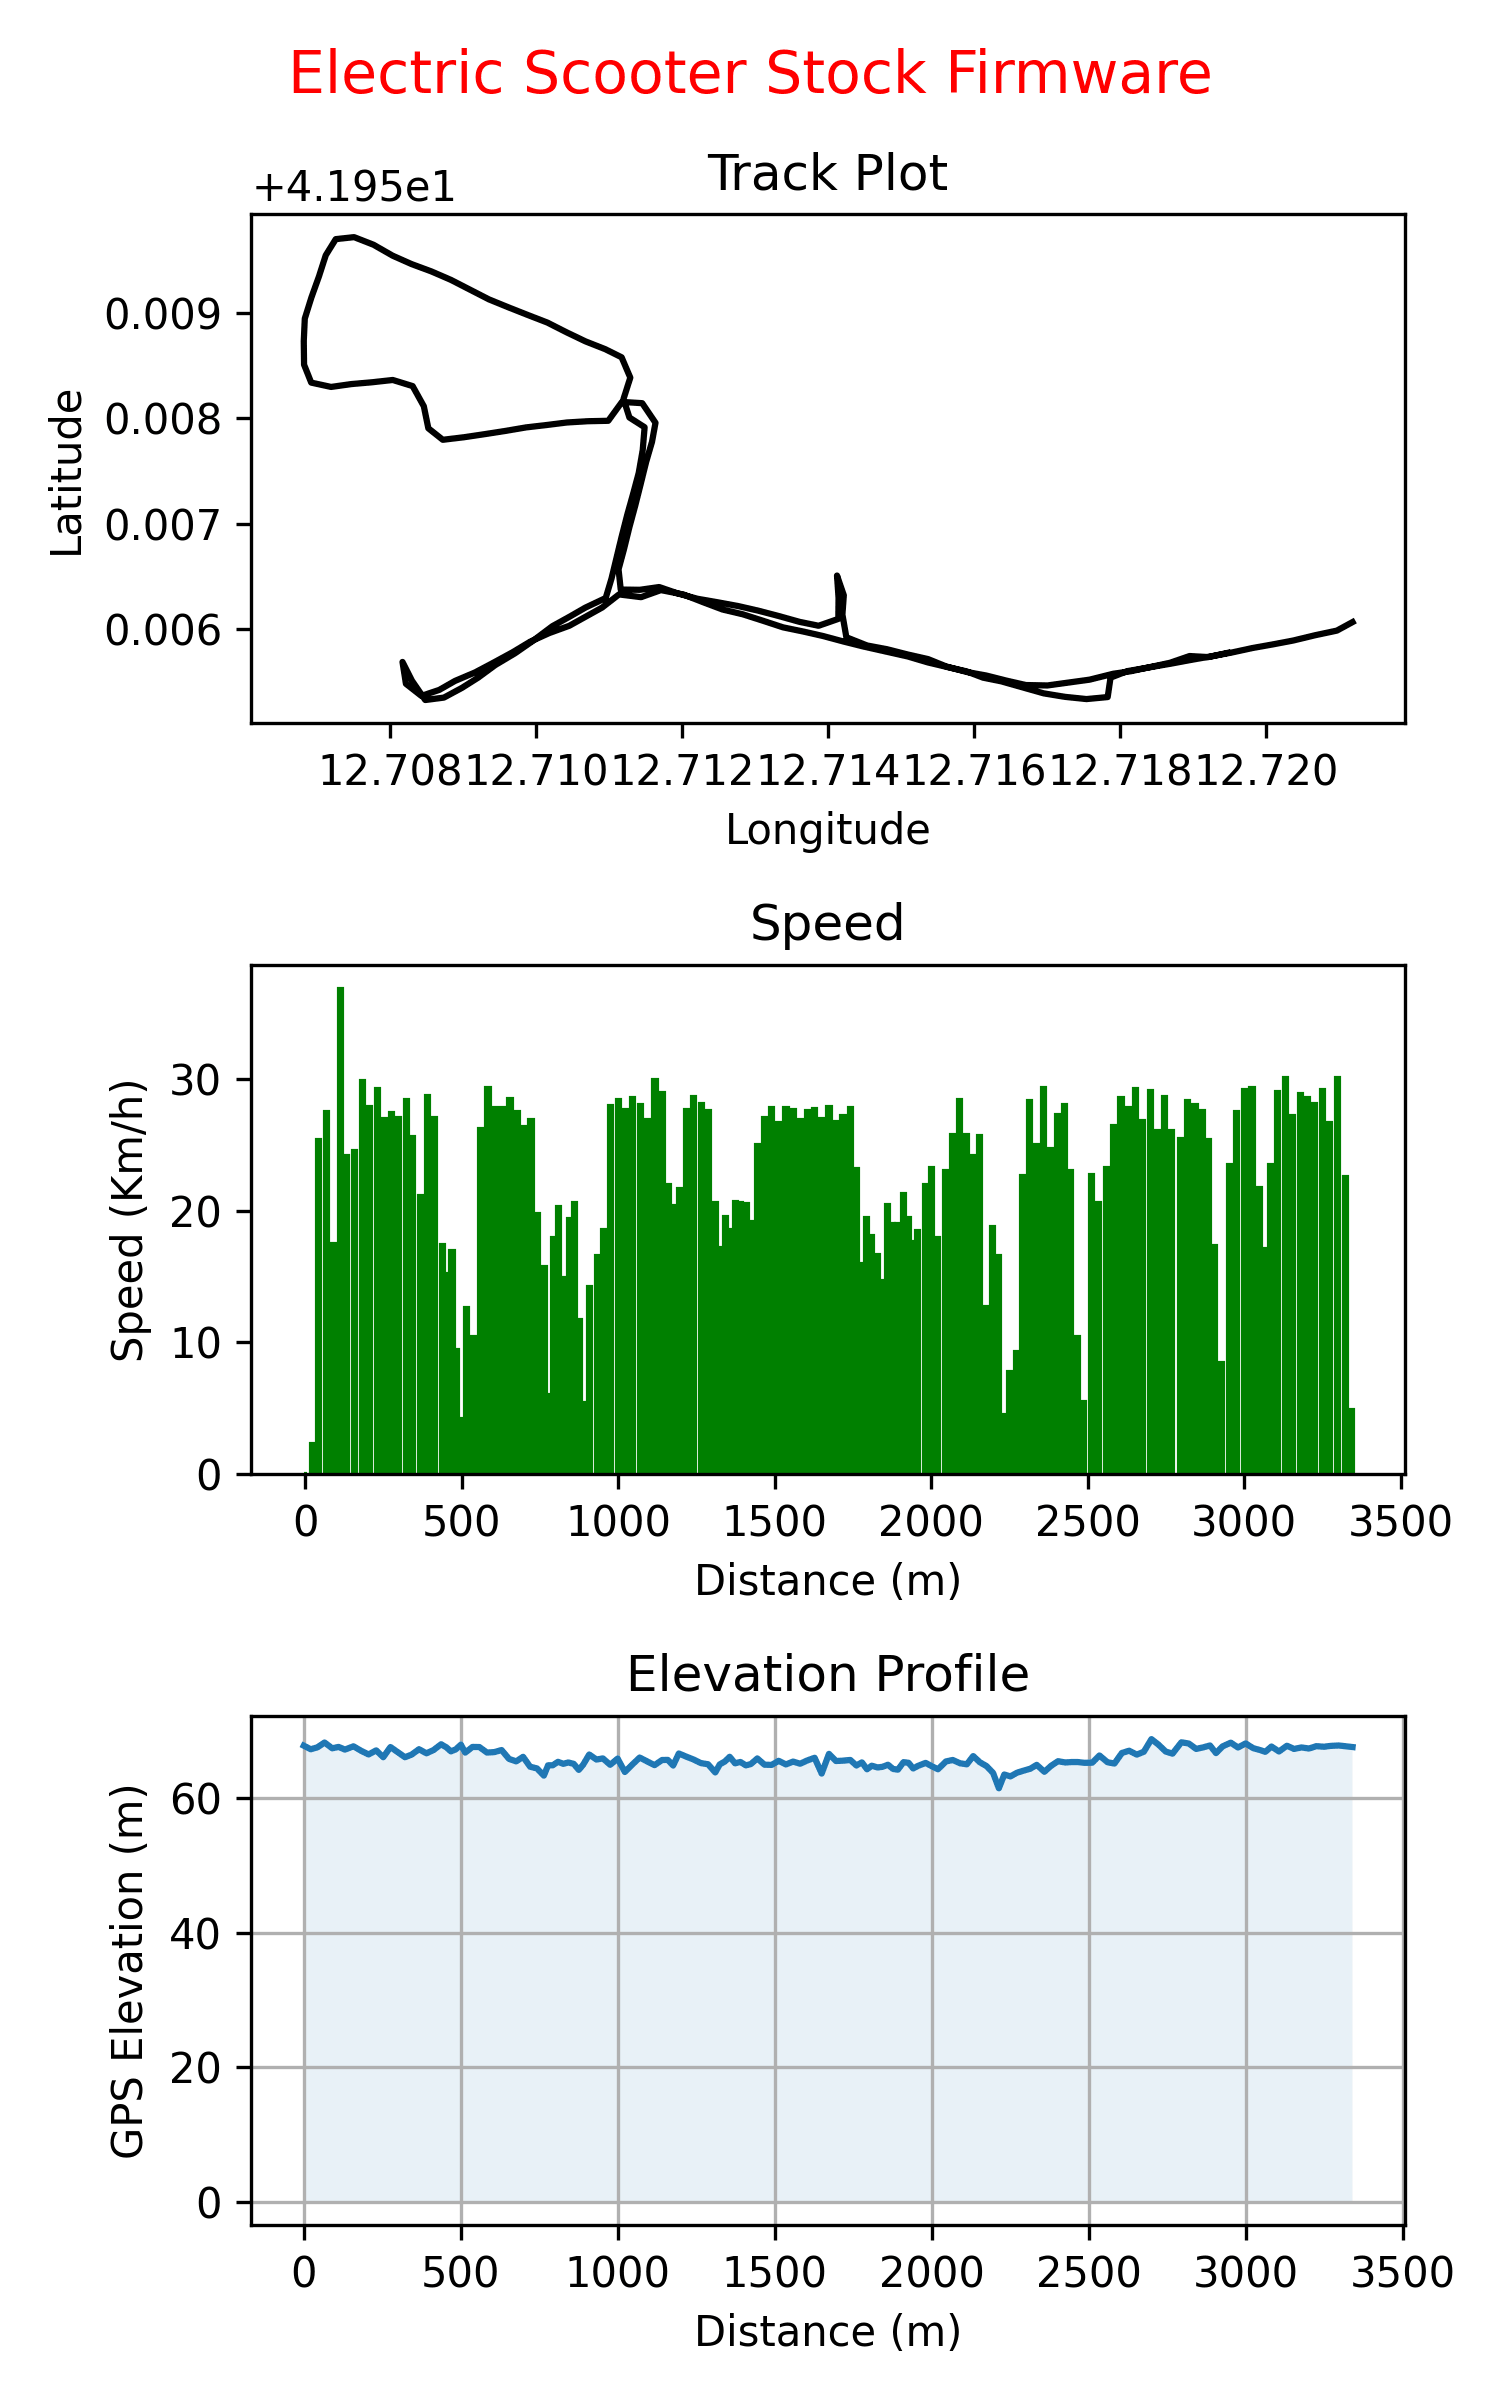
\includegraphics[width=.87\textwidth]{images/graphs/gpx2.png}
    \end{minipage}
    \caption{Distance traveled during the road test}
    \label{fig:distance_traveled}
\end{figure}

\newpage
\noindent As can be seen from the figure above, which shows 3 graphs relating to the position, speed and slope of the terrain, a road test lasting about 4 km was carried out on a mainly flat road at a speed as constant as possible.\\

\noindent From this point on we will show the graphs relating to the physical quantities that it was possible to acquire regarding the operation of the electric scooter.\\
In figure \ref{fig:1_curr&temp} it is possible to observe the trend of the current and the temperature over time and it can be seen that with respect to the first quantity there are positive peaks, relating to the acceleration phases and negative peaks relating to the braking phases in which the recovery system takes the windward. kinetic energy (KERS). It can be noted that the amplitude of these peaks is greater in the case of using the scooter with a wheelchair as the moving mass is greater and therefore during braking this system is able to recover a greater amount of energy. As for the temperature, it is possible to note that this reaches a range between 28 and 34 degrees centigrade, a range lower than that observed in the canonical use of the scooter and this is due to the way in which it was decided to map the law. acceleration, specifically with the use with a wheelchair the quadratic law was used with respect to the canonical linear law. This behavior therefore allows you to take advantage of a pleasant, functional and effective driving experience, while at the same time preserving the electronic components, primarily the battery, a component capable of exhibiting a highly variable behavior with respect to the temperature at which it operates. Therefore, operating at a lower temperature allows to extend the life of the battery and also to extend its duration, understood as the kilometers that can be traveled.

\begin{figure}[!htp]
    \centering
    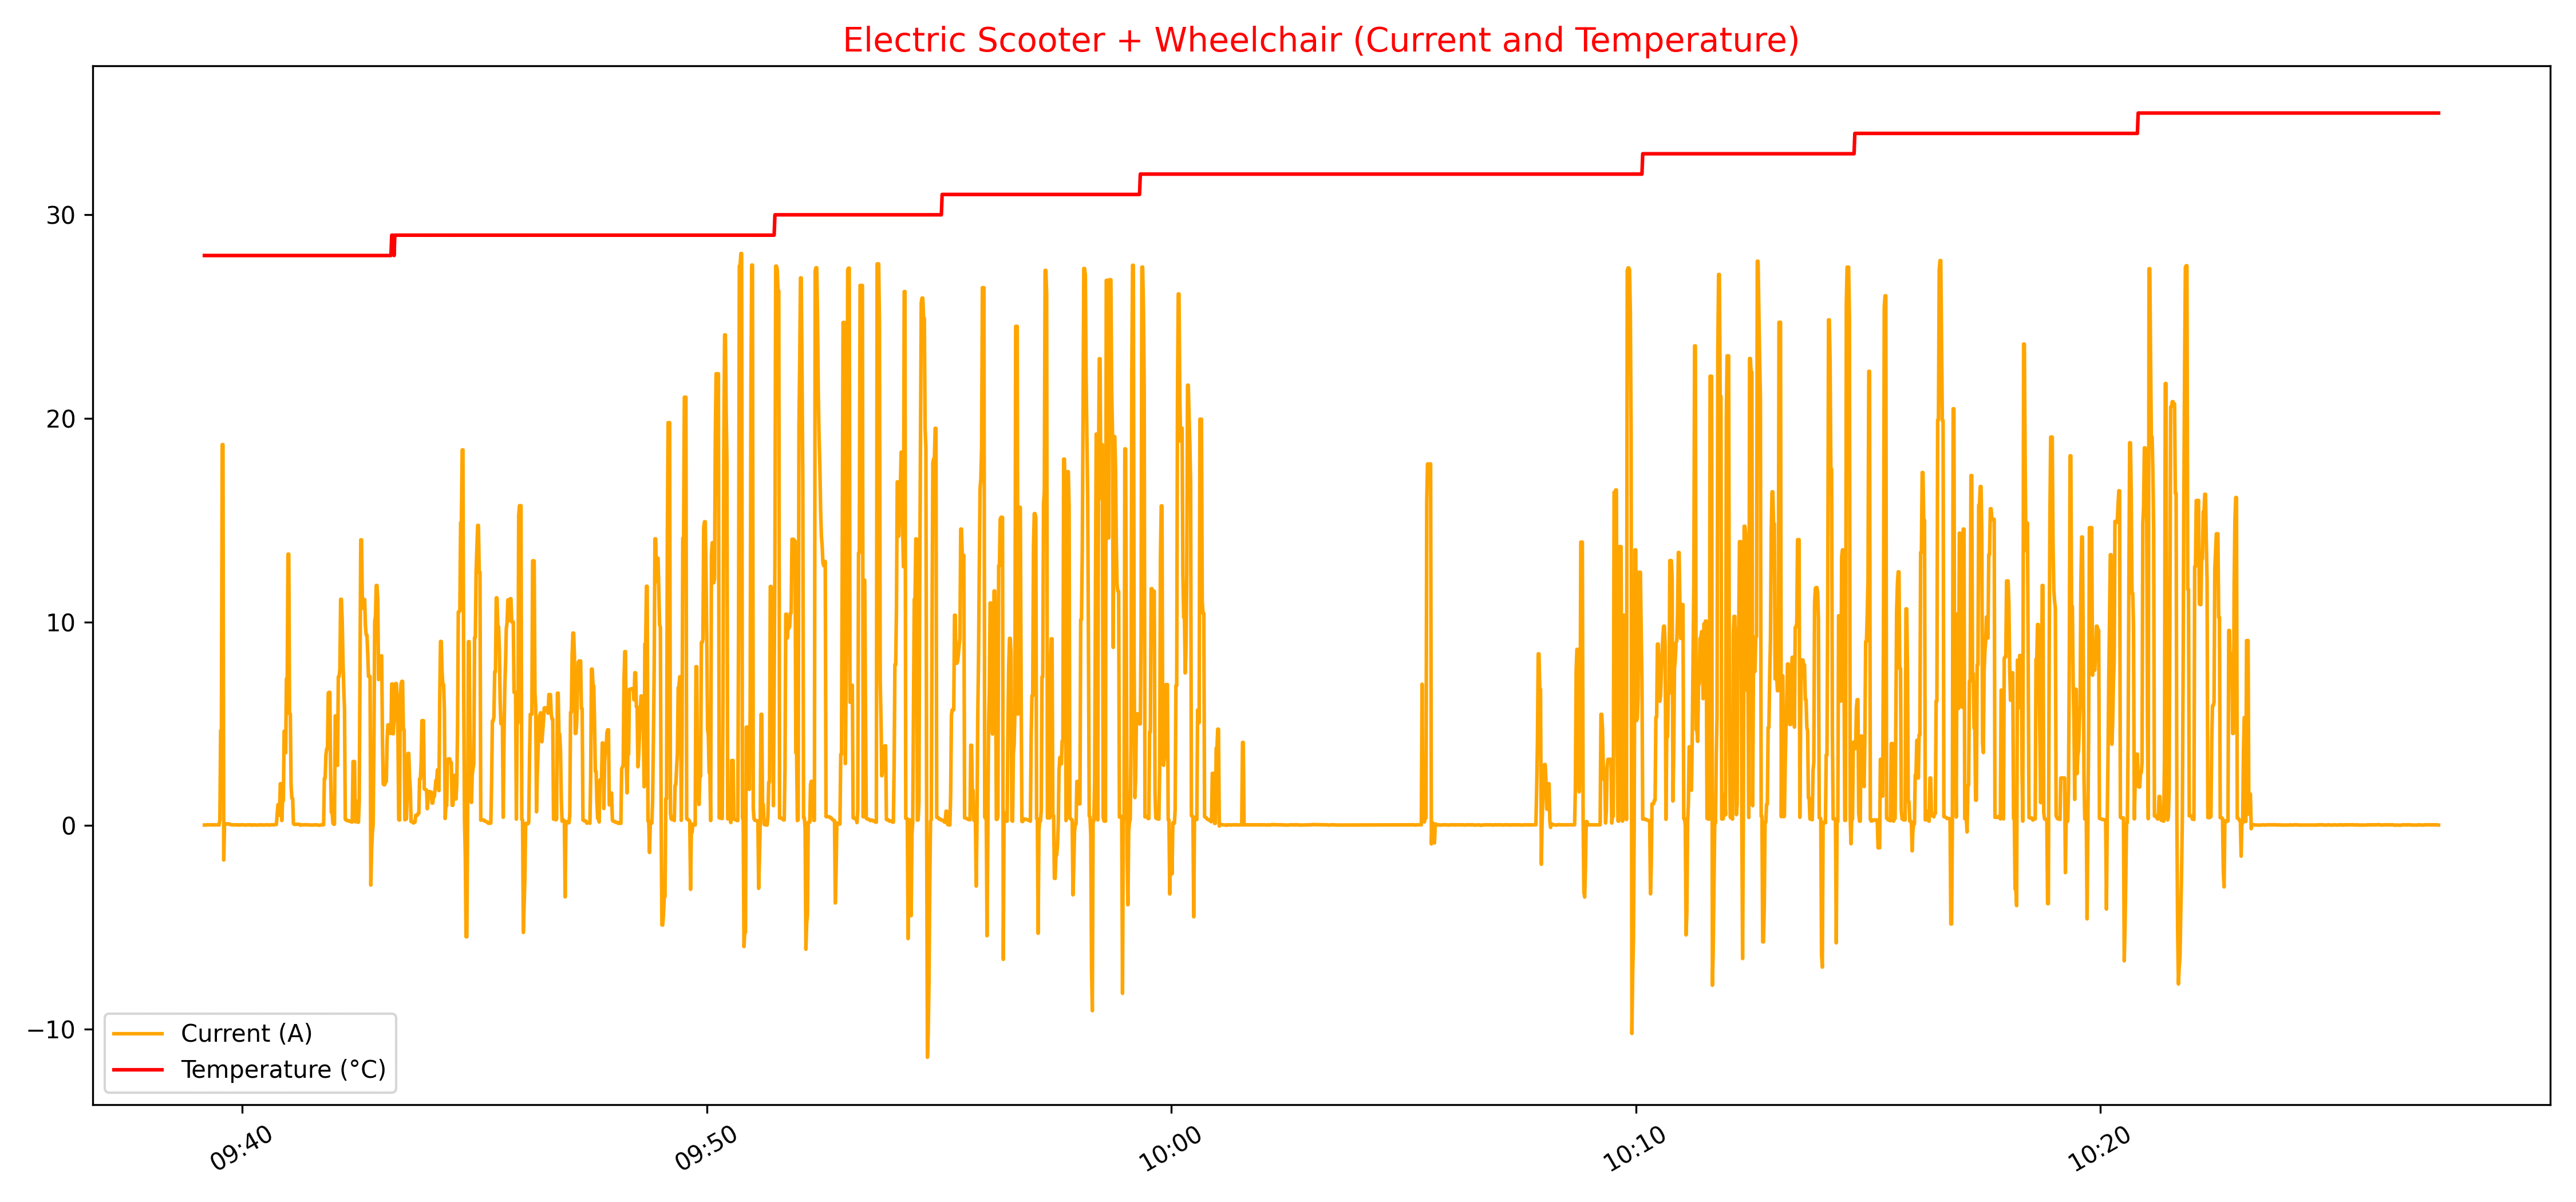
\includegraphics[width=.9\textwidth]{images/graphs/1_curr+temp.png}
    \caption{E-scooter + Wheelchair, current and temperature over time}
    \label{fig:1_curr&temp}
\end{figure}

\noindent Image \ref{fig:2_curr&temp} shows the trend over time of the current and operating temperature in the canonical use of the electric scooter equipped with stock firmware. it is possible to notice that there are many positive peaks as in the previous case but in this situation the negative peaks, therefore due to the recovery of kinetic energy, are of smaller amplitude due to the reduced mass. As far as the temperature is concerned, we can observe that this already in the initial phases is well above 35 degrees centigrade and how over time it reaches a temperature close to 40 degrees centigrade. As explained above, this significant difference is due to the different law that regulates acceleration and therefore the supply of current in the scooter. Specifically, the use of a linear law, the one present in the stock firmware, due to its nature provides for higher and extended current levels over time compared to the use of a quadratic or exponential law thus leading to higher operating temperatures.

\begin{figure}[!htp]
    \centering
    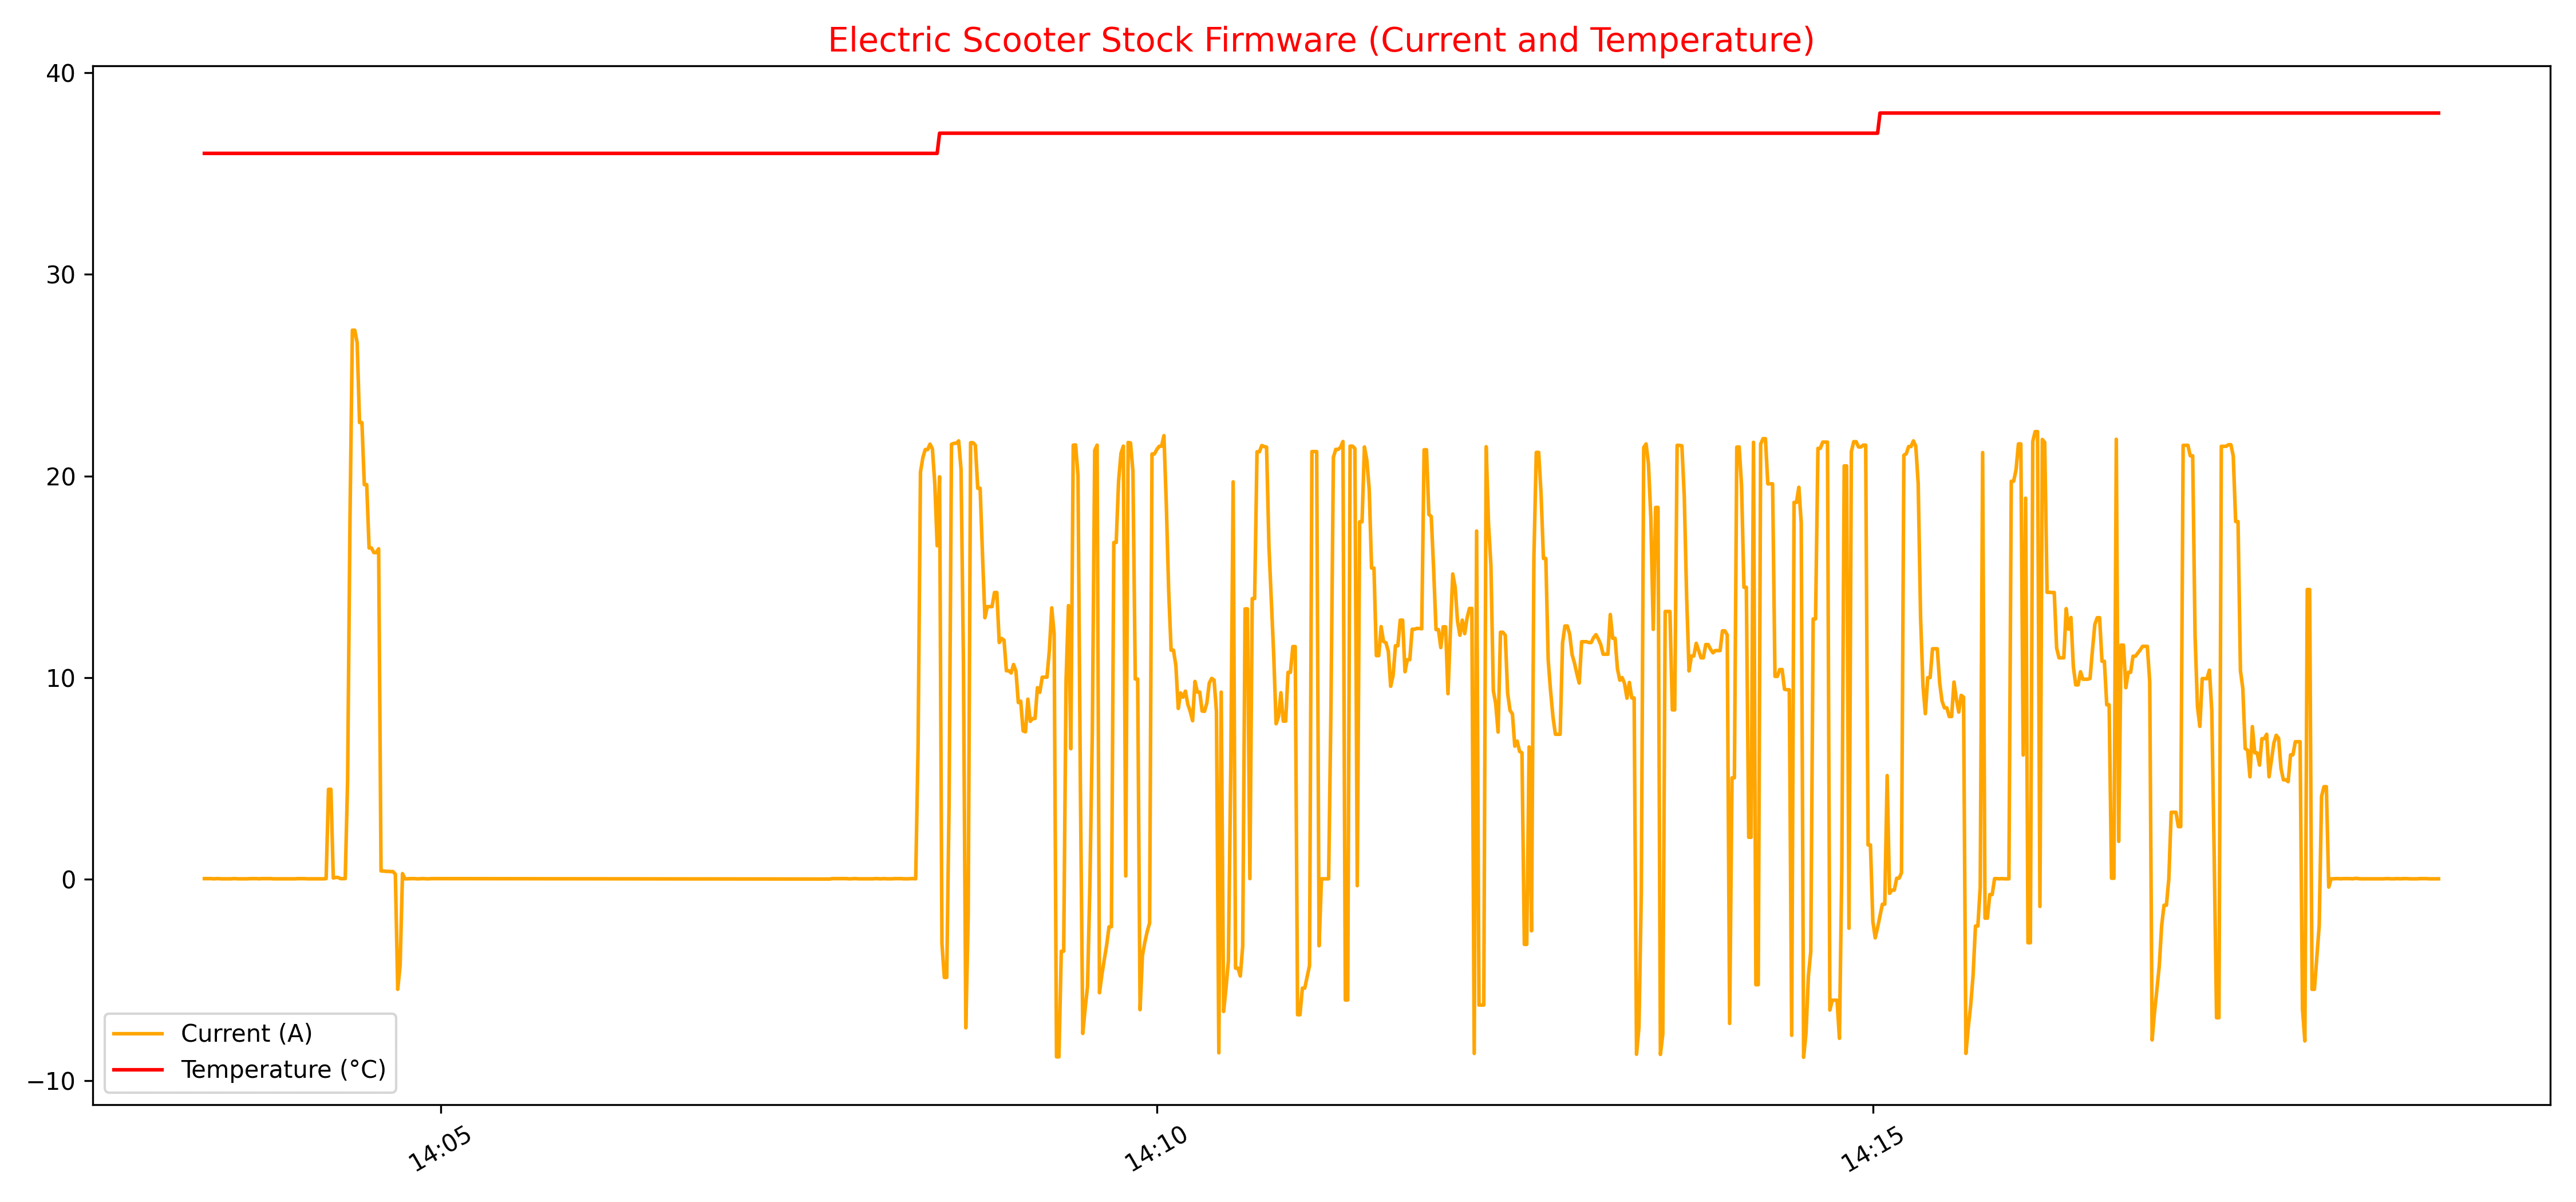
\includegraphics[width=.9\textwidth]{images/graphs/2_curr+temp.png}
    \caption{ E-scooter, Current and temperature over time}
    \label{fig:2_curr&temp}
\end{figure}

\noindent The following graphs will show the trend over time of the battery discharge, of the remaining distance and of the available voltage. Specifically in figure \ref{fig:1_batt&dist&volt} you can see these three trends in the case of using the electric scooter with custom firmware and coupled to a wheelchair and you can see how, due to the energy required by the motor to move a greater mass, the discharge of the battery it has a much steeper course than canonical use. In particular it can be noted that while in the canonical case the discharge presents a more regular trend over time, in the other case there are numerous charging and discharging phases or the steep discharges are compensated by the numerous times in which the KERS is able to recover the kinetic energy which in this case is greater. However, the energy requirement remains very high and the KERS can only slow down the relentless battery discharge which would have been much steeper without this energy recovery system.

\begin{figure}[!htp]
    \centering
    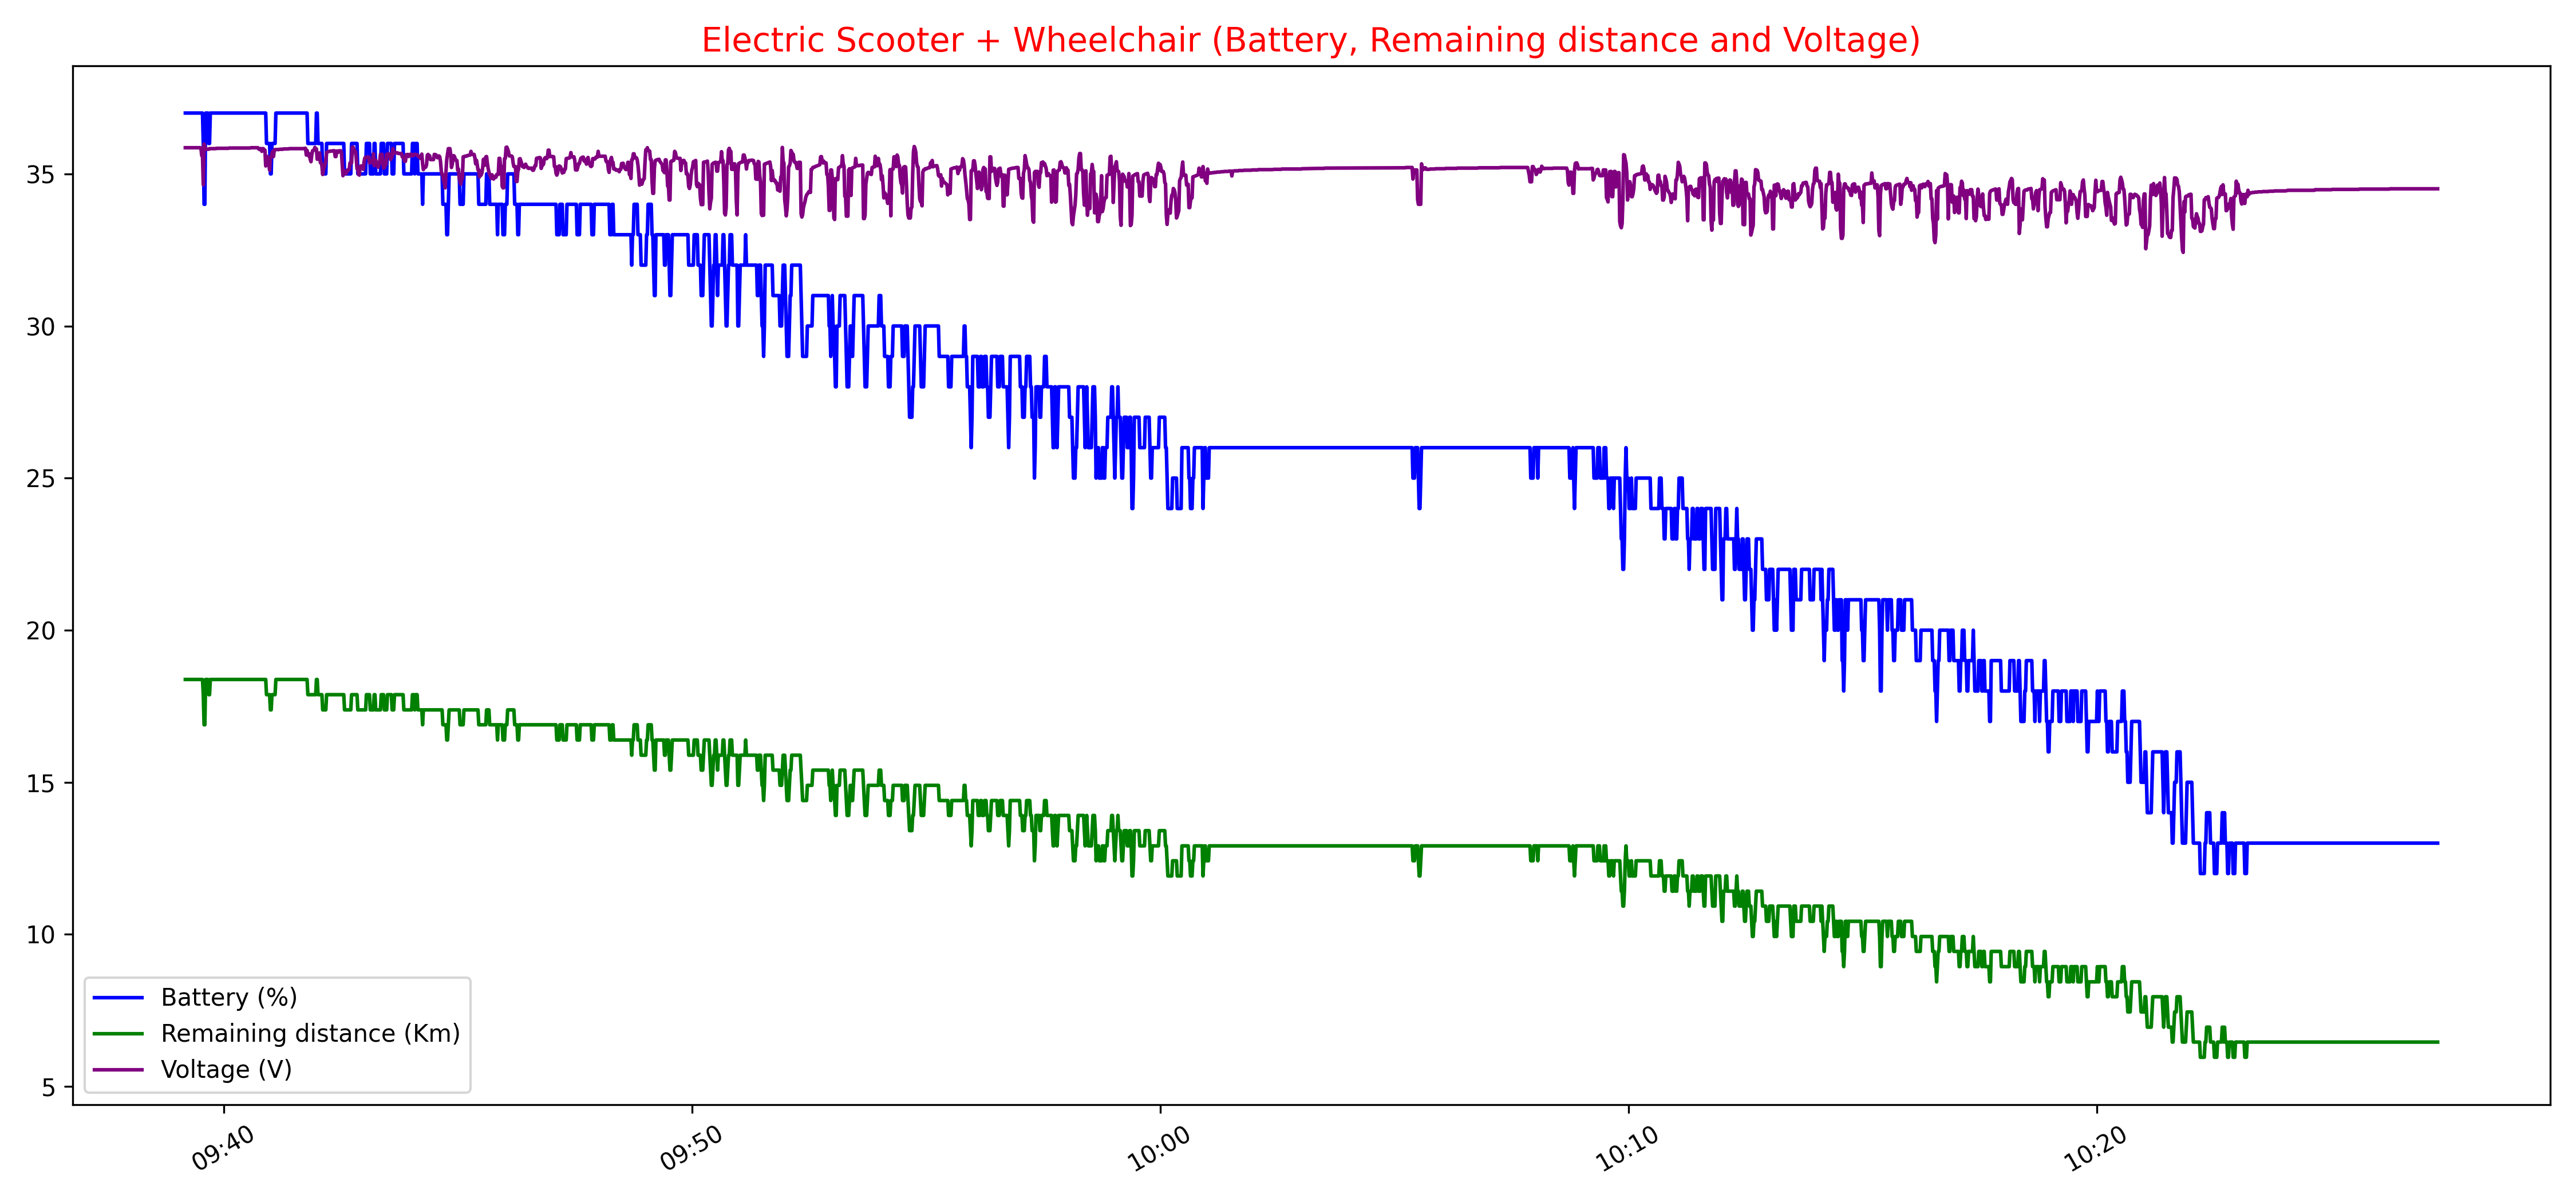
\includegraphics[width=.9\textwidth]{images/graphs/1_batt+dist+volt.png}
    \caption{E-scooter + Wheelchair,  Battery, remaining distance and voltage over time}
    \label{fig:1_batt&dist&volt}
\end{figure}

\newpage
\noindent In figure \ref{fig:2_batt&dist&volt} we can observe the trends shown previously for use with the standard firmware and how this is able to guarantee a more contained use of the available energy, both for the reduced mass to be towed, and for the different law that adjusts the acceleration. We can in fact note that the battery discharge phase is softer and with peaks relating to energy recovery of lower amplitude and frequency than in the previous case.

\begin{figure}[!htp]
    \centering
    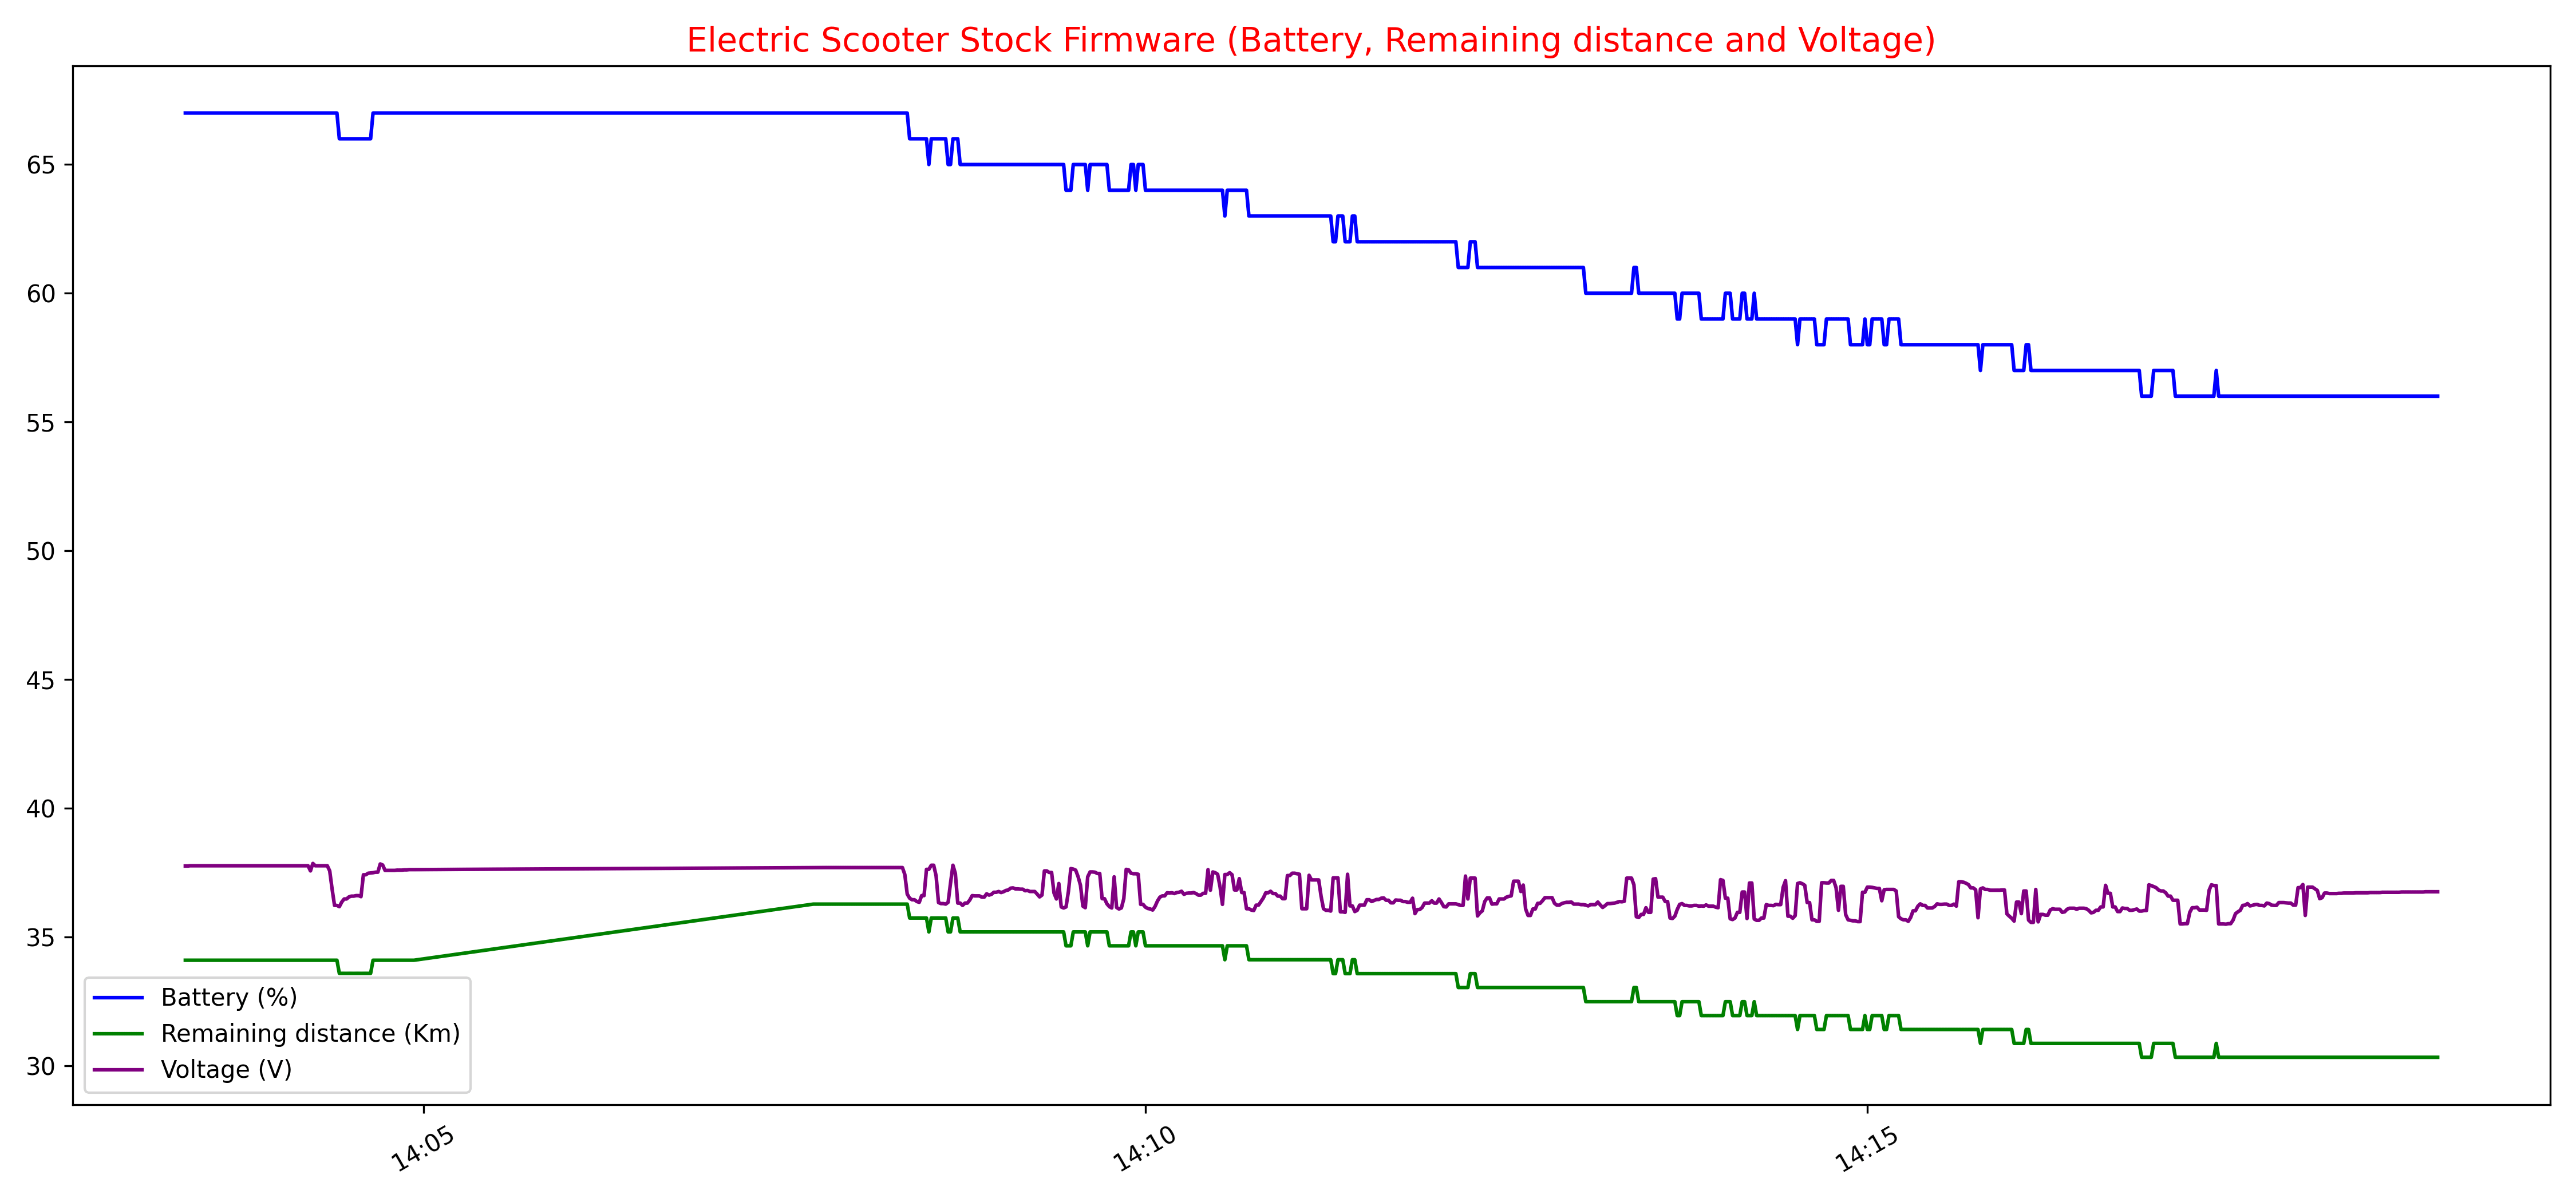
\includegraphics[width=\textwidth]{images/graphs/2_batt+dist+volt.png}
    \caption{E-scooter,  Battery, remaining distance and voltage over time}
    \label{fig:2_batt&dist&volt}
\end{figure}

\noindent The following figures show the power delivered by the engine during the typical use experiment and in particular it can be noted that in the case of using the scooter with custom firmware and wheelchair the power peaks are much higher than in the case with stock. firmware. This is necessary not only to allow the scooter to have a greater starting base than in the normal case but also to be able to carry out accelerations that allow the towing of a greater mass. 

\begin{figure}[!htp]
    \centering
    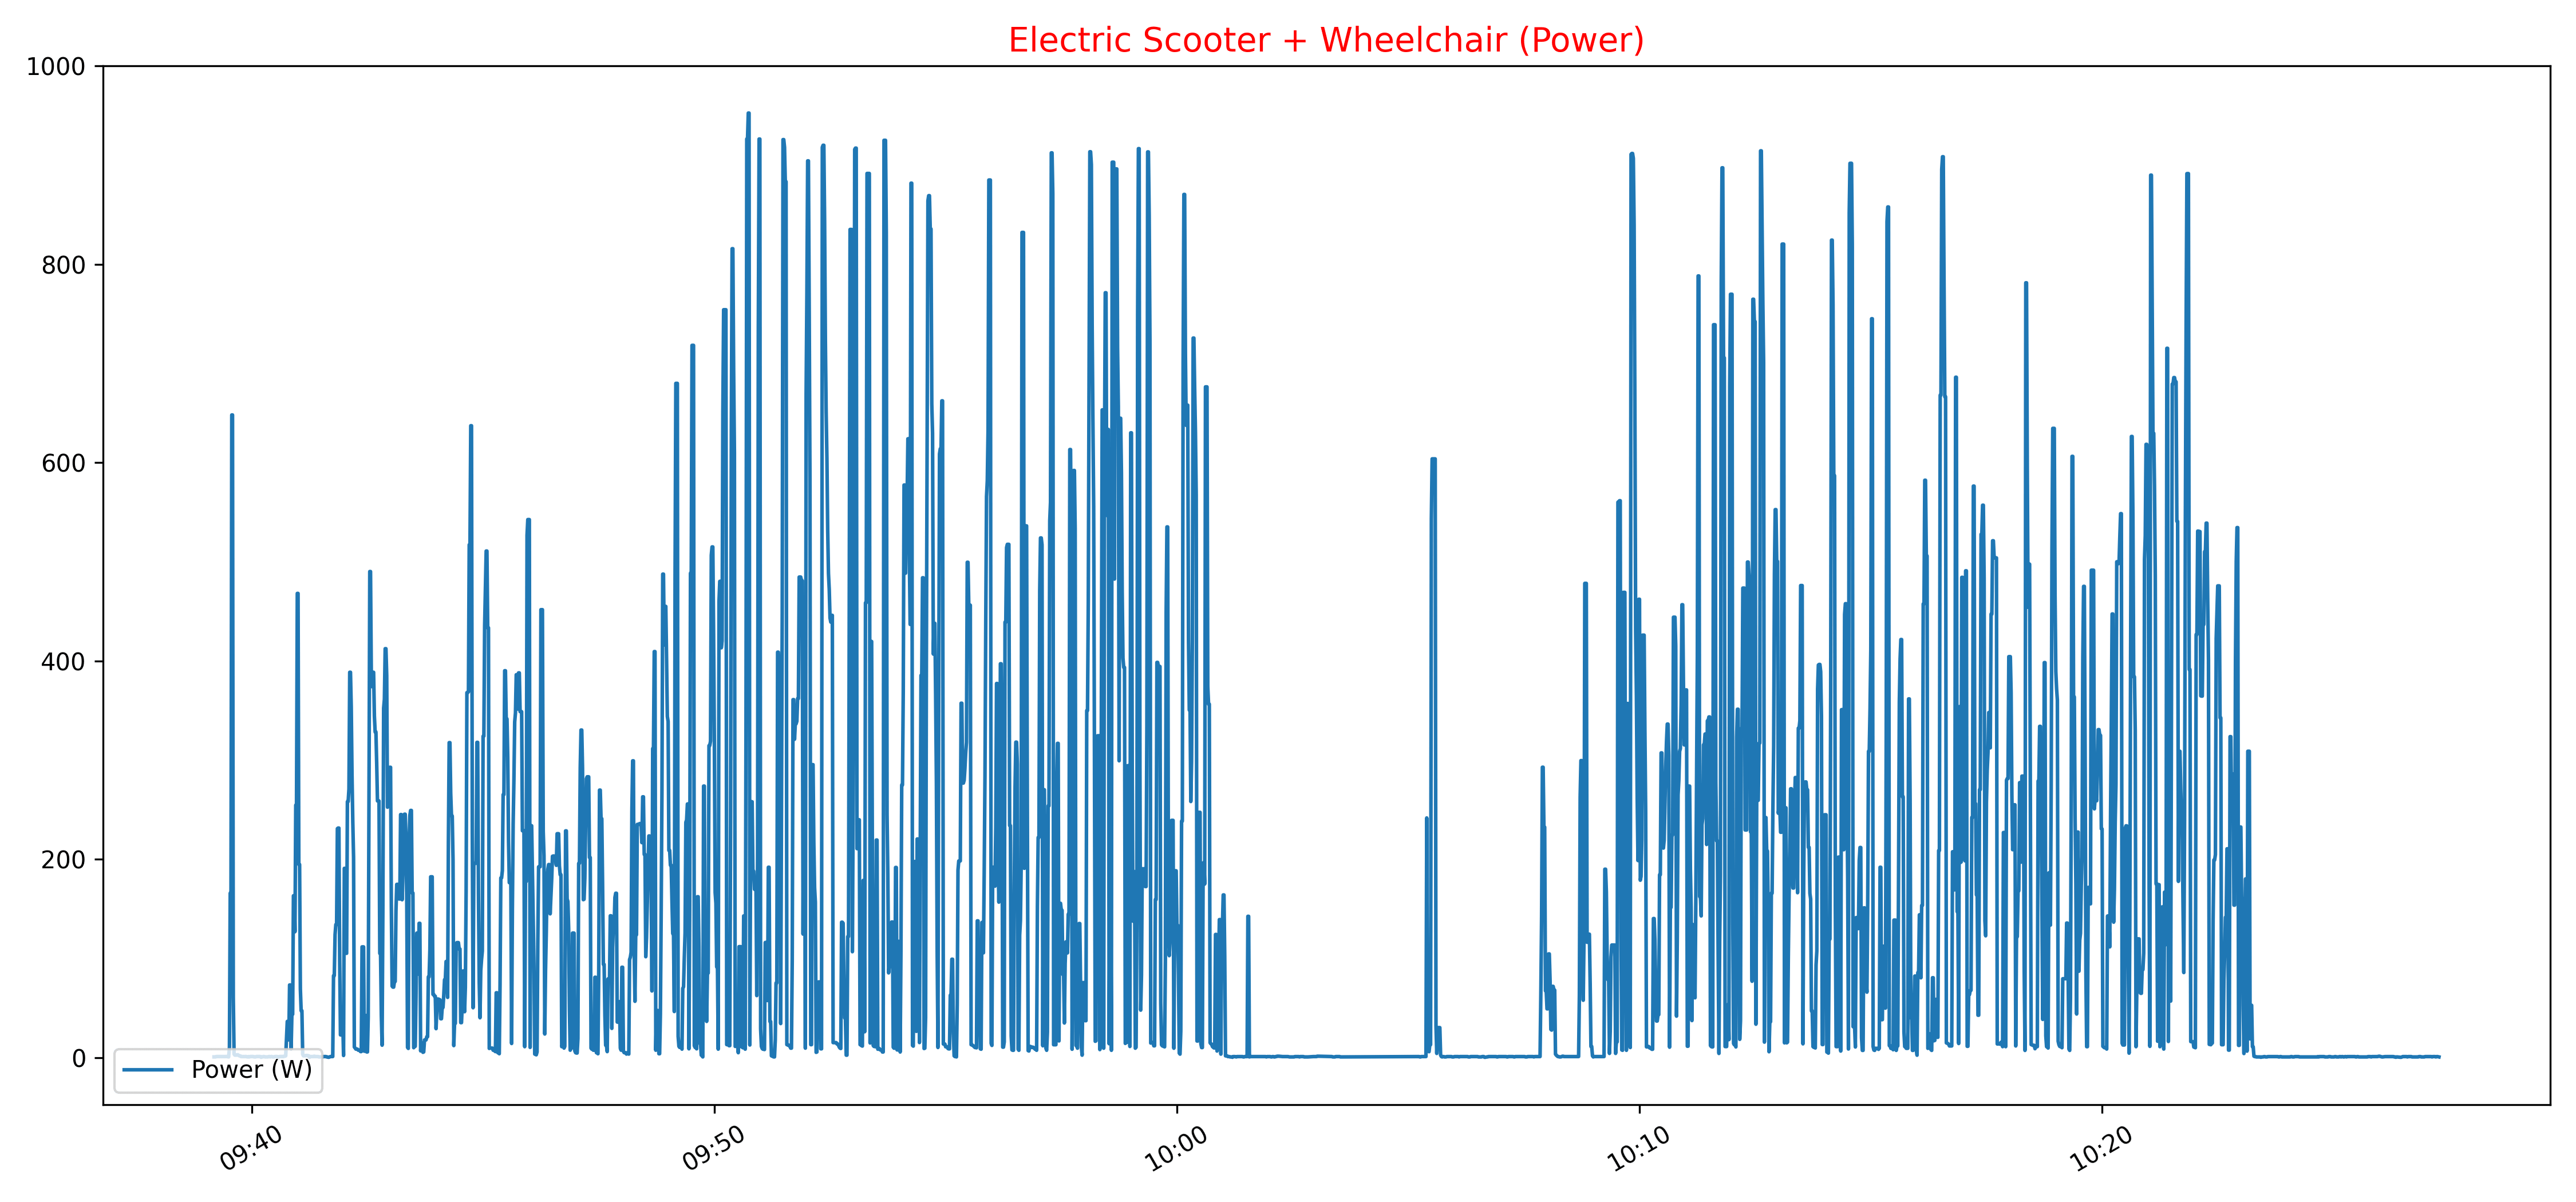
\includegraphics[width=\textwidth]{images/graphs/1_power.png}
    \caption{E-scooter + Wheelchair, Power over time}
    \label{fig:1_power}
\end{figure}

\newpage
\noindent It can be noted that in the case of stock firmware the average power level is 380W with peaks reaching 780W while in the case of custom firmware the average power delivered is about 550W with peaks of the order of 980W. These values are related only to one of the three driving modes of the electric scooter, sport mode since in the firmware customization phase it was decided to leave the other two modes unchanged to ensure longer battery life.

\begin{figure}[!htp]
    \centering
    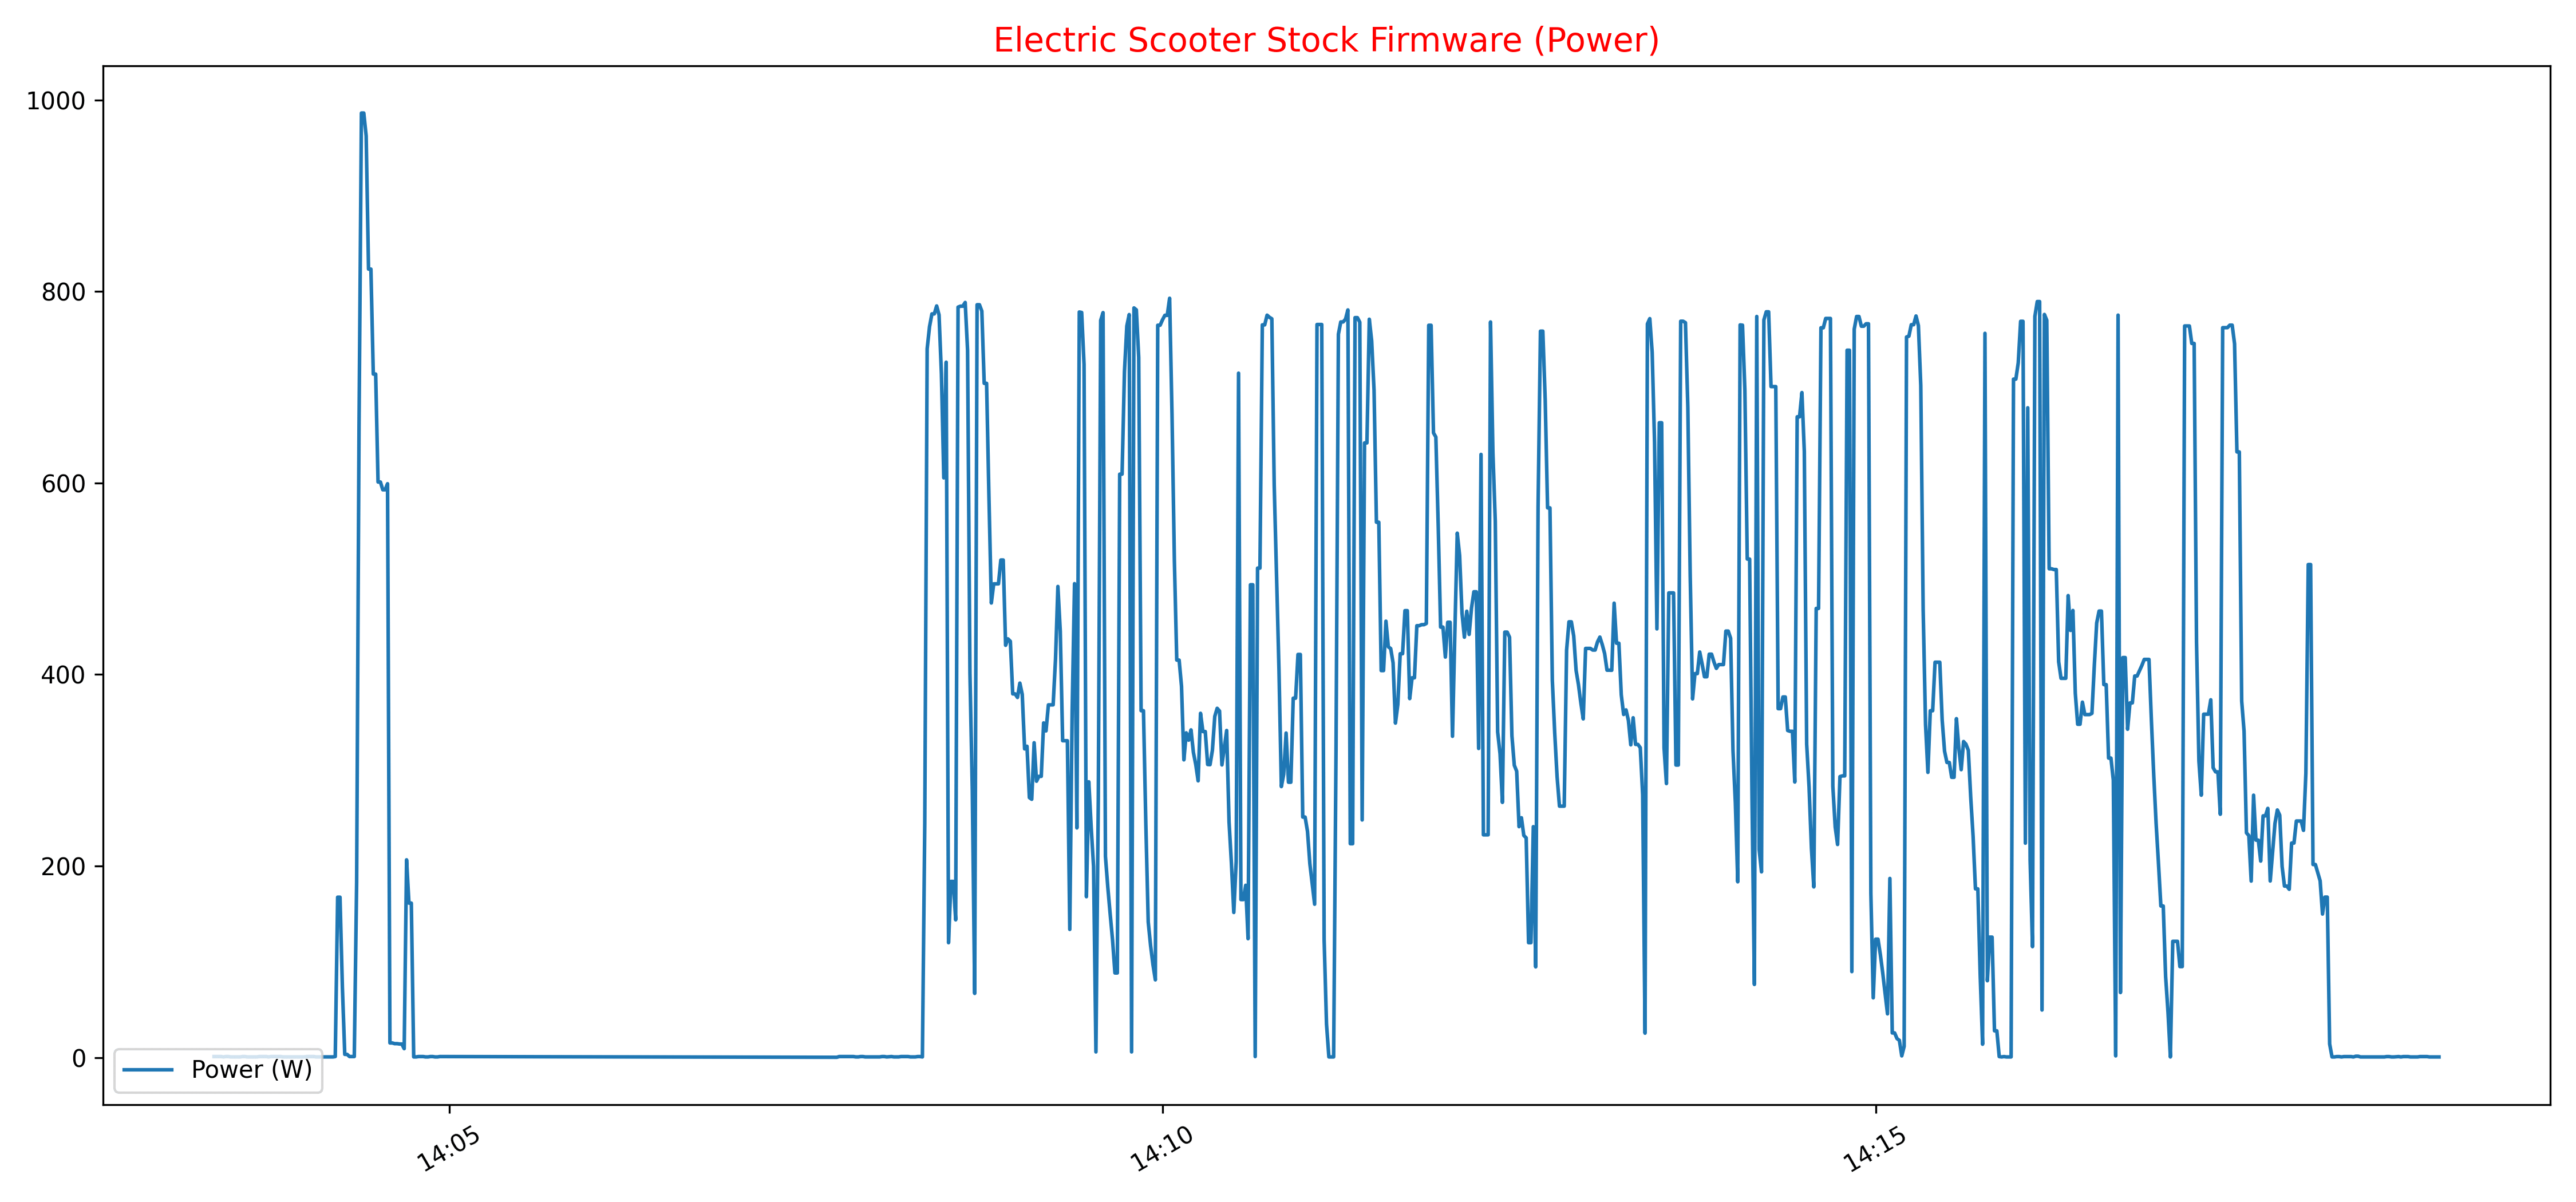
\includegraphics[width=\textwidth]{images/graphs/2_power.png}
    \caption{E-scooter, Power over time}
    \label{fig:2_power}
\end{figure}



\chapter{Conclusions and future works}
The aim of this thesis was to produce a first working prototype that allows any wheelchair owner to take advantage of the additional possibilities and functions offered by an electric scooter.\\
On the basis of the experiments, encouraging results emerged as it was possible to achieve the mechanical coupling between the two bodies and the modification of the firmware without affecting the functioning of the electric scooter and without adding further problems for the user. Furthermore, it was possible to achieve this without having to wrap the structure and nature of the scooter and the wheelchair, in such a way as to ensure their operation in a connection from the connection between the two.\\
On the other hand, less encouraging results also emerged from the experiments since, as shown in the chapter on assembly methods, both do not allow to have a 100\% efficient and effective guide since both modalities have advantages and limitations due to the physical structure of the two means of transport so heterogeneous. In particular, the main flaw relating to reduced visibility would be tackled when there are electric scooters with telescopic steering on the market which, however, are currently very little diffusion and in any case a modification of the steering would require a significant adaptation work. This problem would therefore not allow the use of shared electric scooters, unless they are equipped with a retractable or folding handlebar. On the other hand, the second mode would allow the electric scooter to be used by both able-bodied and disabled users, but at the expense of a reduced turning radius when using a wheelchair. We therefore believe that this second mode is the most suitable to be used on a permanent basis and that allows access to the benefits and potential of the electric scooter to the widest possible audience.\\
However, there is still a lot of work to be done as this project could be extended to a larger number of electric scooter and wheelchair brands. Companies operating in the electric scooter rental market could also be involved to share with them the results obtained in this thesis work thus allowing disabled people to be able to use the firmware modified according to their needs, with a simple request to the server via an application.\\
Further developments could be aimed at obtaining a finer tuning of the firmware parameters and therefore more effective and comfortable for driving by people with disabilities, also adapting it to the various engine models available on the market. Further room for improvement can be achieved by integrating state-of-the-art technologies into this project, for example through the use of machine learning for computer vision tasks. More specifically, video cameras could be integrated into the electric scooter and then used to be able to have a representation of the outside world and on the basis of this guarantee greater safety through the aid of machine learning algorithms, for example in helping the user to carry out the braking phase when an obstacle or a red light is detected.\\
In closing, further developments that have already been planned include the possibility of installing a seat belt on the wheelchair, an increased battery that allows the electric scooter's range to be extended, and a reinforcement of its control unit that allows for greater performance and faster motor reaction times. The reinforcement of the control unit consists in adding tin and possibly a copper wire in the rear tracks of the control unit itself, where high levels of current pass through. In this way there will be an increase in the diameter of the same which will allow not to have overheating. A broader and more advanced work can include the replacement of mosfets with higher quality components without causing any damage to the control unit with firmware that use higher currents.

\backmatter


\lstlistoflistings
\addcontentsline{toc}{chapter}{Listings}
\listoffigures
\addcontentsline{toc}{chapter}{\listfigurename}

\cleardoublepage
\phantomsection


% \end{thebibliography}
\backmatter
\nocite{*}
\printbibliography

\end{document}